\documentclass[journal]{new-aiaa}

\usepackage{lineno,hyperref}
\modulolinenumbers[5]
\usepackage{lineno,hyperref}
\usepackage{amssymb}
\usepackage{amsmath}
\usepackage{graphicx}
\usepackage{subfig}
%\usepackage{subcaption}
\usepackage{epstopdf}
\usepackage{subfiles}
%\usepackage{gensymb}
\usepackage{xcolor}
\usepackage{verbatim}
\usepackage{tikz}
\usepackage{pgfplots}
\usepackage{tikzscale}
\usepackage{mathabx}
\usepackage{epstopdf}
\usepackage[utf8]{inputenc}
\usepackage{booktabs}
\usepackage{dcolumn}

\usepackage[boxed]{algorithm2e}
\usepackage{mathrsfs}
\usepackage{breqn}
\usepackage{dsfont}
\usepackage[labelfont=bf]{caption}
\usepackage{amsmath,bm}
\usepackage{array,multirow}
\newcommand\myatop[2]{\left[{{#1}\atop#2}\right]} % "wrapper macro"

\title{Tailoring Snap-through Loads in Variable Stiffness Composites }

 \author{
     A.Haldar%
    \thanks{PhD Student, Institute of Structural Analysis, Appelstraße 9A, Hannover 30167, Germany}
  ,\ E.Jansen% 
  \thanks{Head of the group, Institute of Structural Analysis, Appelstraße 9A,  Hannover 30167, Germany}
  \ and R.Rolfes% 
  \thanks{Professor, Institute of Structural Analysis, Appelstraße 9A,  Hannover 30167, Germany}
  \\
  {\normalsize\itshape
   Leibniz Universität Hannover, 30167, Germany}\\
  \and
  P.M.Weaver%
   \thanks{§Professor in Lightweight Structures, Advanced Composite Centre for Innovation and Science, Queen’s Building, University Walk and Bernal Chair in Composite Materials and Structures, Bernal Institute,Limerick, Ireland and Member AIAA.}\\
  {\normalsize\itshape
  University of Bristol, Bristol, England BS8 1TR, United Kingdom}\\
 {\normalsize\itshape University of Limerick, Limerick, Ireland}
}


 % Data used by 'handcarry' option if invoked
 %  \AIAApapernumber{YEAR-NUMBER}
 %  \AIAAconference{Conference Name, Date, and Location}
 %  \AIAAcopyright{\AIAAcopyrightD{YEAR}}

 % Define commands to assure consistent treatment throughout document
 % \newcommand{\eqnref}[1]{(\ref{#1})}
 % \newcommand{\class}[1]{\texttt{#1}}
 % \newcommand{\package}[1]{\texttt{#1}}
  %\newcommand{\file}[1]{\texttt{#1}}
 % \newcommand{\BibTeX}{\textsc{Bib}\TeX}

\begin{document}

\maketitle

\begin{abstract}
Snap-through of multistable composites is a complex phenomenon that is difficult to characterize using simple analytical models. However, it is of paramount importance that the snap-through forces are accurately predicted if they are to be used in morphing structures. In this work, an accurate yet computationally fast model is proposed that computes the snap-through forces of variable stiffness (VS) laminates. The membrane problem is first solved exactly using differential quadrature method (DQM), and consequently, the in-plane stresses are written in terms of curvatures. The out-of-plane displacements are expressed in the form of Legendre functions, where the unknown coefficients of the displacement function are found using the Rayleigh-Ritz formulation. The calculated snap-through loads are then compared with Finite Element (FE) results.
\end{abstract}

\section{Introduction}

In the field of aerospace	 industry, shape changing capabilities offers significant improvement in the performance and can efficiently meet different operational requirements. In the recent past, multistable structures have shown a great potential in morphing applications \cite{Schultz2007,Mattioni2008application,Arrieta2014,Daynes2009,Diaconu2008}, especially due to the existence of multiple stable shapes and their ability to remain in these stable states without any external forces.

Multistable structures can be generated either by utilizing the differential thermal coefficient of an unsymmetric laminate in orthogonal directions \cite{Hyer1981}, or as a result of Gaussian curvature in initially curved shells \cite{seffen2007}, or due to prestressing \cite{Daynes2009}. 

However, thermally induced bistable shapes of unsymmetric laminates often result in a narrow range of shapes limiting its use in different applications. Recently, it was observed in Haldar et al. \cite{Haldar2017}
that variable stiffness (VS) laminates could be used to further tailor the stiffness properties of the plate, leading to a wider range of stable configurations than the constant stiffness laminates. For example, a cylindrical bistable configuration without any twisting curvature is typically constructed from $[0_n/90_n]$ unsymmetrical laminate. Similar shape can be also be generated using different options of VS configurations. Such composite laminates can be further tailored for the snap-through forces which an important parameter for efficient design of morphing structures.

In this paper, we exploit VS laminates to tailor the snap-through loads. We calculate the snap-through forces using a computationally efficient and robust technique build upon the method described in Lamacchia et al. \cite{Lamacchia2015}. It is previously seen in Diaconu et al. \cite{Diaconu2009}, that even for constant fiber laminates, the uniform curvature assumption fails to predict the snap-through loads, as it involves intermediate non-cylindrical shapes, which is also observed by Potter et al. 	\cite{Potter2007}experimentally.    

Higher order displacements are therefore necessary to capture the complex phenomenon of the snap-through event. However, with such approximations, the in-plane displacement or strain field results in expressions leading to high computational costs as observed in Mattioni et al. \cite{Mattioni2009} and Pirrera et al. \cite{Pirrera2010}. Nonlinear finite element (FE) proves to be an accurate tool, but high computational efforts may not be suitable for optimization or parametric studies. Therefore, a fast and sufficiently accurate analytical tool is required to study the snap-through behavior of VS laminates.

Lamacchia et al.\cite{Lamacchia2015} showed that Differential Quadrature Method (DQM) proves to be computationally efficient and robust tool to capture the snap-through behavior of straight fiber laminate. The key to this formulation is to decouple the bending and stretching parts from the total strain energy, using semi-inverse constitutive relation. As suggested by Vidoli et al.\cite{Vidoli2013}, it is crucial solving the membrane problem with negligible numerical error to evaluate the stretching energy accurately. In order to reduce the number of unknowns, the in-plane forces are expressed once and for all in terms of curvatures and thermal strains, using the compatibility equation and the constitutive relations. The total energy is then expressed as a function of just curvatures and thermal strains.

In this paper, the work of Lamacchia et al.\cite{Lamacchia2015} is extended for VS laminates.
% A linear variation of the fiber orientation angle proposed by Gürdal et al.\cite{Gurdal2008} is considered. 
The snap-through is triggered by applying four concentrated force at the corner of the plate. The contribution of the external forces is subsequently added to the total energy of the system.

All the possible equilibrium states are found by minimizing the total energy. The Hessian of the total potential energy with respect to the unknown coefficients of the displacement function indicates if the solution is stable or unstable. The developed model is subsequently compared with the FE results.

\section{Variable stiffness model}
\label{Path}
In this paper,  a curvilinear fiber path definition for the composite laminate is employed.  Although there can be different ways to vary the fiber path in a curvilinear pattern, the linear variation of the fiber orientation angle proposed by G{\"u}rdal et al. \cite{Gurdal2008} is considered in this work. Such linear variation is more practical due to its adaptability to  manufacturing constraints, and also useful in building simpler analytical models.

\begin{figure}[!htb]
	\centering
	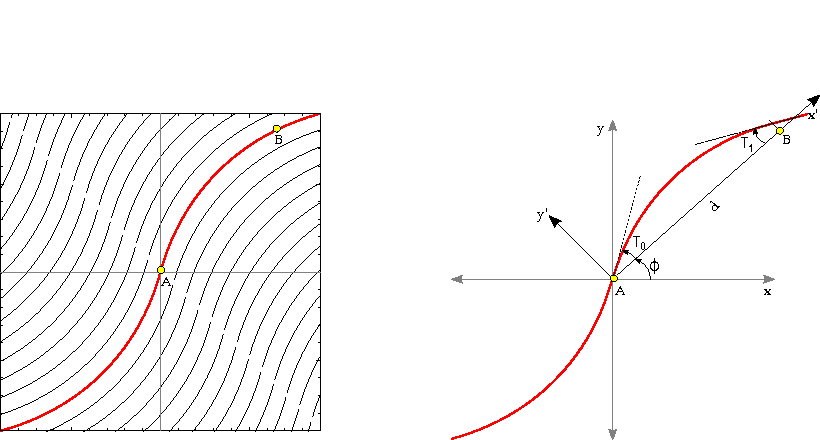
\includegraphics[ width=.75\textwidth ]{figures2/fiberdef.pdf}
	\caption{Parameters defining the curvilinear fiber path}
	\label{fig:fiberdef}
\end{figure}

The fiber orientation angle $\theta$  is defined as follows:

\begin{equation}
\label{fibdef2}
\begin{aligned}
\theta(x')=
\phi+\frac{\left(T_1-T_0\right)|x'|}{d} + T_0
\end{aligned}
\end{equation}
where
\begin{equation}
\label{fibdef3}
\begin{aligned}
x'&= x\cos{\phi}+y\sin{\phi}
% d &= \left(X_1-X_0\right)\cos{\phi}+ %\left(Y_1-Y_0\right)\sin{\phi}
\end{aligned}
\end{equation}


\section{Model}
\subsection{Kinematics}
A material point in the deformed configuration can be expressed as $\textbf{x} = \textbf{X} + \textbf{u}$, where $\textbf{u} (u, v, w)$ denotes the displacement vector in the $x$, $y$ and $z$ direction, whereas $\textbf{x}$, $\textbf{X}$ identify the position vectors in the undeformed and in the reference configuration, respectively. The components of the displacement vector are defined accordingly as:
\begin{equation}
\label{disp}
u(x,y,z)  = u_{0}(x,y)  -  z \frac{\partial w_{0}}{\partial x},  \hspace {0.2cm}
v(x,y,z)  = v_{0}(x,y)  -  z \frac{\partial w_{0}}{\partial y} ,  \hspace {0.2cm}
w(x,y,z)  = w_{0}(x,y)
\end{equation}
where the subscript $0$ identifies the mid-plane displacements. 

The strain components includes non-linear von K\'arm\'an strains under the assumption of small strains and moderate rotations are given by:
%\begin{equation}
%\label{strain}
%\varepsilon_{xx}   = \frac{\partial u}{\partial x}  +  \frac{1}{2}  \left(\frac{\partial w}{\partial x} \right)^2,  \hspace {0.2cm} \varepsilon_{yy}  = \frac{\partial v}{\partial y}  +  \frac{1}{2}  \left(\frac{\partial w}{\partial y} \right)^2,  \hspace {0.2cm}
%\gamma_{xy} = \frac{\partial u}{\partial y} + \frac{\partial v}{\partial x} + \frac{\partial w}{\partial x}\frac{\partial w}{\partial y}
%\end{equation}
%which shows the non-linear strain displacement relationships. By inserting Eq. \eqref{disp} into Eq. \eqref{strain}, the strain relations can be rearranged as:
%\begin{equation}
%\label{strain1}
%\boldsymbol \varepsilon =  \begin{bmatrix}
%\varepsilon_{xx} \\ \varepsilon_{yy} \\ \gamma_{xy}
%\end{bmatrix} =
%\begin{bmatrix}
%\epsilon_{xx} \\ \epsilon_{yy} \\ \epsilon_{xy}
%\end{bmatrix} + z
%\begin{bmatrix}
%\kappa_{xx} \\ \kappa_{yy} \\ \kappa_{xy}
%\end{bmatrix}  =
%\begin{bmatrix}
%\frac{\partial u_{0}}{\partial x}  +  \frac{1}{2}  \left(\frac{\partial w_{0}}{\partial x} \right)^2 \\
%\frac{\partial v_{0}}{\partial y}  +  \frac{1}{2}  \left(\frac{\partial w_{0}}{\partial y} \right)^2 \\
%\frac{\partial u_{0}}{\partial y}  + \frac{\partial v_{0}}{\partial x} +\frac{\partial w_{0}}{\partial x}\frac{\partial w_{0}}{\partial y}
%\end{bmatrix} +
%z   \begin{bmatrix}
%- \frac{\partial^{2} w_{0}}{\partial x^{2}} \\
%- \frac{\partial^{2} w_{0}}{\partial y^{2}}  \\
%-2 \frac{\partial^{2} w_{0}}{\partial x \partial y}
%\end{bmatrix} =
%\epsilon + z  \kappa,
%\end{equation}
%where $\epsilon$ and $\kappa$ represent the mid-plane strain and curvature vectors, respectively.


\begin{equation}
\label{strain}
\epsilon_{xx}   = \frac{\partial u}{\partial x}  +  \frac{1}{2}  \left(\frac{\partial w}{\partial x} \right)^2,  \hspace {0.2cm} \epsilon_{yy}  = \frac{\partial v}{\partial y}  +  \frac{1}{2}  \left(\frac{\partial w}{\partial y} \right)^2,  \hspace {0.2cm}
\gamma_{xy} = \frac{\partial u}{\partial y} + \frac{\partial v}{\partial x} + \frac{\partial w}{\partial x}\frac{\partial w}{\partial y}
\end{equation}
which shows the non-linear strain displacement relationships. By inserting Eq. \eqref{disp} into Eq. \eqref{strain}, the strain relations can be rearranged as:
\begin{equation}
\label{strain1}
\boldsymbol \epsilon =  \begin{bmatrix}
\epsilon_{xx} \\ \epsilon_{yy} \\ \gamma_{xy}
\end{bmatrix} =
\begin{bmatrix}
\varepsilon_{xx} \\ \varepsilon_{yy} \\ \varepsilon_{xy}
\end{bmatrix} + z
\begin{bmatrix}
\kappa_{xx} \\ \kappa_{yy} \\ \kappa_{xy}
\end{bmatrix}  =
\begin{bmatrix}
\frac{\partial u_{0}}{\partial x}  +  \frac{1}{2}  \left(\frac{\partial w_{0}}{\partial x} \right)^2 \\
\frac{\partial v_{0}}{\partial y}  +  \frac{1}{2}  \left(\frac{\partial w_{0}}{\partial y} \right)^2 \\
\frac{\partial u_{0}}{\partial y}  + \frac{\partial v_{0}}{\partial x} +\frac{\partial w_{0}}{\partial x}\frac{\partial w_{0}}{\partial y}
\end{bmatrix} +
z   \begin{bmatrix}
- \frac{\partial^{2} w_{0}}{\partial x^{2}} \\
- \frac{\partial^{2} w_{0}}{\partial y^{2}}  \\
-2 \frac{\partial^{2} w_{0}}{\partial x \partial y}
\end{bmatrix} =
\boldsymbol \varepsilon + z  \boldsymbol \kappa,
\end{equation}
where $\boldsymbol \varepsilon$ and $\boldsymbol \kappa$ represent the mid-plane strain and curvature vectors, respectively.


\subsection{Energy}

The total strain energy can be written as:

%\begin{equation}
%\label{PotEnergy}
%\Pi =  \int_{-L/2}^{L/2} \int_{-L/2}^{L/2} \left(\frac{1}{2} \begin{bmatrix}
%\boldsymbol \varepsilon \\ \boldsymbol \kappa
%\end{bmatrix}^{T} \begin{bmatrix}
%\textbf{A}(x,y)  &  \textbf{B}(x,y) \\
%\textbf{B}(x,y) &   \textbf{D}(x,y)
%\end{bmatrix}
%\begin{bmatrix}
%\boldsymbol \varepsilon \\ \boldsymbol \kappa
%\end{bmatrix} -
%\begin{bmatrix}
%\textbf{N}^{th}(x,y) \\ \textbf{M}^{th}(x,y)
%\end{bmatrix}^{T} \begin{bmatrix}
%\boldsymbol \varepsilon \\ \boldsymbol \kappa
%\end{bmatrix}  \right) \text{d}x \text{ d}y
%\end{equation}


\begin{align}
%{U}= \frac{1}{2}\int_{S}\left[A(x,y)(e-f)(e-f) + {B(x,y)}(e-f) .(k-h) + {D(x,y)}(k-h).(k-h)\right]d\bar{S}
{\Pi}= \frac{1}{2}\int_{S}\left[\boldsymbol\varepsilon^T\boldsymbol A(x,y)\boldsymbol \varepsilon\right]d\bar{S} + \int_{S}\left[\boldsymbol\varepsilon^T{\boldsymbol B(x,y)}\boldsymbol\kappa\right]d\bar{S} + \frac{1}{2}\int_{S}\left[\boldsymbol \kappa\boldsymbol D(x,y) \boldsymbol\kappa\right]d\bar{S} - \int_{S} \boldsymbol N^{th}\boldsymbol\varepsilon d\bar{S} - \int_{S} \boldsymbol M^{th}\boldsymbol\kappa d\bar{S}
\end{align}
where $f$ and $h$ represents deformations associated with thermal effects.
It should also be noted that as the fiber orientation is a function of $x$ and $y$, the ${ABD}$ matrix also varies along the coordinates of a plate. This flexibility to change the stiffness terms of the plate as a function of the coordinates of the composite gives the designer a wide range of tailoring possibilities.

Using the semi-inverse formulation, the strains can be written as follows:

\begin{equation}
\boldsymbol\varepsilon= \boldsymbol A^\ast(\boldsymbol N + \boldsymbol N^{th})+ \boldsymbol B^\ast \boldsymbol\kappa
\label{eqn:semiconst}
\end{equation}
the bending and the membrane part of total strain energy can be decoupled and written as:
% \begin{equation}
% %{U}= \frac{1}{2}\int_{S}\left[A(x,y)(e-f)(e-f) + {B(x,y)}(e-f) .(k-h) + {D(x,y)}(k-h).(k-h)\right]d\bar{S}
% {U}= \frac{1}{2}\int_{S}\left[\boldsymbol\varepsilon^T\boldsymbol A(x,y)\boldsymbol \varepsilon\right]d\bar{S} + \int_{S}\left[\boldsymbol\varepsilon^T{\boldsymbol B(x,y)}\boldsymbol\kappa\right]d\bar{S} + \frac{1}{2}\int_{S}\left[\boldsymbol \kappa\boldsymbol D(x,y) \boldsymbol\kappa\right]d\bar{S} - \int_{S} \boldsymbol N^{th}\boldsymbol\varepsilon d\bar{S} - \int_{S} \boldsymbol M^{th}\boldsymbol\kappa d\bar{S}
% \end{equation}
\begin{equation}
\begin{aligned}
{\Pi}= \frac{1}{2}\int_{S}\left[\boldsymbol N^T\boldsymbol A^\ast(x,y)\boldsymbol N\right]d\bar{S} +   & \frac{1}{2}\int_{S}\left[\boldsymbol\kappa^T\boldsymbol D^\ast(x,y)\kappa\varepsilon\right]d\bar{S} - \frac{1}{2}\int_{S}\left[(\boldsymbol {N}^{th})^T\boldsymbol A^\ast(x,y)\boldsymbol N^{th}\right]d\bar{S}  \\ & -  \int_{S}\left[(\boldsymbol {N}^{th})^T\boldsymbol B^\ast(x,y)\boldsymbol \kappa \right]d\bar{S}- \int_{S}\left[(\boldsymbol {M}^{th})^T\boldsymbol I\boldsymbol \kappa \right]d\bar{S}\\
\end{aligned}
\end{equation}
\begin{eqnarray}
\begin{aligned}
\boldsymbol{A}^\ast &:= \boldsymbol{A}^{-1} \\
\boldsymbol{B}^\ast &:= -\boldsymbol{A}^{-1} \boldsymbol{B}  \\
\boldsymbol{D}^\ast &:= \boldsymbol{D} - \boldsymbol{B}^{T} \boldsymbol{A}^{-1} \boldsymbol{B}  \\ 
\end{aligned}
\end{eqnarray}
where $N$ is the membrane stress field.
This formulation therefore clearly reveals the independent contribution of bending and stretching in the total strain energy.
\subsection{Membrane Problem}
It is important to note that the assumed strain and displacement fields satisfy the compatibility equation of a curved surface, as given in \cite{Calladine83}:
\begin{equation}
\label{eqn:compat}
\text{curl}\text{curl}\,\boldsymbol\varepsilon= \frac{\partial^2 \varepsilon_y }{\partial x^2} + \frac{\partial^2 \varepsilon_x }{\partial y^2} -
\frac{\partial^2 \gamma_{xy} }{\partial x  \partial y}=\text{det}\,\kappa= \kappa_{xx}\kappa_{yy} - {\kappa_{xy}^2}/{4}
\end{equation}
The in-plane equilibrium equations can be written as:
\begin{eqnarray}
\label{eqn:eqm}
\begin{aligned}
\text{div} \boldsymbol{N} &= 0\quad \text{on} \: S, \qquad  \boldsymbol{N}. \boldsymbol{n} = 0 \quad \text{on} \: \partial S
\end{aligned}
\end{eqnarray}
From the semi-constitutive relation Eq.\ref{eqn:semiconst}, the in-plane strains can be written in terms of stresses and curvatures as:
%\begin{eqnarray}
%\label{eqn:constut}
%\begin{aligned}
%N&=&A(e-f)+B(k-h)\\
%e&=&{A}^\ast N +\widetilde{B}(k-h)+f
%\end{aligned}
%\end{eqnarray}
%
%%Using Eq.\ref{eqn:compat} and , the in-plane strains are replaced by the membrane stresses in the compatibility equation.
\begin{eqnarray}
\label{eqn:compat2}
\begin{aligned}
\text{curl}\text{curl}(\boldsymbol{A}^\ast\boldsymbol{N}) &=\text{det}\boldsymbol\kappa - \text{curl}\text{curl}\left(\boldsymbol{A}^\ast\boldsymbol{N}^{th}+\boldsymbol{B}^\ast\boldsymbol\kappa\right):= g,  \quad  \text{on} \: S
\end{aligned}
\end{eqnarray}
where the term  $\text{curl}\text{curl}\left(\boldsymbol{A}^\ast\boldsymbol{N}^{th}+\boldsymbol{B}^\ast\boldsymbol\kappa\right)$ is non-zero for VS laminates.


%The stress function N can be written in terms of the Airy stress function $\phi$ as:\\
%\begin{equation}
%\label{eqn:airy}
%N_{x}=\Phi_{,yy}, \quad N_{y}=\Phi_{,xx},\quad  N_{xy}=-\Phi_{,xy}
%\end{equation}

%On substituting \ref{eqn:airy} in \ref{eqn:compat2}, we get an differential equation of Airy stress function $\phi$ in terms of $\kappa$ and $h$ and $f$. 
%\begin{equation}
%\left(A_{11}(x,y)+A_{12}(x,y)\right) \phi ^{(0,4)}(x,y)+\\
%\left(2 A_{11}{}^{(0,1)}(x,y)+\\ 2 A_{12}{}^{(0,1)}(x,y)-A_{16}{}^{(1,0)}(x,y)-A_{26}{}^{(1,0)}(x,y)\right) \phi ^{(0,3)}(x,y)+\\
%\left(-3A_{16}{}^{(0,1)}(x,y)-A_{26}{}^{(0,1)}(x,y)+2 \left(A_{12}{}^{(1,0)}(x,y)+ \\ A_{22}{}^{(1,0)}(x,y)\right)+A_{66}{}^{(1,0)}(x,y)\right) \phi ^{(1,2)}(x,y)- \\ 2 A_{16}(x,y) \phi
%^{(1,3)}(x,y)+\left(A_{11}{}^{(0,2)}(x,y)+A_{12}{}^{(0,2)}(x,y)-\\ A_{16}{}^{(1,1)}(x,y)-A_{26}{}^{(1,1)}(x,y)+\\ A_{12}{}^{(2,0)}(x,y)+A_{22}{}^{(2,0)}(x,y)\right) \phi
%^{(0,2)}(x,y)-\left(A_{16}{}^{(0,2)}(x,y)-A_{66}{}^{(1,1)}(x,y)+A_{26}{}^{(2,0)}(x,y)\right) \phi ^{(1,1)}(x,y)+A_{66}{}^{(0,1)}(x,y) \phi ^{(2,1)}(x,y)-2 A_{26}{}^{(1,0)}(x,y) \phi
%^{(2,1)}(x,y)+\left(A_{12}(x,y)+A_{22}(x,y)+A_{66}(x,y)\right) \phi ^{(2,2)}(x,y)-A_{26}(x,y) \left(\phi ^{(1,3)}(x,y)+\phi ^{(3,1)}(x,y)\right)+B_{16}(x,y)
%\left(k_{\text{xy}}{}^{(0,2)}(x,y)-k_{\text{xx}}{}^{(1,1)}(x,y)\right)+k_{\text{xx}}(x,y)
%\left(B_{11}{}^{(0,2)}(x,y)-B_{16}{}^{(1,1)}(x,y)+B_{12}{}^{(2,0)}(x,y)-k_{\text{yy}}(x,y)\right)+B_{12}(x,y) \left(k_{\text{xx}}{}^{(2,0)}(x,y)+k_{\text{yy}}{}^{(0,2)}(x,y)\right)+B_{11}(x,y)
%k_{\text{xx}}{}^{(0,2)}(x,y)+\left(2 B_{11}{}^{(0,1)}(x,y)-B_{16}{}^{(1,0)}(x,y)\right) k_{\text{xx}}{}^{(0,1)}(x,y)-\left(B_{16}{}^{(0,1)}(x,y)-2 B_{12}{}^{(1,0)}(x,y)\right)
%k_{\text{xx}}{}^{(1,0)}(x,y)-B_{26}{}^{(1,0)}(x,y) \left(k_{\text{yy}}{}^{(0,1)}(x,y)-2 k_{\text{xy}}{}^{(1,0)}(x,y)\right)+B_{26}(x,y)
%\left(k_{\text{xy}}{}^{(2,0)}(x,y)-k_{\text{yy}}{}^{(1,1)}(x,y)\right)+\left(2 B_{16}{}^{(0,1)}(x,y)-B_{66}{}^{(1,0)}(x,y)\right) k_{\text{xy}}{}^{(0,1)}(x,y)-B_{66}{}^{(0,1)}(x,y)
%k_{\text{xy}}{}^{(1,0)}(x,y)-B_{66}(x,y) k_{\text{xy}}{}^{(1,1)}(x,y)+k_{\text{xy}}(x,y) \left(B_{16}{}^{(0,2)}(x,y)-B_{66}{}^{(1,1)}(x,y)+B_{26}{}^{(2,0)}(x,y)+k_{\text{xy}}(x,y)\right)+2
%B_{12}{}^{(0,1)}(x,y) k_{\text{yy}}{}^{(0,1)}(x,y)-\left(B_{26}{}^{(0,1)}(x,y)-2 B_{22}{}^{(1,0)}(x,y)\right)
%k_{\text{yy}}{}^{(1,0)}(x,y)+\left(B_{12}{}^{(0,2)}(x,y)-B_{26}{}^{(1,1)}(x,y)+B_{22}{}^{(2,0)}(x,y)\right) k_{\text{yy}}(x,y)+B_{22}(x,y) k_{\text{yy}}{}^{(2,0)}(x,y)
%\end{equation}
It is important to solve differential equation accurately, with good estimation of the in-plane forces. It has been previuosly observed in Pirrera et al. (\cite{Pirrera2010}), higher order polynomial are essential to capture the snap-through with good accuracy. However, in such model, dofs increases signicantly and thus as shown in Vidoli \cite{Vidoli2013} and Lamacchia et al. \cite{Lamacchia2015}, the importance of reducing the degrees of freedom by evaluating once and by all, the membrane problem accurately.The membrane problem can be solved by applying DQM to Eq. \ref{eqn:compat2}, where the individual terms \ref{eqn:compat2} are converted into DQM matrices of weighting coefficients which are solved over Chebyshev-Gauss-Lobatto mesh grid.

\section{Non-Dimensional Form}
\subsection{Formulation}
To reduce the ill-conditioning of the nonlinear model, a non-dimensionalisation is been performed, with $( ^{\sim})$  representing the non-dimentionalised form. In this section all the components are defined in the  dimensionless form. The coordinate axis is defined : $x=L_x\tilde{x}$ and $y=L_y\tilde{y} $ and therefore the displacement vectors as:
\begin{eqnarray}
\begin{aligned}
u&=U_d\tilde{u}, v=V_d\tilde{v}, w=W_d\tilde{w}, 
\end{aligned}
\label{eqn:nondimdisp}
\end{eqnarray}
Further, the strain components can the therefore be written as dimensionless quantities as:
\begin{eqnarray}
\begin{aligned}
\boldsymbol{\varepsilon} &= \boldsymbol{E\tilde{\varepsilon}},  \boldsymbol{\kappa}=\boldsymbol{K\tilde{\kappa}}
%, \boldsymbol{N}=\boldsymbol{\Sigma\tilde{N}}\\
%\kappa_x&= \mathbb{K}_x q, \kappa_y = \mathbb{K}_y q, \kappa_{xy} = \mathbb{K}_{xy} q
\end{aligned}
\label{eqn:nondimstrains}
\end{eqnarray}

where:

\begin{itemize}
	\item $2L_x$ and $2L_y$ are the side lengths of the plate along with Cartesian axes,
	\item $U_d, V_d, W_d$ is defined as : \cite{Pirrera2010}\cite{Lamacchia2015} 
\end{itemize}

\begin{eqnarray}
\begin{aligned}
U_d&= \frac{1}{L_x}\sqrt{A_{11}^\star A_{22}^\star D_{11}^\star D_{22}^\star}\\
V_d&= \frac{1}{L_y}\sqrt{A_{11}^\star A_{22}^\star D_{11}^\star D_{22}^\star}\\
W_d&= \sqrt[4]{A_{11}^\star A_{22}^\star D_{11}^\star D_{22}^\star}
\end{aligned}
\end{eqnarray}
\begin{itemize}
	\item  The planes strains and curvatures can be scaled using $\textbf{E}$ and $\textbf{K}$, as given below: 
\end{itemize}

\begin{eqnarray}
\begin{aligned}
E_{xx}&=&\frac{1}{2}\frac{W_d^2}{L_x^2},
E_{yy}&=&\frac{1}{2}\frac{W_d^2}{L_y^2},
E_{xy}&=&\frac{W_d^2}{L_xL_y} \\
K_{xx}&=&-\frac{W_d^2}{L_x^2},
K_{yy}&=&-\frac{W_d^2}{L_y^2},
K_{xy}&=&-2\frac{W_d^2}{L_xL_y} 
\end{aligned}
\end{eqnarray}
%$\Sigma$ is used to scale the in-plane stresses and can be represented as:
%$\textbf{A}\textbf{E}$.\\
The thermal inplane-stresses and the moments can be scaled as:
$\bm{N}^{th}=\bm{\tilde{N}}^{th} \tilde{\tau}$ and $\bm{M}^{th}=\bm{\tilde{M}}^{th} \tilde{\tau}$ 

Legendre polynomial are used to describe the out-of-plane displacements $w$, from which the curvature  fields are calculated. The following definition of $w$ is used:

\begin{eqnarray}
\begin{aligned}
\tilde{w}(x.y)= \tilde{w}_0(x.y) +  \sum_{i=0}^{n} \sum_{j=0}^{n} q_{ij}P_i(x)Q_j(y)
\end{aligned}
\label{eqn:wdef}
\end{eqnarray}
where $\tilde{w}_0$ is the dimensionless out-of-plane displacement at the mid-plane surface and $P_i(x)$ and $Q_j(x)$ are defined as:

\begin{eqnarray}
\begin{aligned}
%% plain-TeX syntax
P_l(\phi)=\sum_{k=0}^{l}\left( {l \atop k} \right)\left( {l-1 \atop k} \right)\left(\dfrac{1-\phi}{2}\right)^k   \quad  \text{and} \quad \phi=x,y
\label{eqn:wdef}
\end{aligned}
\end{eqnarray}

For a order $2n$ polynomial, there comprises $(n+1)^2$ different combinations of shape functions $P_i(x)P_j(x)$ multiplied with $q_{ij}$ unknown parameters.
With this approximation of out-of-plane displacement $\tilde{w}$, the membrane problem is can re-written in dimensionless form, where the in-plane stresses can be expressed in terms of the unknown coefficients $q_{ij}$ defining $\tilde{w}$. 

\begin{equation}
\label{eqn:compatnd}
\frac{1}{2}\frac{\partial^2 \tilde{\varepsilon}_{yy} }{\partial \tilde{x}^2} + \frac{1}{2}\frac{\partial^2 \tilde{\varepsilon}_{xx} }{\partial \tilde{y}^2} -
\frac{\partial^2\tilde{\gamma}_{xy} }{\partial \tilde{x}  \partial \tilde{y}}=\text{det}\,\tilde{\kappa}= \tilde{\kappa}_{xx}\tilde{\kappa}_{yy} - \tilde{\kappa}_{xy}^2
\end{equation}
where the operator $\mathcal{\tilde{L}}_A$ is defined as:
\begin{equation}
\label{eqn:Lnd}
\mathcal{\tilde{L}}_A=\left[\frac{1}{2}\frac{\partial^2 }{\partial \tilde{y}^2},\frac{1}{2}\frac{\partial^2 }{\partial \tilde{x}^2} ,\frac{\partial^2 }{\partial \tilde{x} \tilde{y}}\right]
\end{equation}
Eq.\ref{eqn:compat2} can be written in the dimensionless form as:
\begin{equation}
\label{eqn:LAN}
\mathcal{\tilde{L}_A}(\tilde{\bm{N}})=\tilde{\kappa}_{xx}\tilde{\kappa}_{yy} - \tilde{\kappa}_{xy}^2 - \mathcal{\tilde{L}_A}(\tilde{\bm{E}}^{-1}\tilde{\bm{A}}^{-1}\tilde{\bm{N}}^{th}\tilde{\tau}) + \mathcal{\tilde{L}_A}(\tilde{\bm{B}}^\ast\tilde{\bm\kappa)}
\end{equation}
%$\tilde{\bm{N}}$
%\begin{eqnarray}
%\label{eqn:compat2}
%\begin{aligned}
%\text{curl}\text{curl}(\boldsymbol{A}^\ast\boldsymbol{N}) &=\text{det}\boldsymbol\kappa - \text{curl}\text{curl}\left(\boldsymbol{A}^\ast\boldsymbol{N}^{th}+\boldsymbol{B}^\ast\boldsymbol\kappa\right):= g,  \quad  \text{on} \: S
%\end{aligned}
%\end{eqnarray}

The in-plane equilibrium equations can be written as:

\begin{eqnarray}
\label{eqn:LA}
\begin{aligned}
\left(\frac{1}{L_x}\mathcal{\tilde{L}}_B(\bm{A}\bm{E}\tilde{\bm{N}}) + \frac{1}{L_y}\mathcal{\tilde{L}}_C(\bm{A}\bm{E}\tilde{\bm{N}})\right)&=0 \quad  \text{on} \: \tilde{S} \in \left[-1,1\right] \\
\tilde{\bm{N}}. \boldsymbol{n} &= 0 \quad \text{on} \: \partial \tilde{S}
\end{aligned}
\end{eqnarray}
where $\mathcal{\tilde{L}}_B$ and $\mathcal{\tilde{L}}_C$ is defined:


\begin{equation}
\label{eqn:LBLC}
\mathcal{\tilde{L}}_B=
\begin{bmatrix}
\begin{aligned}
\frac{\partial}{\partial \tilde{x}} \quad  &0 \quad  0 \\ 0 \quad  &0 \quad  \frac{\partial}{\partial \tilde{y}} 
\end{aligned}
\end{bmatrix}, \qquad
\mathcal{\tilde{L}}_C=
\begin{bmatrix}
\begin{aligned}
&0 \quad 0 \quad \frac{\partial}{\partial \tilde{y}} \\ &0 \quad \frac{\partial}{\partial \tilde{y}}\quad 0 
\end{aligned}
\end{bmatrix}
\end{equation}
In a concise way, both Eq.\ref{eqn:LA} and \ref{eqn:LBLC} can be written as in a single operator $\mathcal{\tilde{L}}$ as:
\begin{equation}
\label{eqn:Lop}
\mathcal{\tilde{L}}=
\begin{bmatrix}
\begin{aligned}
&\mathcal{\tilde{L}}_A
\\  \left(\frac{1}{L_x}\mathcal{\tilde{L}}_B(\bm{A}\bm{E}) \right. & \left. + \frac{1}{L_y}\mathcal{\tilde{L}}_C(\bm{A}\bm{E})\right)\tilde{\bm{N}}
\end{aligned}
\end{bmatrix}
\end{equation}
Combining the membrane problem \ref{eqn:LAN} and the equilibrium conditions \ref{eqn:LA}, we get:
\begin{eqnarray}
\label{eqn:LA}
\begin{aligned}
\mathcal{\tilde{L}}\tilde{\bm{N}}&=\tilde{f} \quad  \text{on} \: \tilde{S} \in \left[-1,1\right] \\
\tilde{\bm{N}}. \boldsymbol{n} &= 0 \quad \text{on} \: \partial \tilde{S}
\end{aligned}
\end{eqnarray}
where $\tilde{f}$ is equal to:
\begin{equation}
\label{eqn:fvecdef}
\tilde{f}=
\begin{bmatrix}
\begin{aligned}
\tilde{\kappa}_{xx}\tilde{\kappa}_{yy} - \tilde{\kappa}_{xy}^2 - \mathcal{\tilde{L}_A}&(\tilde{\bm{E}}^{-1}\tilde{\bm{A}}^{-1}\tilde{\bm{N}}^{th}\tilde{\tau}) + \mathcal{\tilde{L}_A}(\tilde{\bm{B}}^\ast\tilde{\bm\kappa)}
\\  &\mathbf{0}
\end{aligned}
\end{bmatrix}
\end{equation}

Consequently, the strain energy in its non-dimensional form comes out to be:
\begin{equation}
\label{eqn:totalennd}
\begin{aligned}
\tilde{\Pi}= \int_{-1}^{1}\int_{-1}^{1} \left(\frac{1}{2} \tilde{\bm{N}}^T\tilde{\bm{A}}^\ast\tilde{\bm{N}} + \frac{1}{2}\tilde{\bm{\kappa}}^T\tilde{\bm{D}}^\ast\tilde{\bm{\kappa}} - \frac{1}{2}\tilde{\tau}\tilde{\bm{A}}^{th}\tilde{\tau} - \tilde{\tau}\tilde{\bm{B}}^{th}\tilde{\bm{\kappa}} - \tilde{\tau}\tilde{\bm{D}}^{th}\tilde{\bm{\kappa}}\right)d\tilde{x}d\tilde{y}
\end{aligned}
\end{equation}


%\begin{equation}
%\begin{aligned}
%\tilde{U}= \int_{-1}^{1}\int_{-1}^{1} \left(\frac{1}{2} \tilde{\bm{N}}^T\tilde{\bm{A}}^\ast\tilde{\bm{N}} + \frac{1}{2}\tilde{\bm{\kappa}}^T\tilde{\bm{D}}^\ast\tilde{\bm{\kappa}} - \frac{1}{2}\tilde{\tau}\tilde{\bm{A}}^{th}\tilde{\tau}
%\right)d\tilde{x}d\tilde{y}
%\end{aligned}
%\end{equation}


where the non-dimensional material parameters are defined as:
\begin{equation}
\begin{aligned}
\tilde{\bm{A}}^\ast &= \frac{L_x L_y}{\Pi_d}\bm{E}^T\bm{A}^\ast\bm{E} ,\,  \quad 
\tilde{\bm{B}}^\ast  									=\tilde{\bm{E}}^{-1}\tilde{\bm{A}}^{-1}\tilde{\bm{N}}^{th}\tilde{\tau}\bm{B}\bm{K}
,\,\quad   
\tilde{\bm{D}}^\ast = \frac{L_x L_y}{\Pi_d}\bm{K}^T\tilde{\bm{D}}^\ast\bm{K}  \\  
\tilde{\bm{A}}^{th} &= \frac{L_x L_y}{\Pi_d}\left(\tilde{\bm{N}}^{th}\right)^T\bm{A}^\ast   \tilde{\bm{N}}^{th} ,\,    \quad 
\tilde{\bm{A}}^{th} = \frac{L_x L_y}{\Pi_d}\left(\tilde{\bm{N}}^{th}\right)^T\bm{B}^\ast   {\bm{K}} ,\,    \quad 
\tilde{\bm{D}}^{th} = \frac{L_x L_y}{\Pi_d}\left(\tilde{\bm{M}}^{th}\right)^T\bm{K}  
% 
% 
% \tilde{U}= \int_{-1}^{1}\int_{-1}^{1} \left(\frac{1}{2} \tilde{\bm{N}}^T\tilde{\bm{A}}^\ast\tilde{\bm{N}} + \frac{1}{2}\tilde{\bm{\kappa}}^T\tilde{\bm{D}}^\ast\tilde{\bm{\kappa}} - \frac{1}{2}\tilde{\tau}\tilde{\bm{A}}^\ast\tilde{\tau} - \tilde{\tau}\tilde{\bm{B}}^{th}\tilde{\bm{\kappa}} - \tilde{\tau}\tilde{\bm{D}}^{th}\tilde{\bm{\kappa}}\right)d{\tilde{x}}d{\tilde{y}}
%
%
%\left[\boldsymbol N^T\boldsymbol A^\ast(x,y)\boldsymbol N\right]d\bar{S} +   & \frac{1}{2}\int_{S}\left[\boldsymbol\kappa^T\boldsymbol D^\ast(x,y)\kappa\varepsilon\right]d\bar{S} - \frac{1}{2}\int_{S}\left[(\boldsymbol {N}^{th})^T\boldsymbol A^\ast(x,y)\boldsymbol N^{th}\right]d\bar{S}  \\ & -  \int_{S}\left[(\boldsymbol {N}^{th})^T\boldsymbol B^\ast(x,y)\boldsymbol \kappa \right]d\bar{S}- \int_{S}\left[(\boldsymbol {M}^{th})^T\boldsymbol I\boldsymbol \kappa \right]d\bar{S}
\end{aligned}
\end{equation}
and 
\begin{equation}
\Pi_d=\mathrm{tr}\left(\begin{bmatrix}
\mathbf{E} \quad \mathbf{0} \\\mathbf{0} \quad \mathbf{K}
\end{bmatrix}
\begin{bmatrix}
\mathbf{A} \quad \mathbf{B} \\\mathbf{B} \quad \mathbf{D}
\end{bmatrix}
\begin{bmatrix}
\mathbf{E} \quad \mathbf{0} \\\mathbf{0} \quad \mathbf{K}
\end{bmatrix}
\right)  
\end{equation}
is a parameter used to scale the total strain energy (\cite{Pirrera2010}).
The thermal stress resultants $\tilde{\bm{N}}^{th}$ and the moment results $\tilde{\bm{M}}^{th}$, which contributes to the total strain energy can be written as:
\begin{equation}
\begin{aligned}
\tilde{\bm{N}}^{th}&=\sum_{k=1}^{n_{ply}}\int_{z_k}^{z_{k+1}}\tilde{\bm{Q}}_k\left(T\right)\tilde{\bm{\alpha}}_k\left(T\right) \Delta T_0 dz \\
\tilde{\bm{M}}^{th}&=\sum_{k=1}^{n_{ply}}\int_{z_k}^{z_{k+1}}\tilde{\bm{Q}}_k\left(T\right)\tilde{\bm{\alpha}}_k\left(T\right) \Delta T_0 zdz
\end{aligned}
\end{equation}

where the non-dimensional thermal stress and moment resultants is scaled as: $\bm{N}^{th}=\tilde{\bm{N}}^{th}\tilde{\tau}$ and    $\bm{M}^{th}=\tilde{\bm{M}}^{th}\tilde{\tau}$.
\subsection{Snap-through}
To calculate the snap-through, the contribution of the external forces must also be added in the virtual work equation as:
\begin{equation}
\begin{aligned}
\label{virtualwork1}
\delta V= F_z.\delta( w -w_0)W_D
\end{aligned}
\end{equation}
where $w_0$ is the out-of-plane displacement at the center of the plate.
$W_0$ is used scale from non-dimensional form to dimensional form, which can be written as:
$W_d= \sqrt[4]{A_{11}^\star A_{22}^\star D_{11}^\star D_{22}^\star}$. \\
Accordingly, the modified virtual work principle with the external force contribution $V$ and internal strain energy $U$ can be written as follows:

\begin{equation}
\label{virtualwork3}
\delta W_{T}= \frac{\Pi_d}{LxLy}\delta\tilde{\Pi} - \delta V=0 
\end{equation}
where the $W_T$ is the actual total energy ( without non-dimensionalization), and $U0$ is the scale energy
The unknowns of the displacements field could be now easily found using Rayleigh Ritz method. At $\delta V=0$, the local minimizers of the total energy will give the stable equilibrium shapes. 


\begin{equation}
\label{virtualwork4}
\frac{\partial W_{T}(q_{ij})}{\partial q_{ij}} =0 
\end{equation}

\begin{equation}
\label{virtualwork5}
\frac{W_0}{LxLy}\frac{\partial \Pi(q_{ij})}{\partial q_{ij}} - \frac{\partial V(q_{ij})}{\partial q_{ij}}   =0 
\end{equation}

%
%\begin{equation}
%\label{virtualwork5}
%\begin{aligned}
%\left(\frac{\partial \Pi_{N}}{\partial c_9} - \frac{L^2}{8}F_z \right)\delta c_9  &+ \left(\frac{\partial \Pi_{N}}{\partial c_{10}} - \frac{L^2}{8}F_z \right)\delta c_{10}  + \left(\frac{\partial \Pi_{N}}{\partial c_{11}} - \frac{L^2}{8}F_z  \right)\delta c_{11} \\ &+ \cdots \cdots \frac{\partial \Pi_{N}}{\partial c_i}\delta c_i = 0
%\end{aligned}
%\end{equation}

This results in a set of highly non-linear system of equations (Eq. \eqref{virtualwork4}) which are solved using the Newton-Raphson technique. Finally, the stability of the solution is evaluated by means of the construction of the Jacobian matrix $\textbf{J}$, that reads:

\begin{equation}
\label{Jacobian}
\textbf{J} = \frac{\partial^{2} W_{T} }{\partial q_{ij} \partial c_{kl}}, \;\text{i,j,k,l=0, ..., n }
\end{equation}
where $n$ is the order of the Legendre polynomial.

An equilibrium configuration is stable, if and only if the corresponding Jacobian matrix Eq. \eqref{Jacobian} is positive definite. All the symbolic computation described were accomplished using the routines written in \textsl{Mathematica}.

The two stable shapes obtained after the cool down process can be first obtained by setting the value of the applied force to zero. To calculate the snap-through forces, the load terms in Eq. \ref{virtualwork1} is gradually increased until the system converges to only one solution. Assessing the Hessian of the solution indicates if the solution is stable or not.


\section{DQM formulation}
\subsection{Differential Quadrature Method}
Differential quadrature method presented by \cite{Shu} is a robust numerical technique whose details can be found in.....
In this method, the derivatives of a function at a spatial point is approximated as  weighted grid points in the entire domain of the variable. The partial derivatives of a function $f(x)$ in matrix form can be written as:

\begin{equation}
\begin{aligned}
\frac{\partial f}{\partial x} &= {P}_xf, \frac{\partial f}{\partial y} = f{P}_y^T , \frac{\partial^2 f}{\partial x \partial y} = {P}_x f{P}_y^T \\
\frac{\partial^2 f}{\partial^2 x} &= {Q}_xf, \frac{\partial^2 f}{\partial^2 y} =f {Q}_y^T, \frac{\partial^4 f}{\partial^2 x \partial^2 y} = {Q}_x f{Q}_y^T \\
\kappa_x &= \mathbb{K}_x q, \kappa_y = \mathbb{K}_y q, \kappa_{xy} = \mathbb{K}_{xy} q
\end{aligned}
\end{equation}
where $P$,$Q$ are the DQM coefficients for the first and second order partial derivatives with respect to $x$ and $y$.

Eq.\ref{eqn:compat} can be written in the non-dimensional form as:
\begin{equation}
\label{eqn:compat2}
\frac{1}{2}\frac{\partial^2 \tilde{\varepsilon}_{yy} }{\partial \tilde{x}^2} + \frac{1}{2}\frac{\partial^2 \tilde{\varepsilon}_{xx} }{\partial \tilde{y}^2} -
\frac{\partial^2\tilde{\varepsilon}_{xy} }{\partial \tilde{x}  \partial \tilde{y}}=\text{det}\,\tilde{\kappa}= \tilde{\kappa}_{xx}\tilde{\kappa}_{yy} - \tilde{\kappa}_{xy}^2:=f
\end{equation}
Eq.\label{eqn:compat2} can be written in the non-dimensional form as:

%\begin{equation}
%\begin{align}
%f=
%  \begin{minipage}[t]{.7\displaywidth}
%  \raggedright\linespread{1.2}\selectfont
%  \begin{math}
%\frac{1}{2}(\tilde{B}^{*}_{11}\tilde{k}_{xx,yy} + \tilde{B}^{*}_{12}\tilde{k}_{yy,yy} + \tilde{B}^{*}_{13}\tilde{k}_{xy,yy} + 
%\tilde{k}_{xx}\tilde{B}^{*}_{11,yy} +\tilde{k}_{yy}\tilde{B}^{*}_{12,yy} + \tilde{k}_{xy}\tilde{B}^{*}_{13,yy}
%+ 2\tilde{B}^{*}_{11,y}\tilde{k}_{xx,y} + 2\tilde{B}^{*}_{12,y}\tilde{k}_{yy,y} + 2\tilde{B}^{*}_{13,y}\tilde{k}_{xy,y} + 
%\tilde{B}^{*}_{21}\tilde{k}_{xx,xx} + \tilde{B}^{*}_{22}\tilde{k}_{yy,xx} + \tilde{B}^{*}_{23}\tilde{k}_{xy,xx} + \tilde{k}_{xx}\tilde{B}^{*}_{21,xx} + \tilde{k}_{yy}\tilde{B}^{*}_{22,xx} +  \tilde{k}_{xy}\tilde{B}^{*}_{23,xx} + 2\tilde{B}^{*}_{21,x}\tilde{k}_{xx,x} + 2\tilde{B}^{*}_{22,x}\tilde{k}_{yy,x} + 2\tilde{B}^{*}_{23,x}\tilde{k}_{xy,x})- (\tilde{B}^{*}_{31}\tilde{k}_{xx,xy} +  B^{*}_{32}\tilde{k}_{yy,xy} + \tilde{B}^{*}_{33}\tilde{k}_{xy,xy} + \tilde{k}_{xx}\tilde{B}^{*}_{31,xy} + \tilde{k}_{yy}\tilde{B}^{*}_{32,xy} + \tilde{k}_{xy}\tilde{B}^{*}_{33,xy}
%+ \tilde{k}_{xx,y}\tilde{B}^{*}_{31,x}
%+ \tilde{k}_{xx,y}\tilde{B}^{*}_{32,x}
%+ \tilde{k}_{xy,y}\tilde{B}^{*}_{33,x}
%+ \tilde{B}^{*}_{31,y}\tilde{k}_{xx,x}
%+ \tilde{B}^{*}_{32,y}\tilde{k}_{yy,x}
%+ \tilde{B}^{*}_{33,y}\tilde{k}_{xy,x}) - \frac{1}{2} (\Sigma^{-1}_{11}\Sigma_{N_{xx},yy} + \Sigma^{-1}_{12}\Sigma_{N_{yy},yy} + \Sigma^{-1}_{13}\Sigma_{N_{xy},yy} + \Sigma^{-1}_{21}\Sigma_{N_{xx},xx} +  \Sigma^{-1}_{22}\Sigma_{N_{yy},xx} + \Sigma^{-1}_{23}\Sigma_{N_{xy},xx}) + (\Sigma^{-1}_{31}\Sigma_{N_{xx},xy} + \Sigma^{-1}_{32}\Sigma_{N_{yy},xy} + \Sigma^{-1}_{33}\Sigma_{N_{xy},xy})
%\end{math}
%  \end{minipage}
%\end{align}
%\end{equation}



\begin{align}
f={}&
\frac{1}{2}(\tilde{B}^{*}_{11}\tilde{k}_{xx,yy} + \tilde{B}^{*}_{12}\tilde{k}_{yy,yy} + \tilde{B}^{*}_{13}\tilde{k}_{xy,yy} + \tilde{k}_{xx}\tilde{B}^{*}_{11,yy} +\tilde{k}_{yy}\tilde{B}^{*}_{12,yy} \notag\\
& + \tilde{k}_{xy}\tilde{B}^{*}_{13,yy} + 2\tilde{B}^{*}_{11,y}\tilde{k}_{xx,y} + 2\tilde{B}^{*}_{12,y}\tilde{k}_{yy,y} + 2\tilde{B}^{*}_{13,y}\tilde{k}_{xy,y} + 
\tilde{B}^{*}_{21}\tilde{k}_{xx,xx} \notag\\
&+ \tilde{B}^{*}_{22}\tilde{k}_{yy,xx} + \tilde{B}^{*}_{23}\tilde{k}_{xy,xx} + \tilde{k}_{xx}\tilde{B}^{*}_{21,xx} + \tilde{k}_{yy}\tilde{B}^{*}_{22,xx} +  \tilde{k}_{xy}\tilde{B}^{*}_{23,xx}\notag\\
&+ 2\tilde{B}^{*}_{21,x}\tilde{k}_{xx,x} + 2\tilde{B}^{*}_{22,x}\tilde{k}_{yy,x} + 2\tilde{B}^{*}_{23,x}\tilde{k}_{xy,x})- (\tilde{B}^{*}_{31}\tilde{k}_{xx,xy} +  B^{*}_{32}\tilde{k}_{yy,xy}\notag\\
&+ \tilde{B}^{*}_{33}\tilde{k}_{xy,xy} + \tilde{k}_{xx}\tilde{B}^{*}_{31,xy} + \tilde{k}_{yy}\tilde{B}^{*}_{32,xy} + \tilde{k}_{xy}\tilde{B}^{*}_{33,xy}
+  \tilde{k}_{xx,y}\tilde{B}^{*}_{31,x} \notag\\ &+ \tilde{k}_{xx,y}\tilde{B}^{*}_{32,x} + \tilde{k}_{xy,y}\tilde{B}^{*}_{33,x} + \tilde{B}^{*}_{31,y}\tilde{k}_{xx,x} + \tilde{B}^{*}_{32,y}\tilde{k}_{yy,x}
+ \tilde{B}^{*}_{33,y}\tilde{k}_{xy,x})\notag\\&- \frac{1}{2} (\Sigma^{-1}_{11}\Sigma_{N_{xx},yy} + \Sigma^{-1}_{12}\Sigma_{N_{yy},yy} + \Sigma^{-1}_{13}\Sigma_{N_{xy},yy} + \Sigma^{-1}_{21}\Sigma_{N_{xx},xx} \notag\\
&+  \Sigma^{-1}_{22}\Sigma_{N_{yy},xx} + \Sigma^{-1}_{23}\Sigma_{N_{xy},xx}) + (\Sigma^{-1}_{31}\Sigma_{N_{xx},xy}+ \Sigma^{-1}_{32}\Sigma_{N_{yy},xy} + \Sigma^{-1}_{33}\Sigma_{N_{xy},xy})
\label{eq:frhs}
\end{align}


%\begin{equation}
%\begin{aligned}
%f = \kappa_x \kappa_y - \kappa_{xy}^2 + \frac{1}{2}\left(B^{*}_{11}\kappa_{xx,yy} + B^{*}_{12}\kappa_{yy,yy} + B^{*}_{13}\kappa_{xy,yy} + \kappa_{xx}B^{*}_{11,yy}+ \kappa_{yy}B^{*}_{12,yy} +  \kappa_{xy}B^{*}_{13,yy} + B^{*}_{21}\kappa_{xx,xx} + B^{*}_{22}\kappa_{yy,xx} + B^{*}_{23}\kappa_{xy,xx} + \kappa_{xx}B^{*}_{21,xx} + \kappa_{yy}B^{*}_{22,xx} +  \kappa_{xy}B^{*}_{23,xx}\right)- 2(B^{*}_{31}\kappa_{xx,xy} +  B^{*}_{32}\kappa_{yy,xy}  + B^{*}_{33}\kappa_{xy,xy} + \kappa_{xx}B^{*}_{31,xy} + \kappa_{yy}B^{*}_{32,xy}  +  \Sigma^{-1}_{13}\Sigma_{N3,yy} + \Sigma^{-1}_{21}\Sigma_{N1,xx} +  \Sigma^{-1}_{22}\Sigma_{N2,xx} + \Sigma^{-1}_{23}\Sigma_{N3,xx}) + 2(\Sigma^{-1}_{31}\Sigma_{N1,xy} + \Sigma^{-1}_{32}\Sigma_{N2,xy} + \Sigma^{-1}_{33}\Sigma_{N3,xy})
%\end{aligned}
%\end{equation}

\begin{align}
f={}&  
\kappa_x \kappa_y - \kappa_{xy}^2  + \frac{1}{2}\left(B^{\ast}_{11}\kappa_{xx,yy} + B^{*}_{12}\kappa_{yy,yy} + B^{*}_{13}\kappa_{xy,yy}+ \kappa_{xx}B^{*}_{11,yy}\right. \notag\\ 
&+ \left. \kappa_{yy}B^{*}_{12,yy} +  \kappa_{xy}B^{*}_{13,yy} +  B^{*}_{21}\kappa_{xx,xx} + B^{*}_{22}\kappa_{yy,xx} + B^{*}_{23}\kappa_{xy,xx} \right. \notag\\ 
&+ \left. \kappa_{xx}B^{*}_{21,xx} + \kappa_{yy}B^{*}_{22,xx} +  \kappa_{xy}B^{*}_{23,xx}\right) - \left(B^{*}_{31}\kappa_{xx,xy}  +  B^{*}_{32}\kappa_{yy,xy} \right. \notag\\ 
&+ \left.  B^{*}_{33}\kappa_{xy,xy} + \kappa_{xx}B^{*}_{31,xy} + \kappa_{yy}B^{*}_{32,xy}  + \kappa_{xy}B^{*}_{33,xy}\right)
+ \left(B^{\ast}_{11,y}\kappa_{xx,y} \right. \notag\\ 
&+ \left. B^{\ast}_{12,y}\kappa_{yy,y} + B^{\ast}_{13,y}\kappa_{xy,y} + B^{\ast}_{21,x}\kappa_{xx,x} +  B^{\ast}_{22,x}\kappa_{yy,x} + B^{\ast}_{23,x}\kappa_{xy,x} \right. \notag\\ 
&- \left. B^{\ast}_{31,x}\kappa_{xx,y} - B^{\ast}_{32,x}\kappa_{yy,y} - B^{\ast}_{33,x}\kappa_{xy,y} - B^{\ast}_{31,y}\kappa_{xx,x} - B^{\ast}_{32,y}\kappa_{yy,x} \right. \notag\\ 
&- \left. B^{\ast}_{33,y}\kappa_{xy,x}\right)- \frac{1}{2}\left(\Gamma_{11}\tilde{N}^{th}_{xx,yy} + \Gamma_{12}\tilde{N}^{th}_{yy,yy} + \Gamma_{13}\tilde{N}^{th}_{xy,yy} + \tilde{N}^{th}_{xx}\Gamma_{11,yy}\right. \notag\\ &+ \left. \tilde{N}^{th}_{yy}\Gamma_{12,yy} + \tilde{N}^{th}_{xy}\Gamma_{13,yy} +  \Gamma_{21}\tilde{N}^{th}_{xx,xx} +\Gamma_{22}\tilde{N}^{th}_{yy,xx} + \Gamma_{23}\tilde{N}^{th}_{xy,xx} \right. \notag\\ 
&+ \left.\tilde{N}^{th}_{xx}\Gamma_{21,xx} + \tilde{N}^{th}_{yy}\Gamma_{22,xx} +  \tilde{N}^{th}_{xy}\Gamma_{23,xx}\right) + \left(\Gamma_{31}\tilde{N}^{th}_{xx,xy} + \Gamma_{32}\tilde{N}^{th}_{yy,xy}  \right. \notag\\ 
&+ \left. \Gamma_{33}\tilde{N}^{th}_{xy,xy} + \tilde{N}^{th}_{xx}\Gamma_{31,xy} + \tilde{N}^{th}_{yy}\Gamma_{32,xy} \right)
- \left(\Gamma_{11,y}\tilde{N}^{th}_{xx,y} + \Gamma_{12,y}\tilde{N}^{th}_{yy,y} \right. \notag\\ 
&+ \left. \Gamma_{13,y}\tilde{N}^{th}_{xy,y} +\Gamma_{21,x}\tilde{N}^{th}_{xx,x} +  \Gamma_{22,x}\tilde{N}^{th}_{yy,x} + \Gamma_{23,x}\tilde{N}^{th}_{xy,x} -\Gamma_{31,x}\tilde{N}^{th}_{xx,y} \right. \notag\\ 
&- \left. \Gamma_{32,x}\tilde{N}^{th}_{yy,y} - \Gamma_{33,x}\tilde{N}^{th}_{xy,y} - \Gamma_{31,y}\tilde{N}^{th}_{xx,x} - \Gamma_{32,y}\tilde{N}^{th}_{yy,x} - \Gamma_{33,y}\tilde{N}^{th}_{xy,x}\right) \notag\\ 
%%\Sigma^{-1}_{13}\Sigma_{N3,yy} + \Sigma^{-1}_{21}\Sigma_{N1,xx} +  \Sigma^{-1}_{22}\Sigma_{N2,xx} + \\ & \Sigma^{-1}_{23}\Sigma_{N3,xx}) +  2(\Sigma^{-1}_{31}\Sigma_{N1,xy} + \Sigma^{-1}_{32}\Sigma_{N2,xy} + \Sigma^{-1}_{33}\Sigma_{N3,xy})
\end{align}

where $\bm{\Gamma}= \left(\bm{A}\bm{E}\right)^{-1}$.\\


Eqn.\ref{eqn:fvec} is a fourth order elliptic partial differential equation in terms of the out-of-plane displacement $w$, which are expressed in terms of the curvatures. It also represents the additional degrees of freedom of VS laminates with comparison to straight fiber laminates. On the basis of the combination of the unknown coefficients $q_{ij}$ could be simply separated in three different components $f_1$, $f_2$ and $f_3$, in the following way:
\begin{equation}
f=\mathbf{F_1}\vec{q} \otimes \vec{q} + \mathbf{F_2}\vec{q} + \mathbf{F_3}
\end{equation}
%where
%\begin{dmath}
%f_{11}= \textbf{K}_x \otimes \textbf{K}_y -\textbf{K}_{xy} \otimes \textbf{K}_{xy} 
%\end{dmath}
Such separation of the variable combination can allow one to avoid symbolic calculations and lead to much faster computations. 
To systemically depict Eq. \ref{eqn:fvec} as DQM representation, vectorization is performed on all the matrix components. If $\bm{A}$, $\bm{B}$, $\bm{X}$ and $\bm{C}$ are the given matrices, the equation $\bm{A}\bm{X}\bm{B}=\bm{C}$ can be written as $\left(\bm{B}^T\otimes\bm{A}\right)X=C$. 
To convert $\mathbf{F_1}$, $\mathbf{F_2}$ and $\mathbf{F_3}$ into the vectorized form, the Kronecker and the Hadamard products are applied to Eq. \ref{eqn:fvec}, and can be written in the following way:

\begin{equation}
\mathbf{F_1}=(\mathbb{K}_x \otimes \mathbb{K}_y -\mathbb{K}_{xy} \otimes \mathbb{K}_{xy})
\end{equation}

%\begin{quote}\raggedright
%	$\mathbf{F_2}=\frac{1}{2}\left( \left(\vec{B}^{\,*}_{11}\otimes\vec{J}\right)\circ
%	\left(I_y\otimes {Q}_y \right)\mathbb{K}_x + \left(\vec{B}^{\,*}_{12}\otimes\vec{J}\right)\circ
%	\left(I_y\otimes {Q}_y\right)\mathbb{K}_y  + \left(\vec{B}^{\,*}_{13}\otimes\vec{J}\right)\circ
%	\left(I_y\otimes {Q}_y\right)\mathbb{K}_{xy}
%	+ \left(\vec{B}^{\,*}_{11,yy}\otimes\vec{J}\right)\circ
%	\left(I_y\otimes \mathbb{K}_x\right) + \left(\vec{B}^{\,*}_{12,yy}\otimes\vec{J}\right)\circ
%	\left(I_y\otimes \mathbb{K}_y\right)  +  \left(\vec{B}^{\,*}_{13,yy}\otimes\vec{J}\right)\circ
%	\left(I_y\otimes \mathbb{K}_{xy}\right)
%	+ \left(\vec{B}^{\,*}_{21}\otimes\vec{J}\right)\circ
%	\left( {Q}_x\otimes I_x \right)\mathbb{K}_x + \left(\vec{B}^{\,*}_{22}\otimes\vec{J}\right)\circ
%	\left( {Q}_x\otimes I_x \right)\mathbb{K}_y + \left(\vec{B}^{\,*}_{23}\otimes\vec{J}\right)\circ
%	\left( {Q}_x\otimes I_x \right)\mathbb{K}_{xy} + \left(\vec{B}^{\,*}_{21,xx}\otimes\vec{J}\right)\circ
%	\left(\mathbb{K}_x\otimes I_x \right) + \left(\vec{B}^{\,*}_{22,xx}\otimes\vec{J}\right)\circ
%	\left(\mathbb{K}_y\otimes I_x \right) +  \left(\vec{B}^{\,*}_{23,xx}\otimes\vec{J}\right)\circ
%	\left(\mathbb{K}_{xy}\otimes I_x \right) 
%	\right)+\left(\left(\vec{B}^{\,*}_{11,y}\otimes\vec{J}\right) \circ\left(I_y\otimes  {P}_y \right)\mathbb{K}_x
%	+ \left(\vec{B}^{\,*}_{12,y}\otimes\vec{J}\right)\circ
%	\left(I_y\otimes  {P}_y \right)\mathbb{K}_y 
%	+ \left(\vec{B}^{\,*}_{13,y}\otimes\vec{J}\right)\circ
%	\left(I_y\otimes  {P}_y \right)\mathbb{K}_{xy} +  \left(\vec{B}^{\,*}_{21,x}\otimes\vec{J}\right)\circ
%	\left(I_y\otimes  {P}_x \right)\mathbb{K}_x
%	+ \left(\vec{B}^{\,*}_{22,x}\otimes\vec{J}\right)\circ
%	\left(I_y\otimes  {P}_x \right)\mathbb{K}_y 
%	+ \left(\vec{B}^{\,*}_{23,y}\otimes\vec{J}\right)\circ
%	\left(I_y\otimes  {P}_x \right)\mathbb{K}_{xy}\right)
%	-\left( \left(\vec{B}^{\,*}_{31}\otimes\vec{J}\right)\circ
%	\left( {P}_x\otimes {P}_y \right)\mathbb{K}_x + \left(\vec{B}^{\,*}_{32}\otimes\vec{J}\right)\circ
%	\left( {P}_x\otimes {P}_y \right)\mathbb{K}_y + \left(\vec{B}^{\,*}_{33}\otimes\vec{J}\right)\circ
%	\left( {P}_x\otimes {P}_y \right)\mathbb{K}_{xy} + \left(\vec{B}^{\,*}_{31,xy}\otimes\vec{J}\right)\circ
%	\left({K}_x\otimes I_x \right) + \left(\vec{B}^{\,*}_{32,xy}\otimes\vec{J}\right)\circ
%	\left(\mathbb{K}_y\otimes I_x \right)+ \left(\vec{B}^{\,*}_{33,xy}\otimes\vec{J}\right)\circ
%	\left({K}_{xy}\otimes I_x \right) 
%	+  \left(\vec{B}^{\,*}_{31,x}\otimes\vec{J}\right)\circ
%	\left(I_y\otimes  {P}_y \right)\mathbb{K}_x
%	+ \left(\vec{B}^{\,*}_{32,x}\otimes\vec{J}\right)\circ
%	\left(I_y\otimes  {P}_y \right)\mathbb{K}_y 
%	+ \left(\vec{B}^{\,*}_{33,x}\otimes\vec{J}\right)\circ
%	\left(I_y\otimes  {P}_y \right)\mathbb{K}_{xy} 
%	+  \left(\vec{B}^{\,*}_{31,y}\otimes\vec{J}\right)\circ
%	\left(I_y\otimes  {P}_x \right)\mathbb{K}_x
%	+ \left(\vec{B}^{\,*}_{32,y}\otimes\vec{J}\right)\circ
%	\left(I_y\otimes  {P}_x \right)\mathbb{K}_y 
%	+ \left(\vec{B}^{\,*}_{33,y}\otimes\vec{J}\right)\circ
%	\left(I_y\otimes  {P}_x \right)\mathbb{K}_{xy} \right)$
%\end{quote}


\begin{align}
	\mathbf{F_2}={}&\frac{1}{2}\left(\left(\vec{B}^{\,*}_{11}\otimes\vec{J}\right)\circ
	\left(I_y\otimes {Q}_y \right)\mathbb{K}_x + \left(\vec{B}^{\,*}_{12}\otimes\vec{J}\right)\circ
	\left(I_y\otimes {Q}_y\right)\mathbb{K}_y  \right. \notag\\ 
	&+ \left. \left(\vec{B}^{\,*}_{13}\otimes\vec{J}\right)\circ
	\left(I_y\otimes {Q}_y\right)\mathbb{K}_{xy}
	+ \left(\vec{B}^{\,*}_{11,yy}\otimes\vec{J}\right)\circ
	\left(I_y\otimes \mathbb{K}_x\right) \right. \notag\\ 
	&+ \left. \left(\vec{B}^{\,*}_{12,yy}\otimes\vec{J}\right)\circ
	\left(I_y\otimes \mathbb{K}_y\right)  +  \left(\vec{B}^{\,*}_{13,yy}\otimes\vec{J}\right)\circ
	\left(I_y\otimes \mathbb{K}_{xy}\right)
	\right. \notag\\ &+ \left. \left(\vec{B}^{\,*}_{21}\otimes\vec{J}\right)\circ
	\left( {Q}_x\otimes I_x \right)\mathbb{K}_x + \left(\vec{B}^{\,*}_{22}\otimes\vec{J}\right)\circ
	\left( {Q}_x\otimes I_x \right)\mathbb{K}_y 	\right. \notag\\ &+ \left.  \left(\vec{B}^{\,*}_{23}\otimes\vec{J}\right)\circ
	\left( {Q}_x\otimes I_x \right)\mathbb{K}_{xy} + \left(\vec{B}^{\,*}_{21,xx}\otimes\vec{J}\right)\circ
	\left(\mathbb{K}_x\otimes I_x \right) 	\right. \notag\\ &+ \left. \left(\vec{B}^{\,*}_{22,xx}\otimes\vec{J}\right)\circ
	\left(\mathbb{K}_y\otimes I_x \right) +  \left(\vec{B}^{\,*}_{23,xx}\otimes\vec{J}\right)\circ
	\left(\mathbb{K}_{xy}\otimes I_x \right) 
	\right)	 \notag\\ &+ \left(\left(\vec{B}^{\,*}_{11,y}\otimes\vec{J}\right) \circ\left(I_y\otimes  {P}_y \right)\mathbb{K}_x
	+ \left(\vec{B}^{\,*}_{12,y}\otimes\vec{J}\right)\circ
	\left(I_y\otimes  {P}_y \right)\mathbb{K}_y 
		\right. \notag\\ &+ \left. \left(\vec{B}^{\,*}_{13,y}\otimes\vec{J}\right)\circ
	\left(I_y\otimes  {P}_y \right)\mathbb{K}_{xy} +  \left(\vec{B}^{\,*}_{21,x}\otimes\vec{J}\right)\circ
	\left(I_y\otimes  {P}_x \right)\mathbb{K}_x
		\right. \notag\\ &+ \left. \left(\vec{B}^{\,*}_{22,x}\otimes\vec{J}\right)\circ
	\left(I_y\otimes  {P}_x \right)\mathbb{K}_y 
	+ \left(\vec{B}^{\,*}_{23,y}\otimes\vec{J}\right)\circ
	\left(I_y\otimes  {P}_x \right)\mathbb{K}_{xy}\right)
	 \notag\\ &-\left( \left(\vec{B}^{\,*}_{31}\otimes\vec{J}\right)\circ
	\left( {P}_x\otimes {P}_y \right)\mathbb{K}_x + \left(\vec{B}^{\,*}_{32}\otimes\vec{J}\right)\circ
	\left( {P}_x\otimes {P}_y \right)\mathbb{K}_y 	\right. \notag\\ &+ \left. \left(\vec{B}^{\,*}_{33}\otimes\vec{J}\right)\circ
	\left( {P}_x\otimes {P}_y \right)\mathbb{K}_{xy} + \left(\vec{B}^{\,*}_{31,xy}\otimes\vec{J}\right)\circ
	\left({K}_x\otimes I_x \right) 	\right. \notag\\ &+ \left. \left(\vec{B}^{\,*}_{32,xy}\otimes\vec{J}\right)\circ
	\left(\mathbb{K}_y\otimes I_x \right)+ \left(\vec{B}^{\,*}_{33,xy}\otimes\vec{J}\right)\circ
	\left({K}_{xy}\otimes I_x \right) 
		\right. \notag\\ &+ \left. \left(\vec{B}^{\,*}_{31,x}\otimes\vec{J}\right)\circ
	\left(I_y\otimes  {P}_y \right)\mathbb{K}_x
	+ \left(\vec{B}^{\,*}_{32,x}\otimes\vec{J}\right)\circ
	\left(I_y\otimes  {P}_y \right)\mathbb{K}_y 
		\right. \notag\\ &+ \left. \left(\vec{B}^{\,*}_{33,x}\otimes\vec{J}\right)\circ
	\left(I_y\otimes  {P}_y \right)\mathbb{K}_{xy} 
	+  \left(\vec{B}^{\,*}_{31,y}\otimes\vec{J}\right)\circ
	\left(I_y\otimes  {P}_x \right)\mathbb{K}_x
		\right. \notag\\ &+ \left. \left(\vec{B}^{\,*}_{32,y}\otimes\vec{J}\right)\circ
	\left(I_y\otimes  {P}_x \right)\mathbb{K}_y 
	+ \left(\vec{B}^{\,*}_{33,y}\otimes\vec{J}\right)\circ
	\left(I_y\otimes  {P}_x \right)\mathbb{K}_{xy} \right)
\end{align}



%
%
%\begin{equation}
%f_{12}= \frac{1}{2}\left(\left(\vec{B}^{\,*}_{11}\otimes\vec{J}\right)\circ
%\left(I_y\otimes \textbf{Q}_y \right)\textbf{K}_x\vec{q} + \left(\vec{B}^{\,*}_{12}\otimes\vec{J}\right)\circ
%\left(I_y\otimes \textbf{Q}_y\right)\textbf{K}_y\vec{q}  + \left(\vec{B}^{\,*}_{13}\otimes\vec{J}\right)\circ
%\left(I_y\otimes \textbf{Q}_y\right)\textbf{K}_{xy}\vec{q}
%+ \left(\vec{B}^{\,*}_{11,yy}\otimes\vec{J}\right)\circ
%\left(I_y\otimes \textbf{K}_x\right)\vec{q} + \left(\vec{B}^{\,*}_{12,yy}\otimes\vec{J}\right)\circ
%\left(I_y\otimes \textbf{K}_y\right)\vec{q}  +  \left(\vec{B}^{\,*}_{13,yy}\otimes\vec{J}\right)\circ
%\left(I_y\otimes \textbf{K}_{xy}\right)\vec{q} + \left(\vec{B}^{\,*}_{21}\otimes\vec{J}\right)\circ
%\left( \textbf{Q}_x\otimes I_x \right)\textbf{K}_x\vec{q} + \left(\vec{B}^{\,*}_{22}\otimes\vec{J}\right)\circ
%\left( \textbf{Q}_x\otimes I_x \right)\textbf{K}_y\vec{q} + \left(\vec{B}^{\,*}_{23}\otimes\vec{J}\right)\circ
%\left( \textbf{Q}_x\otimes I_x \right)\textbf{K}_{xy}\vec{q} + \left(\vec{B}^{\,*}_{21,xx}\otimes\vec{J}\right)\circ
%\left(\textbf{K}_x\otimes I_x \right)\vec{q} + \left(\vec{B}^{\,*}_{22,xx}\otimes\vec{J}\right)\circ
%\left(\textbf{K}_y\otimes I_x \right)\vec{q} +  \left(\vec{B}^{\,*}_{23,xx}\otimes\vec{J}\right)\circ
%\left(\textbf{K}_{xy}\otimes I_x \right)\vec{q} \right) -2\left( \left(\vec{B}^{\,*}_{31}\otimes\vec{J}\right)\circ
%\left( \textbf{P}_x\otimes\textbf{P}_y \right)\textbf{K}_x\vec{q}  + \left(\vec{B}^{\,*}_{32}\otimes\vec{J}\right)\circ
%\left( \textbf{P}_x\otimes\textbf{P}_y \right)\textbf{K}_y\vec{q} + \left(\vec{B}^{\,*}_{33}\otimes\vec{J}\right)\circ
%\left( \textbf{P}_x\otimes\textbf{P}_y \right)\textbf{K}_{xy}\vec{q} + \left(\vec{B}^{\,*}_{31,xy}\otimes\vec{J}\right)\circ
%\left(\textbf{K}_x\otimes I_x \right)\vec{q} + \left(\vec{B}^{\,*}_{32,xy}\otimes\vec{J}\right)\circ
%\left(\textbf{K}_y\otimes I_x \right)\vec{q}+ \left(\vec{B}^{\,*}_{31,xy}\otimes\vec{J}\right)\circ
%\left(\textbf{K}_{xy}\otimes I_x \right)\vec{q} \right)
%\end{equation}


%\begin{equation}
%f_{12}= \frac{1}{2}\left( \left(\vec{B}^{\,*}_{11}\otimes\vec{J}\right)\circ
%\left(I_y\otimes \textbf{Q}_y \right)\textbf{K}_x + \left(\vec{B}^{\,*}_{12}\otimes\vec{J}\right)\circ
%\left(I_y\otimes \textbf{Q}_y\right)\textbf{K}_y  + \left(\vec{B}^{\,*}_{13}\otimes\vec{J}\right)\circ
%\left(I_y\otimes \textbf{Q}_y\right)\textbf{K}_{xy}
%+ \left(\vec{B}^{\,*}_{11,yy}\otimes\vec{J}\right)\circ
%\left(I_y\otimes \textbf{K}_x\right) + \left(\vec{B}^{\,*}_{12,yy}\otimes\vec{J}\right)\circ
%\left(I_y\otimes \textbf{K}_y\right)  +  \left(\vec{B}^{\,*}_{13,yy}\otimes\vec{J}\right)\circ
%\left(I_y\otimes \textbf{K}_{xy}\right) + \left(\vec{B}^{\,*}_{21}\otimes\vec{J}\right)\circ
%\left( \textbf{Q}_x\otimes I_x \right)\textbf{K}_x + \left(\vec{B}^{\,*}_{22}\otimes\vec{J}\right)\circ
%\left( \textbf{Q}_x\otimes I_x \right)\textbf{K}_y + \left(\vec{B}^{\,*}_{23}\otimes\vec{J}\right)\circ
%\left( \textbf{Q}_x\otimes I_x \right)\textbf{K}_{xy} + \left(\vec{B}^{\,*}_{21,xx}\otimes\vec{J}\right)\circ
%\left(\textbf{K}_x\otimes I_x \right) + \left(\vec{B}^{\,*}_{22,xx}\otimes\vec{J}\right)\circ
%\left(\textbf{K}_y\otimes I_x \right) +  \left(\vec{B}^{\,*}_{23,xx}\otimes\vec{J}\right)\circ
%\left(\textbf{K}_{xy}\otimes I_x \right) \right) -2\left( \left(\vec{B}^{\,*}_{31}\otimes\vec{J}\right)\circ
%\left( \textbf{P}_x\otimes\textbf{P}_y \right)\textbf{K}_x + \left(\vec{B}^{\,*}_{32}\otimes\vec{J}\right)\circ
%\left( \textbf{P}_x\otimes\textbf{P}_y \right)\textbf{K}_y + \left(\vec{B}^{\,*}_{33}\otimes\vec{J}\right)\circ
%\left( \textbf{P}_x\otimes\textbf{P}_y \right)\textbf{K}_{xy} + \left(\vec{B}^{\,*}_{31,xy}\otimes\vec{J}\right)\circ
%\left(\textbf{K}_x\otimes I_x \right) + \left(\vec{B}^{\,*}_{32,xy}\otimes\vec{J}\right)\circ
%\left(\textbf{K}_y\otimes I_x \right)+ \left(\vec{B}^{\,*}_{33,xy}\otimes\vec{J}\right)\circ
%\left(\textbf{K}_{xy}\otimes I_x \right)\right)
%\end{equation}

%\begin{equation}
%\mathbf{F_3} = -\frac{1}{2}\left(\Sigma^{-1}_{11}\circ \left(I_y\otimes {Q}_y \right)\Sigma_{Nxx} + \Sigma^{-1}_{12}\circ\left(I_y\otimes {Q}_y \right)\Sigma_{Nyy} + \Sigma^{-1}_{13}\circ\left(I_y\otimes {Q}_y \right)\Sigma_{Nxy} + \Sigma^{-1}_{21}\circ\left({Q}_x\otimes I_x \right)\Sigma_{Nxx} + \Sigma^{-1}_{22}\circ\left({Q}_x\otimes I_x \right)\Sigma_{Nyy} + \Sigma^{-1}_{21}\circ\left({Q}_x\otimes I_x \right)\Sigma_{Nxy}\right) + 2\left(\Sigma^{-1}_{31}\circ \left({Q}_x\otimes {Q}_y \right)\Sigma_{Nxx}+\Sigma^{-1}_{32}\circ \left({Q}_x\otimes {Q}_y \right)\Sigma_{Nyy}+\Sigma^{-1}_{33}\circ \left({Q}_x\otimes {Q}_y \right)\Sigma_{Nxy}\right)
%\end{equation}



\begin{align}
\mathbf{F_3}={}& - \frac{1}{2}\left(\Gamma_{11}\tilde{N}^{th}_{xx,yy} + \Gamma_{12}\tilde{N}^{th}_{yy,yy} + \Gamma_{13}\tilde{N}^{th}_{xy,yy} + \tilde{N}^{th}_{xx}\Gamma_{11,yy} + \tilde{N}^{th}_{yy}\Gamma_{12,yy} \right. \notag\\ &+ \left. \tilde{N}^{th}_{xy}\Gamma_{13,yy} +  \Gamma_{21}\tilde{N}^{th}_{xx,xx} +  \Gamma_{22}\tilde{N}^{th}_{yy,xx} + \Gamma_{23}\tilde{N}^{th}_{xy,xx} +\tilde{N}^{th}_{xx}\Gamma_{21,xx} \right. \notag\\ &+ \left. \tilde{N}^{th}_{yy}\Gamma_{22,xx} +  \tilde{N}^{th}_{xy}\Gamma_{23,xx}\right) + \left(\Gamma_{31}\tilde{N}^{th}_{xx,xy} +  \Gamma_{32}\tilde{N}^{th}_{yy,xy}  +  \Gamma_{33}\tilde{N}^{th}_{xy,xy} \right. \notag\\ &+ \left.   \tilde{N}^{th}_{xx}\Gamma_{31,xy} + \tilde{N}^{th}_{yy}\Gamma_{32,xy} \right)
- \left(\Gamma_{11,y}\tilde{N}^{th}_{xx,y} + \Gamma_{12,y}\tilde{N}^{th}_{yy,y} + \Gamma_{13,y}\tilde{N}^{th}_{xy,y} \right. \notag\\ &+ \left. \Gamma_{21,x}\tilde{N}^{th}_{xx,x} +  \Gamma_{22,x}\tilde{N}^{th}_{yy,x} + \Gamma_{23,x}\tilde{N}^{th}_{xy,x} -\Gamma_{31,x}\tilde{N}^{th}_{xx,y} - \Gamma_{32,x}\tilde{N}^{th}_{yy,y} \right. \notag\\ &- \left. \Gamma_{33,x}\tilde{N}^{th}_{xy,y} - \Gamma_{31,y}\tilde{N}^{th}_{xx,x} - \Gamma_{32,y}\tilde{N}^{th}_{yy,x} - \Gamma_{33,y}\tilde{N}^{th}_{xy,x}\right)
\end{align}
The $\mathbf{F_3}$ matrix does not contain any terms of unknown coefficient $q_{ij}$, and therefore no vectorization is required.
\begin{eqnarray}
\begin{aligned}
\tilde{N} =&\mathcal{L}^{-1}{f}
=&\tilde{\mathbf{N_1}}\vec{q} \otimes \vec{q} +\mathbf{ \tilde{N_2}}\vec{q} + \mathbf{ \tilde{N_3}}
\end{aligned}
\end{eqnarray}

where 

\begin{equation}
\begin{aligned}
N_1&=\mathcal{L}^{-1}\left(\mathbf{F_1}\right), \, \quad
N_2=\mathcal{L}^{-1}\left(\mathbf{F_2}\right) , \, \quad 
N_3&=\mathcal{L}^{-1}\left(\mathbf{F_3}\right)
\end{aligned}
\end{equation}

\subsection{Membrane Energy}
The membrane energy can be written as:
\begin{align}
	{U}_{mem}={}& 
	\frac{1}{2}\int_{S}\left[\tilde{A}_{11}\left(x,y\right)\tilde{N}_x^2 + \tilde{A}_{12}\left(x,y\right)\tilde{N}_x\tilde{N}_y + \tilde{A}_{13}\left(x,y\right)\tilde{N}_x\tilde{N}_{xy}  \right. \notag\\ &+ \left. \tilde{A}_{21}\left(x,y\right)\tilde{N}_y\tilde{N}_x + \tilde{A}_{22}\left(x,y\right)\tilde{N}_y^2 + \tilde{A}_{23}\left(x,y\right)\tilde{N}_y\tilde{N}_{xy} \right. \notag\\ &+ \left. \tilde{A}_{31}\left(x,y\right)\tilde{N}_{xy}\tilde{N}_x + \tilde{A}_{32}\left(x,y\right)\tilde{N}_{xy}\tilde{N}_{y}+ \tilde{A}_{33}\left(x,y\right)\tilde{N}_{xy}\tilde{N}_{xy}\right]d\bar{S}
	\label{eq:energy}
\end{align}



\begin{align}
		{U}_{mem}={}&  \frac{1}{2}\int_{S}\left[A_{11}(x,y) \left(\mathbf{N}_{1x}\vec{q} \otimes \vec{q} + \textbf{N}_{2x}\vec{q} +\textbf{ N}_{3}\right)\circ \left(\textbf{N}_{1x}\vec{q} \otimes \vec{q} + \textbf{N}_{2x}\vec{q} + \textbf{N}_{3x}\right)  \right. \notag\\ &+ \left. A_{12}(x,y) \left(\textbf{N}_{1x}\vec{q} \otimes \vec{q} + \textbf{N}_{2x}\vec{q} + \textbf{N}_{3x}\right)\circ \left(\textbf{N}_{1y}\vec{q} \otimes \vec{q} + \textbf{N}_{2y}\vec{q} + \textbf{N}_{3y}\right)  \right. \notag\\ &+ \left. A_{13}(x,y) \left(\textbf{N}_{1x}\vec{q} \otimes \vec{q} + \textbf{N}_{2x}\vec{q} + \textbf{N}_{3x}\right)\circ \left(\textbf{N}_{1xy}\vec{q} \otimes \vec{q} + \textbf{N}_{2xy}\vec{q} + \textbf{N}_{3xy}\right)  \right. \notag\\ &+ \left. A_{21}(x,y) \left(\textbf{N}_{1y}\vec{q} \otimes \vec{q} + \textbf{N}_{2y}\vec{q} + \textbf{N}_{3y}\right)\circ \left(\textbf{N}_{1x}\vec{q} \otimes \vec{q} + \textbf{N}_{2x}\vec{q} + \textbf{N}_{3x}\right)  \right. \notag\\ &+ \left. A_{22}(x,y) \left(\textbf{N}_{1y}\vec{q} \otimes \vec{q} + \textbf{N}_{2y}\vec{q} + \textbf{N}_{3y}\right)\circ \left(\textbf{N}_{1y}\vec{q} \otimes \vec{q} + \textbf{N}_{2y}\vec{q} + \textbf{N}_{3y}\right)  \right. \notag\\ &+ \left. A_{23}(x,y) \left(\textbf{N}_{1y}\vec{q} \otimes \vec{q} + \textbf{N}_{2y}\vec{q} + \textbf{N}_{3y}\right)\circ \left(\textbf{N}_{1xy}\vec{q} \otimes \vec{q} + \textbf{N}_{2xy}\vec{q} + \textbf{N}_{3xy}\right)  \right. \notag\\ &+ \left. A_{31}(x,y) \left(\textbf{N}_{1xy}\vec{q} \otimes \vec{q} + \textbf{N}_{2xy}\vec{q} + \textbf{N}_{3xy}\right)\circ \left(\textbf{N}_{1x}\vec{q} \otimes \vec{q} + \textbf{N}_{2x}\vec{q} + \textbf{N}_{3x}\right) \right. \notag\\ &+ \left. A_{32}(x,y) \left(\textbf{N}_{1xy}\vec{q} \otimes \vec{q} + \textbf{N}_{2xy}\vec{q} + \textbf{N}_{3xy}\right)\circ \left(\textbf{N}_{1y}\vec{q} \otimes \vec{q} + \textbf{N}_{2y}\vec{q} + \textbf{N}_{3y}\right) \right. \notag\\ &+ \left. A_{33}(x,y) \left(\textbf{N}_{1xy}\vec{q} \otimes \vec{q} + \textbf{N}_{2xy}\vec{q} + \textbf{N}_{3xy}\right)\circ \left(\textbf{N}_{1xy}\vec{q} \otimes \vec{q} + N_{2xy}\vec{q} + \textbf{N}_{3xy}\right)\right]d\bar{S}
		\label{eq:memDQM}
\end{align}
%
%\begin{dmath}
%{U}_{mem}=\frac{1}{2}\int_{S}\left[A_{11}(x,y)\left(N_{1x}\otimes N_{1x}  \right) + A_{12}(x,y)\left(N_{1x}\otimes N_{1y}\right) + A_{13}(x,y)\left(N_{1x}\otimes N_{1xy}\right) + A_{21}(x,y)\left(N_{1y}\otimes N_{1x}\right)+  A_{22}(x,y)\left(N_{1y}\otimes N_{1y}\right)   + A_{23}(x,y)\left(N_{1y}\otimes N_{1xy}\right) + A_{31}(x,y)\left(N_{1xy}\otimes N_{1x}\right) + A_{32}(x,y)\left(N_{1xy}\otimes N_{1y}\right) + A_{33}(x,y)\left(N_{1xy}\otimes N_{1xy}\right)\right]\vec{q} \otimes \vec{q} \otimes \vec{q} \otimes \vec{q} + \frac{1}{2}\left[A_{11}(x,y)\left(N_{2x}\otimes N_{2x}  \right) + A_{12}(x,y)\left(N_{2x}\otimes N_{2y}\right) + A_{13}(x,y)\left(N_{2x}\otimes N_{2xy}\right) + A_{21}(x,y)\left(N_{2y}\otimes N_{21x}\right)+  A_{22}(x,y)\left(N_{2y}\otimes N_{2y}\right)   + A_{23}(x,y)\left(N_{2y}\otimes N_{2xy}\right) + A_{31}(x,y)\left(N_{2xy}\otimes N_{2x}\right) + A_{32}(x,y)\left(N_{2xy}\otimes N_{2y}\right) + A_{33}(x,y)\left(N_{2xy}\otimes N_{2xy}\right)\right]
%\end{dmath}


\begin{equation}
	U_{mem}=\mathds{\textbf{P}}\vec{q} \otimes \vec{q} \otimes \vec{q} \otimes \vec{q}  + \mathds{\textbf{Q}}\vec{q} \otimes \left( \vec{q} \otimes \vec{q}\right) + \mathds{\textbf{R}}\vec{q} \otimes \vec{q} +  \mathds{\textbf{S}}\vec{q} + \mathds{\textbf{T}}
\end{equation}

The rest of the terms for the total strain energy, namely, the bending components and due to thermal loads can be calculated in a straight-forward manner using Eq. \ref{eqn:totalennd}. These terms doesn't need to be vectorized.
%The values of $\textbf{P}}$, $\textbf{Q}}$, $\textbf{R}}$, $\textbf{S}}$ and $\textbf{T}}$ can be found be solving Eq. \ref{eq:memDQM}
%\section{Equilibirium and Stability}
%The in-plane stresses 
\section{Finite Element Analysis}
A nonlinear FE analysis is performed to compare the snap-through predicted using the formulated approach. A total of 2304 four-node quadrilateral shell elements (S4R) were used to simulate the curing and the snap-through process of VS laminates . The curing process is simulated by using a predefined uniform temperature field over the entire domain under analysis. The composite plate is allowed to cool down from curing temperature to room temperature, resulting in a two stable configuration. The plate is considered to be fixed at the center node during the cool-down process to preclude rigid body motions. Subsequently, an external load is applied to the obtained cured shape. 
A particular load is found out that triggers the snap-through process. Finally, the applied load is removed so that the plate comes to equilibrium and returns to the second stable shape. The snap-through is a dynamic process and requires a stabilization technique to damp the local instabilities. Therefore, numerical stabilization is introduced in the form of viscous forces or damping when instabilities are detected at the stiffness matrix of the system.

The curvilinear fiber path in the variable stiffness composite is approximated by considering a piecewise function, where each element assumes a straight fiber orientation. The corresponding fiber angle at each element is computed at its centroid from Eq. \ref{fibdef2}. It is quite obvious that with finer mesh the approximation of the curved fiber paths is improved. Mesh convergence studies were carried out, and a particular mesh size of 2304 elements was chosen to achieve a good balance between the computational effort and precision of the analysis. 

To model the fibers using shifted method (\cite{Waldhart1996}) a reference fiber path passing through the origin is defined. The other fiber paths are generated by directly translating the reference fiber path in the direction of the $y'$ axis. However, for $\phi=0$, the set of elements that have the same fiber orientation is parallel to the rectangular Cartesian $y$ axis. However, for $\phi$=$45{^\circ}$, the new coordinate axes ($x'$ and $y'$) is rotated by $45{^\circ}$ with the Cartesian coordinate axes. 



\section{Results}
The laminates studied are square and have a length L equal to 200 mm, with eight layers each of 0:131mm-thick plies of graphite-epoxy prepreg. The material properties at ply-level are given as:

\begin{equation}
\begin{aligned}
E_1 &= 164 \: \text{GPa}, \; E_2 = 12\: \text{GPa}, \; G_{12}= 4.6 \: \text{GPa} \\
\nu_{12} &= 0.3, \; \alpha_1= -1.8 \times 10^{-8}/ {^\circ} \text{C} , \; \alpha_2= 3 \times 10^{-5}/ {^\circ} \text{C}
\end{aligned}
\label{matprop}
\end{equation}
\begin{figure}[!htb]
	\captionsetup[subfloat]{farskip=0.5pt,captionskip=2pt}
	\centering
	\subfloat[][]
	{
		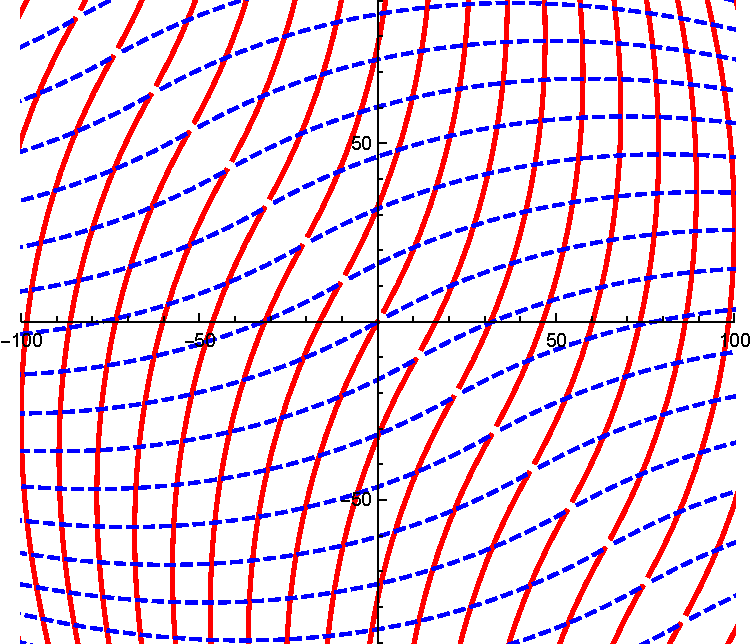
\includegraphics[width=.30\textwidth]{figures2/fig1575.pdf}
		\label{fig:wdispa_cs1}
	}\hspace{0.5 cm}
	\subfloat[][]
	{
		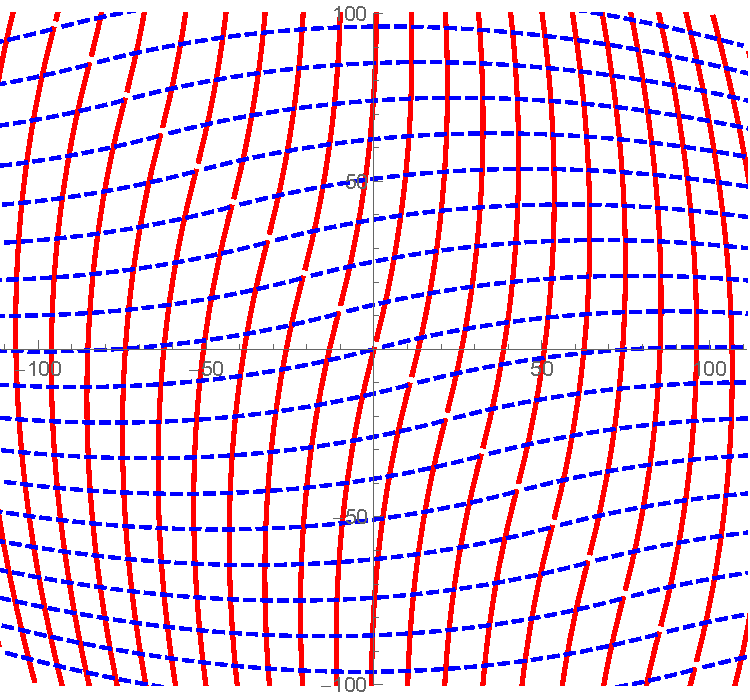
\includegraphics[width=.30\textwidth]{figures2/3060.pdf}
		\label{fig:wdispb_cs1}
	}
	
	\subfloat[][]
	{
		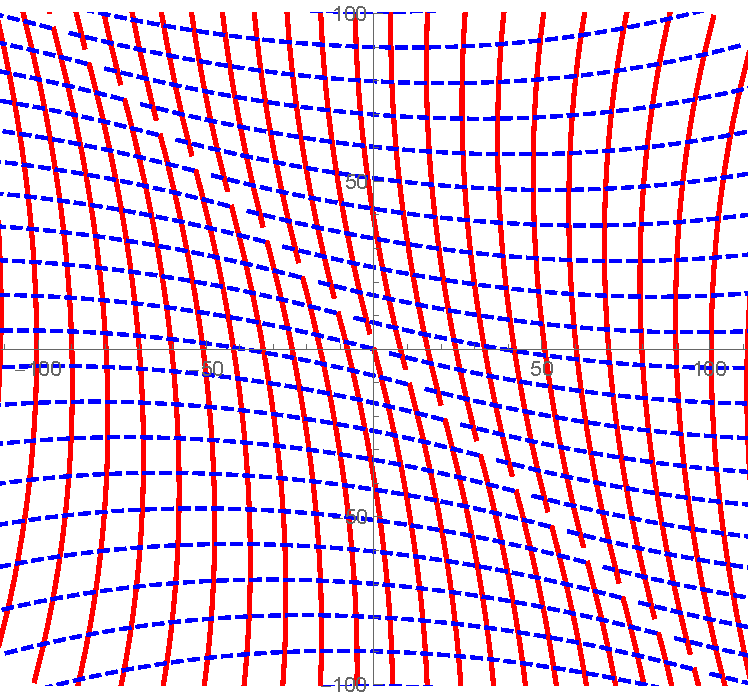
\includegraphics[width=.30\textwidth]{figures2/6030.pdf}
		\label{fig:wdispc_cs1}
	}\hspace{0.5 cm}
	\subfloat[][]
	{
		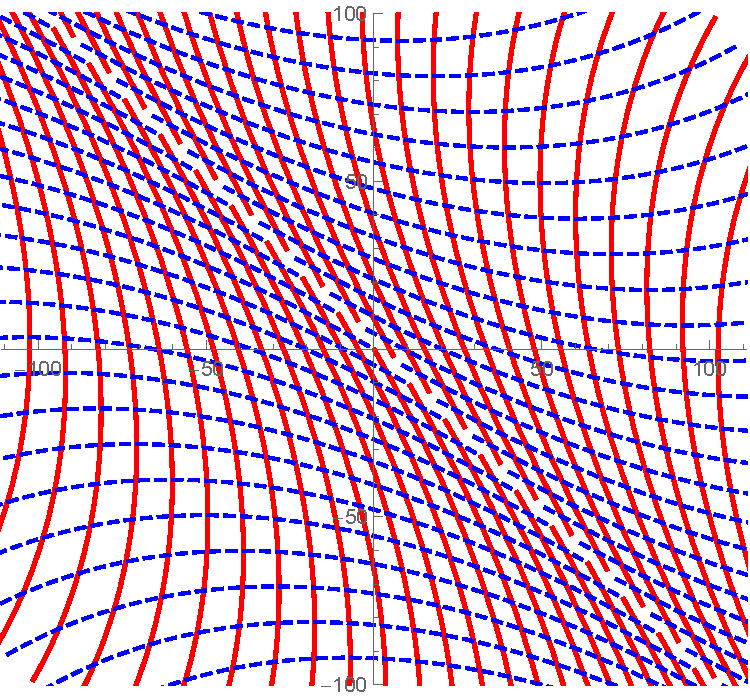
\includegraphics[width=.30\textwidth]{figures2/7515.pdf}
		\label{fig:wdispd_cs1}
	}
	\caption{Investigated VS composites a) VS-1 b) VS-2 c) VS-3 d) VS-4. All of them yield cylindrical bistable shapes similar to unsymmetric cross-ply laminate $[0_4/90_4]$}
	\label{fig:fiberpaths}
\end{figure}
\begin{table}[!h]
	\centering
	\setlength{\arrayrulewidth}{2pt}
	\begin{tabular}{lcccc}
		\hline
		{Type} & {$\phi$} & {$T_0$}  & {$T_1$} & {Layup}\\
		\hline
		{Straight} & {$45$}& {$45$} & {$45$} &{$\left[0_4/90_4\right]_{T}$}\\
		{VS-1}  & {$45$}& {$\pm 15$} & {$\pm 75$} & {$[45\langle{15|75 \rangle}_4/45\langle {-15|-75 \rangle}_4]_{T}$}\\
		{VS-2}  & {$45$}& {$\pm 30$} & {$\pm 60$} & {$[45\langle{30|60 \rangle}_4/45\langle {-30|-60 \rangle}_4]_{T}$}\\
		{VS-3} & {$45$} & {$\pm 60$} & {$\pm 30$} & {$[45\langle{60|30 \rangle}_4/45\langle {-60|-30 \rangle}_4]_{T}$}\\ 
		{VS-4} & {$45$} & {$\pm 75$} & {$\pm 15$} & {$[45\langle{75|15 \rangle}_4/45\langle {-75|-15 \rangle}_4]_{T}$}\\
		\hline
	\end{tabular}
	\vspace{5 mm}
	\caption{Fiber orientation and layup data for the investigated straight cross-ply and various VS composites}
	\label{data122}
\end{table}
\begin{figure}[!htb]
	\captionsetup[subfloat]{farskip=0.5pt,captionskip=2pt}
	\centering	
	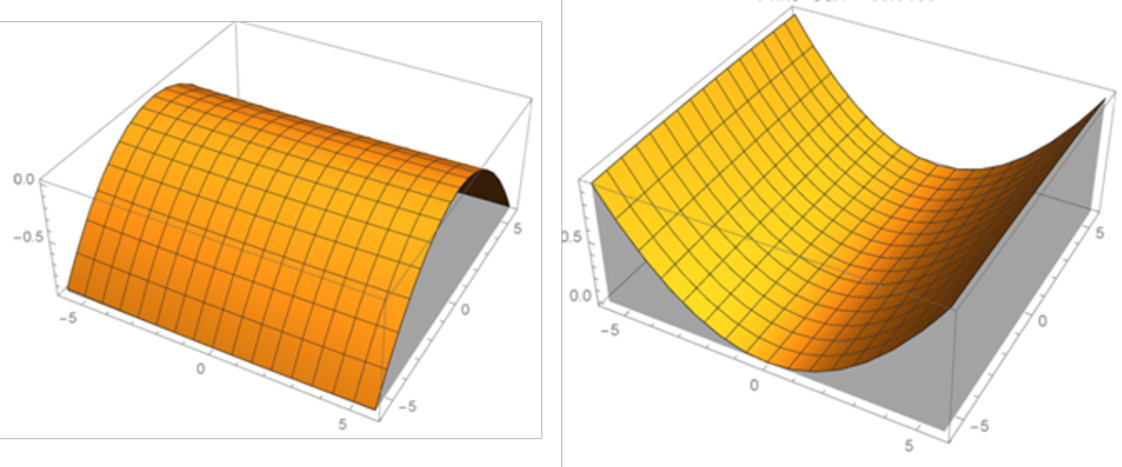
\includegraphics[width=.70\textwidth]{figures2/drawing.pdf}
	\label{fig:shapes}
\end{figure}


%phi=0\\
%plot here nxx \\
%nyy\\
%nxy\\
%comparison with FE\\
%Table for outof plane displacements with vs-1,vs-2 and vs-3 and vs-4. x=0 and y=0 planes\\
%Table with difference with FE\\
%Snap through load differentce\\
%vs-1
%nx=2,3,4,5
%Order 4
%change in difference with number of grid\\
%\section*{$\phi=0$}
%phi=0\\
%plot here nxx \\
%nyy\\
%nxy\\
%comparison with FE\\
%Figures for outof plane displacements with vs-1,vs-2 and vs-3 and vs-4. x=0 and y=0 planes\\
%Figure with difference with FE\\

%\begin{table}[!htb]
%	\centering
%	\setlength{\arrayrulewidth}{2pt}
%	%\begin{tabular}{|p{3cm}||p{3cm}|p{3cm}| }
%	\begin{tabular}{lccccccc}
%		\hline
%		% \multicolumn{3}{|c|}{Ord. 2} \\
%		% \hline
%		Order & n=2 & n=3 & n=4 & n= 5 & FE & Error(\%)\\
%		\hline
%		VS-1   & 10    & 10 & 10 & 10 & 10 & 0.1  \\
%		VS-2  & 10    & 10 & 10 & 10 & 10 & 0.1  \\
%		VS-3  & 10    & 10 & 10 & 10 & 10 & 0.1  \\
%		VS-4  & 10    & 10 & 10 & 10 & 10 & 0.1  \\
%		Straight [$0_4/90_4$]  & 10    & 10 & 10 & 10 & 10 & 0.1  \\
%		\hline
%	\end{tabular}
%	\vspace{5 mm}
%	\caption{Comparison between the snap-through loads with the formulated DQM method and FE}
%	\label{data122}
%\end{table}


% Please add the following required packages to your document preamble:
% \usepackage{booktabs}


\begin{table}[!h]
	\begin{tabular}{@{}llllllllll@{}}
		\hline
		\multirow{ 2}{*}{$T_0$}
		&
		\multirow{ 2}{*}{$T_1$}
		& \multicolumn{2}{l}{$n=2$}                                        & \multicolumn{2}{l}{$n=3$}                                                                            & \multicolumn{2}{l}{$n=4$}                                                                            & \multicolumn{2}{l}{$n=5$}                                                                            \\ \cline{3-10}

	{}	         & {}     &$w_1$ &$w_2$  &$w_1$ &$w_2$  &$w_1$  &$w_2$ &$w_1$  &$w_2$ \\ \hline
		15         & 75        & 0.06034
                                                 &  0.03474                                                & 0.05019                                                 & 0.03849                                                 & 0.04912                                                 & 0.03808                                                 & 0.04944                                                 & 0.03799                                                 \\
		30         & 60        & 0.06700                                                 & 0.05081                                                 &0.06433                                                  & 0.05200                                                  &0.06334                                                  & 0.05150                                                 &                                                  &                                                  \\ 
		60         & 30        & 0.06631                                                 &0.05175                                                  &0.06581                                                    & 0.05211                                                 &  0.06452                                             &  0.05021                                                & 0.6450                                                 &0.05022                                                  \\ 
		75         & 15        &0.06156                                                  &0.03411                                                  & 0.05314                                                  & 0.03858                                                  & 0.053212                                                 & 0.03413                                                 & 0.05315                                                 & 0.03365                                                 \\ 
		45         & 45        &                                                  &                                                  &                                                  &                                                  &                                                  &                                                  &                                                  &                                                  \\ \hline
	\end{tabular}
\label{disp}
\caption{Corner displacements-- in ($m$)}
\end{table}

\begin{table}[!h]
	\begin{tabular}{@{}lllllllllll@{}}
		\hline
		\multirow{ 2}{*}{$T_0$}
		&
		\multirow{ 2}{*}{$T_1$}
		& \multicolumn{2}{l}{$n=2$}                                        & \multicolumn{2}{l}{$n=3$}                                                                            & \multicolumn{2}{l}{$n=4$}                                                                            & 
		\multicolumn{2}{l}{$n=5$}    
	     & 
	    \multirow{ 2}{*}{FE}         \\ \cline{3-10}     
		
		{}	         & {}     &Force &Error  &Force &Error  &Force &Error  &Force &Error &{} \\ \hline
		15         & 75        & 1.97
		&  0.00                                                & 1.91                                                 & 0.0                                                 & 1.395                                                 & 0                                                & 1.3                                                & 0.0         &1.29                                        \\
		30         & 60        & 3.36                                                 & 0                                                 & 3.24                                                  & 0                                                  &2.75                                                  &0.0                                                 &                                                  &        &2.63                                           \\ 
		60         & 30        & 6.22                                                 &0                                                  &5.56                                                      & 0                                                 &  3.31                                             &  0.0                                                & 3.29                                                 &0.0   &3.17                                                \\ 
		75         & 15        &4.66                                                  &0.0                                                  & 4.20                                               &0.0                                                   & 2.15                                                 &0.0                                                 &1.83                                                  & 0.0   &2.0                                             \\ 
		45         & 45        & 4.98                                                 & 48.6                                                 &   4.32                                               & 28.9                                                 & 3.97                                                 & 18.5                                                 & 3.65                                                 &  8.96      &3.35                                          \\ \hline
	\end{tabular}
	\label{disp}
	\caption{Snap-through Loads-- in ($N$)}
\end{table}















%\begin{table}[!htb]
%	\centering
%	\setlength{\arrayrulewidth}{2pt}
%	%\begin{tabular}{|p{3cm}||p{3cm}|p{3cm}| }
%	\begin{tabular}{lcccccc}
%		\hline
%		% \multicolumn{3}{|c|}{Ord. 2} \\
%		% \hline
%		Order & n=12 & n=8 & n=32 & n=42 & Error(\%)\\
%		\hline
%		VS-1   & 10    & 10 & 10 & 10 & 0.1  \\
%		VS-2  & 10    & 10 & 10 & 10 & 0.1  \\
%		VS-3  & 10    & 10 & 10 & 10 & 0.1  \\
%		VS-4  & 10    & 10 & 10 & 10 & 0.1  \\
%		Straight [$0_4/90_4$]  & 10    & 10 & 10 & 10 & 0.1  \\
%		\hline
%	\end{tabular}
%	\vspace{5 mm}
%	\caption{Comparison between the snap-through loads with the formulated DQM method and FE, order 4}
%	\label{data122}
%\end{table}
\section*{$\phi=45$}
phi=45\\

\begin{figure}[!h]
	\centering 
	\setlength\fheight{4cm} 
	\setlength\fwidth{4cm} 
     % This file was created by matlab2tikz.
%
%The latest updates can be retrieved from
%  http://www.mathworks.com/matlabcentral/fileexchange/22022-matlab2tikz-matlab2tikz
%where you can also make suggestions and rate matlab2tikz.
%
%\definecolor{mycolor1}{rgb}{0.00000,0.44700,0.74100}%
%\definecolor{mycolor2}{rgb}{0.85000,0.32500,0.09800}%
%\definecolor{mycolor3}{rgb}{0.92900,0.69400,0.12500}%
%\definecolor{mycolor4}{rgb}{0.49400,0.18400,0.55600}%
%\definecolor{mycolor5}{rgb}{0.46600,0.67400,0.18800}%


\definecolor{mycolor1}{rgb}{0.0,0.0,0.6}%
\definecolor{mycolor2}{rgb}{0.25,0.37,1.0}%
\definecolor{mycolor3}{rgb}{0.4,0.7,1.0}%
\definecolor{mycolor4}{rgb}{0.8,0.9,1}%
\definecolor{mycolor5}{rgb}{0.80,0.0,0.0}%
%
\begin{tikzpicture}

\begin{axis}[%
width=3.521in,
height=2.866in,
at={(0.458in,0.381in)},
scale only axis,
xmin=-0.15,
xmax=0.15,
xlabel style={font=\color{white!15!black}},
xlabel={y [m]},
xtick={-0.15,-0.1,-0.05,0,0.05,0.1,0.15},
scaled x ticks = false,
x tick label style={/pgf/number format/fixed},
ymin=-0.01,
ymax=0.07,
ylabel style={font=\color{white!15!black}},
ylabel={w [m]},
scaled y ticks = false,
y tick label style={/pgf/number format/fixed},
xmajorgrids,
ymajorgrids,
axis background/.style={fill=white},
legend style={at={(0.3,0.627)}, anchor=south west, legend cell align=left, align=left, draw=white!15!black},
ticklabel style={font=\small}
]
\addplot [color=mycolor1,line width=1.5pt]
  table[row sep=crcr]{%
-0.125	0.0437058529577593\\
-0.1125	0.0354017172067955\\
-0.1	0.0279717104424978\\
-0.0875	0.021415829515137\\
-0.075	0.0157340716469815\\
-0.0625	0.0109264344322962\\
-0.05	0.00699291583734347\\
-0.0375	0.00393351420038257\\
-0.025	0.00174822823166989\\
-0.0125	0.000437057013458858\\
0	0\\
0.0125	0.000437057017540898\\
0.025	0.00174822826432621\\
0.0375	0.00393351431059765\\
0.05	0.00699291609859403\\
0.0625	0.0109264349425512\\
0.075	0.0157340725287021\\
0.0875	0.0214158309152768\\
0.1	0.0279717125325022\\
0.1125	0.0354017201826027\\
0.125	0.0437058570397993\\
};
\addlegendentry{VS-1}

\addplot [color=mycolor2,line width=1.5pt]
  table[row sep=crcr]{%
-0.125	0.05802197694348\\
-0.1125	0.0469845080470069\\
-0.1	0.0371141641848218\\
-0.0875	0.0284091832938236\\
-0.075	0.0208680106111517\\
-0.0625	0.014489298674185\\
-0.05	0.00927190732054271\\
-0.0375	0.00521490368808395\\
-0.025	0.00231756221490784\\
-0.0125	0.000579364639353476\\
0	-3.23604e-18\\
0.0125	0.000579364635666516\\
0.025	0.00231756218541216\\
0.0375	0.00521490358853603\\
0.05	0.00927190708457727\\
0.0625	0.014489298213315\\
0.075	0.0208680098147683\\
0.0875	0.0284091820291964\\
0.1	0.0371141622970982\\
0.1125	0.0469845053592131\\
0.125	0.05802197325652\\
};
\addlegendentry{VS-2}

\addplot [color=mycolor3,line width=1.5pt]
  table[row sep=crcr]{%
-0.125	0.05916281813648\\
-0.1125	0.0476700070234939\\
-0.1	0.0374871265978778\\
-0.0875	0.0285807898228126\\
-0.075	0.0209215375494797\\
-0.0625	0.01448383851706\\
-0.05	0.00924608935273472\\
-0.0375	0.00519061457168496\\
-0.025	0.00230366657709184\\
-0.0125	0.000575425660136483\\
0	3.23604e-18\\
0.0125	0.000575425663863523\\
0.025	0.00230366660690816\\
0.0375	0.00519061467231504\\
0.05	0.00924608959126528\\
0.0625	0.01448383898294\\
0.075	0.0209215383545203\\
0.0875	0.0285807911011874\\
0.1	0.0374871285061223\\
0.1125	0.0476700097405061\\
0.125	0.05916282186352\\
};
\addlegendentry{VS-3}

\addplot [color=mycolor4,line width=1.5pt]
  table[row sep=crcr]{%
-0.125	0.0455709334965\\
-0.1125	0.0361639725139485\\
-0.1	0.028044860670208\\
-0.0875	0.0211143836842995\\
-0.075	0.015284999555244\\
-0.0625	0.0104808385620625\\
-0.05	0.006637703263776\\
-0.0375	0.0037030684994055\\
-0.025	0.001636081387972\\
-0.0125	0.0004075613284965\\
0	0\\
0.0125	0.0004075613615035\\
0.025	0.001636081652028\\
0.0375	0.0037030693905945\\
0.05	0.006637705376224\\
0.0625	0.0104808426879375\\
0.075	0.015285006684756\\
0.0875	0.0211143950057005\\
0.1	0.028044877569792\\
0.1125	0.0361639965760515\\
0.125	0.0455709665035\\
};
\addlegendentry{VS-4}

\addplot [color=mycolor5,line width=1.5pt,dashed]
  table[row sep=crcr]{%
-0.125	0.065381211\\
-0.1125	0.0529784938071\\
-0.1	0.0418734867456\\
-0.0875	0.0320688028311\\
-0.075	0.0235667476656\\
-0.0625	0.0163693194375\\
-0.05	0.0104782089216\\
-0.0375	0.0058947994791\\
-0.025	0.0026201670576\\
-0.0125	0.0006550801911\\
0	0\\
0.0125	0.0006550801911\\
0.025	0.0026201670576\\
0.0375	0.0058947994791\\
0.05	0.0104782089216\\
0.0625	0.0163693194375\\
0.075	0.0235667476656\\
0.0875	0.0320688028311\\
0.1	0.0418734867456\\
0.1125	0.0529784938071\\
0.125	0.065381211\\
};
\addlegendentry{Straight[$0_4/90_4]$}
\end{axis}
\end{tikzpicture}% 
     \label{plotx0}
\end{figure}


\begin{figure}[!h]
	\centering 
	\setlength\fheight{8cm} 
	\setlength\fwidth{8cm} 
	% This file was created by matlab2tikz.
%
%The latest updates can be retrieved from
%  http://www.mathworks.com/matlabcentral/fileexchange/22022-matlab2tikz-matlab2tikz
%where you can also make suggestions and rate matlab2tikz.
%
\definecolor{mycolor1}{rgb}{0.0,0.0,0.6}%
\definecolor{mycolor2}{rgb}{0.25,0.37,1.0}%
\definecolor{mycolor3}{rgb}{0.4,0.7,1.0}%
\definecolor{mycolor4}{rgb}{0.8,0.9,1}%
\definecolor{mycolor5}{rgb}{0.80,0.0,0.0}%}%
%
\begin{tikzpicture}

\begin{axis}[%
width=3.521in,
height=2.866in,
at={(1.23in,0.795in)},
scale only axis,
xmin=-0.15,
xmax=0.15,
xtick={-0.15,-0.1,-0.05,0,0.05,0.1,0.15},
scaled x ticks = false,
x tick label style={/pgf/number format/fixed},
xlabel style={font=\color{white!15!black}},
xlabel={y [m]},
ymin=-0.001,
ymax=0.005,
ylabel style={font=\color{white!15!black}},
ylabel={w [m]},
xmajorgrids,
ymajorgrids,
axis background/.style={fill=white},
legend style={at={(0.573,0.67)}, anchor=south west, legend cell align=left, align=left, draw=white!15!black}
]
\addplot [color=mycolor1,line width=1.5pt]
  table[row sep=crcr]{%
0.125	0.00196467704102\\
0.122395836	0.00184140167452469\\
0.119791664	0.00171853023889577\\
0.1171875	0.00159674039749268\\
0.114583336	0.00147619591942253\\
0.111979164	0.00135746394605775\\
0.109375	0.00124092999891574\\
0.106770836	0.00112696683515832\\
0.104166664	0.00101595057960977\\
0.1015625	0.000908374618849718\\
0.0989583358	0.00080442058186574\\
0.0963541642	0.000704574021639391\\
0.09375	0.000609135529024068\\
0.0911458358	0.000518496165240717\\
0.0885416642	0.000432950314239837\\
0.0859375	0.000352706499337187\\
0.0833333358	0.000278064732503469\\
0.0807291642	0.000209128345062128\\
0.078125	0.000146013797856445\\
0.0755208358	8.89300510375779e-05\\
0.0729166642	3.76893810263221e-05\\
0.0703125	-7.48380918186471e-06\\
0.0677083358	-4.68716136044038e-05\\
0.0651041642	-8.04528127785753e-05\\
0.0625	-0.000108395057372498\\
0.0598958321	-0.000131072745755974\\
0.0572916679	-0.000148600779975831\\
0.0546875	-0.000161336184141268\\
0.0520833321	-0.00016958942287335\\
0.0494791679	-0.0001737083096626\\
0.046875	-0.000174100928745039\\
0.0442708321	-0.000171139298229608\\
0.0416666679	-0.000165252784140407\\
0.0390625	-0.000156870532271728\\
0.0364583321	-0.000146416113486313\\
0.0338541679	-0.000134310445754578\\
0.03125	-0.000120993737640312\\
0.028645834	-0.000106880807188479\\
0.026041666	-9.23753158333044e-05\\
0.0234375	-7.78767896008204e-05\\
0.020833334	-6.3752817881698e-05\\
0.018229166	-5.03530028102587e-05\\
0.015625	-3.8003434734336e-05\\
0.013020833	-2.70010771614102e-05\\
0.010416667	-1.76075567917996e-05\\
0.0078125	-1.00509214529981e-05\\
0.00520833349	-4.51443033324352e-06\\
0.00260416674	-1.1359914681238e-06\\
0	0\\
-0.00260416674	-1.13599150503461e-06\\
-0.00520833349	-4.51443062852999e-06\\
-0.0078125	-1.00509224495899e-05\\
-0.010416667	-1.76075591540915e-05\\
-0.013020833	-2.70010817752607e-05\\
-0.015625	-3.80034427070704e-05\\
-0.018229166	-5.03520154706643e-05\\
-0.020833334	-6.37528367800331e-05\\
-0.0234375	-7.78768165087989e-05\\
-0.026041666	-9.23753527441087e-05\\
-0.028645834	-0.000106880856316768\\
-0.03125	-0.000120993801422187\\
-0.0338541679	-0.00013431052684763\\
-0.0364583321	-0.000146416214769558\\
-0.0390625	-0.000156870656845703\\
-0.0416666679	-0.000165252935327086\\
-0.0442708321	-0.000171139479572389\\
-0.046875	-0.000174101144008867\\
-0.0494791679	-0.000173708562833846\\
-0.0520833321	-0.000169579718159787\\
-0.0546875	-0.000161326525972255\\
-0.0572916679	-0.000148601173002133\\
-0.0598958321	-0.000131073194849739\\
-0.0625	-0.0001083955676275\\
-0.0651041642	-8.04533895098734e-05\\
-0.0677083358	-4.68722623488231e-05\\
-0.0703125	-7.48453569728545e-06\\
-0.0729166642	3.76885707603636e-05\\
-0.0755208358	8.89291508198095e-05\\
-0.078125	0.000146012801264649\\
-0.0807291642	0.00020912724545237\\
-0.0833333358	0.000278063523010026\\
-0.0859375	0.000352705172873505\\
-0.0885416642	0.000432948863497588\\
-0.0911458358	0.000518494582689724\\
-0.09375	0.00060913380691344\\
-0.0963541642	0.000704572151996416\\
-0.0989583358	0.000804418556495771\\
-0.1015625	0.000908372429337542\\
-0.104166664	0.00101594821731829\\
-0.106770836	0.00112696429122838\\
-0.109375	0.00124092726426785\\
-0.111979164	0.00135746101139041\\
-0.114583336	0.0014761927752121\\
-0.1171875	0.00159673703399536\\
-0.119791664	0.00171862664614567\\
-0.122395836	0.00184139784233369\\
-0.125	0.00196467295898\\
};
\addlegendentry{VS-1}

\addplot [color=mycolor2,line width=1.5pt]
  table[row sep=crcr]{%
0.125	0.00447207325652\\
0.122395836	0.00415036202541097\\
0.119791664	0.00384546623247121\\
0.1171875	0.00355658212722137\\
0.114583336	0.00328328465948087\\
0.111979164	0.00302504979242132\\
0.109375	0.00278137401283957\\
0.106770836	0.00255193390930025\\
0.104166664	0.0023361070830939\\
0.1015625	0.00213349025923296\\
0.0989583358	0.00194386151750767\\
0.0963541642	0.00176660068119003\\
0.09375	0.00160140384376625\\
0.0911458358	0.00144775131102851\\
0.0885416642	0.00130522435379029\\
0.0859375	0.00117351937531051\\
0.0833333358	0.0010519182838575\\
0.0807291642	0.000940203952261479\\
0.078125	0.000837773094243158\\
0.0755208358	0.000744109220197499\\
0.0729166642	0.000658796804661868\\
0.0703125	0.000581232872447948\\
0.0677083358	0.00051100253575774\\
0.0651041642	0.000447691870556108\\
0.0625	0.000390598213314997\\
0.0598958321	0.000339506633188822\\
0.0572916679	0.00029381131398575\\
0.0546875	0.000253000251740743\\
0.0520833321	0.000216836695089638\\
0.0494791679	0.000184813996874932\\
0.046875	0.000156581754128004\\
0.0442708321	0.000131784172276573\\
0.0416666679	0.000110105561084867\\
0.0390625	9.12371183859209e-05\\
0.0364583321	7.4894006499222e-05\\
0.0338541679	6.08314921906068e-05\\
0.03125	4.88123739299964e-05\\
0.028645834	3.86231746947333e-05\\
0.026041666	3.00585403006032e-05\\
0.0234375	2.29351816820747e-05\\
0.020833334	1.70889641464467e-05\\
0.018229166	1.2356298057349e-05\\
0.015625	8.59983407034825e-06\\
0.013020833	5.67762837879349e-06\\
0.010416667	3.4737457042691e-06\\
0.0078125	1.88125502935955e-06\\
0.00520833349	8.12805148231037e-07\\
0.00260416674	1.99377393106199e-07\\
0	-3.23604e-18\\
-0.00260416674	1.99377426444596e-07\\
-0.00520833349	8.12805414938239e-07\\
-0.0078125	1.88125592949628e-06\\
-0.010416667	3.47374783792672e-06\\
-0.013020833	5.67763254609281e-06\\
-0.015625	8.59984127144192e-06\\
-0.018229166	1.23563094924181e-05\\
-0.020833334	1.70889812157076e-05\\
-0.0234375	2.29352059857657e-05\\
-0.026041666	3.00585736389978e-05\\
-0.028645834	3.86232190681427e-05\\
-0.03125	4.88124315387467e-05\\
-0.0338541679	6.08315654350728e-05\\
-0.0364583321	7.48940979797743e-05\\
-0.0390625	9.12372309030103e-05\\
-0.0416666679	0.000110105697638953\\
-0.0442708321	0.000131784336068104\\
-0.046875	0.000156581948557536\\
-0.0494791679	0.000184814225543013\\
-0.0520833321	0.000216836961796795\\
-0.0546875	0.000253000560487639\\
-0.0572916679	0.000293811668973026\\
-0.0598958321	0.000339507038817072\\
-0.0625	0.000390598674184995\\
-0.0651041642	0.000447692391468505\\
-0.0677083358	0.000511003121713469\\
-0.0703125	0.000581233528647619\\
-0.0729166642	0.000658797536506286\\
-0.0755208358	0.00074411003328774\\
-0.078125	0.000837773994379881\\
-0.0807291642	0.000940204945445569\\
-0.0833333358	0.00105191937629019\\
-0.0859375	0.00117352057339248\\
-0.0885416642	0.00130522566412254\\
-0.0911458358	0.0014477527404124\\
-0.09375	0.0016014053992025\\
-0.0963541642	0.00176660236987972\\
-0.0989583358	0.00194386334685234\\
-0.1015625	0.00213349223683333\\
-0.104166664	0.00233610921675114\\
-0.106770836	0.00255193620701609\\
-0.109375	0.00278137648281472\\
-0.111979164	0.00302505244305706\\
-0.114583336	0.00328328749937908\\
-0.1171875	0.00355658516518279\\
-0.119791664	0.00384546947749721\\
-0.122395836	0.00415046548670359\\
-0.125	0.00447207694348\\
};
\addlegendentry{VS-2}

\addplot [color=mycolor3,line width=1.5pt]
  table[row sep=crcr]{%
0.125	0.00495492186351999\\
0.122395836	0.00457218539731492\\
0.119791664	0.00421455053892907\\
0.1171875	0.00388098824661377\\
0.114583336	0.00357015424715344\\
0.111979164	0.0032809123723952\\
0.109375	0.0030121547200925\\
0.106770836	0.00276275974586396\\
0.104166664	0.00253141399852543\\
0.1015625	0.00231703073313072\\
0.0989583358	0.00211851097420121\\
0.0963541642	0.00193466457882393\\
0.09375	0.0017646250830475\\
0.0911458358	0.00160711682649615\\
0.0885416642	0.00146147217027313\\
0.0859375	0.00132664591530643\\
0.0833333358	0.00120188506697206\\
0.0807291642	0.00108644464342029\\
0.078125	0.000979700723515629\\
0.0755208358	0.000881022971762679\\
0.0729166642	0.000789789057492454\\
0.0703125	0.00070559634942776\\
0.0677083358	0.000628137165146272\\
0.0651041642	0.000556811819861214\\
0.0625	0.000491438982940004\\
0.0598958321	0.000431531966400405\\
0.0572916679	0.000377020265577335\\
0.0546875	0.000327434162094086\\
0.0520833321	0.000282546222531108\\
0.0494791679	0.000242186119746206\\
0.046875	0.000206066773076254\\
0.0442708321	0.000173922727064429\\
0.0416666679	0.000145525634991314\\
0.0390625	0.000120611050217289\\
0.0364583321	9.89254971406088e-05\\
0.0338541679	8.02226109785078e-05\\
0.03125	6.4230575992503e-05\\
0.028645834	5.06983000078654e-05\\
0.026041666	3.93698302857981e-05\\
0.0234375	2.99982810217409e-05\\
0.020833334	2.23429351319286e-05\\
0.018229166	1.61806292237679e-05\\
0.015625	1.12934440693783e-05\\
0.013020833	7.49288053926607e-06\\
0.010416667	4.61145316036184e-06\\
0.0078125	2.51369204431963e-06\\
0.00520833349	1.09161405023145e-06\\
0.00260416674	2.69278479743101e-07\\
0	3.23604e-18\\
-0.00260416674	2.69278446042289e-07\\
-0.00520833349	1.09161378062495e-06\\
-0.0078125	2.51369113439775e-06\\
-0.010416667	4.61145100350978e-06\\
-0.013020833	7.4928763266651e-06\\
-0.015625	1.12934367900033e-05\\
-0.018229166	1.61806176643912e-05\\
-0.020833334	2.23429178771121e-05\\
-0.0234375	2.99982564538506e-05\\
-0.026041666	3.93697965849903e-05\\
-0.028645834	5.0698255152084e-05\\
-0.03125	6.42305177575029e-05\\
-0.0338541679	8.02225369378193e-05\\
-0.0364583321	9.8925404665595e-05\\
-0.0390625	0.000120610936477055\\
-0.0416666679	0.000145525496952784\\
-0.0442708321	0.000173922561492363\\
-0.046875	0.000206066576533128\\
-0.0494791679	0.000242185888592332\\
-0.0520833321	0.000282545952924646\\
-0.0546875	0.000327433849990882\\
-0.0572916679	0.000377019906731084\\
-0.0598958321	0.000431531556362672\\
-0.0625	0.000491438517060003\\
-0.0651041642	0.000556811293286115\\
-0.0677083358	0.000628136572820771\\
-0.0703125	0.000705595686094712\\
-0.0729166642	0.000789788317692344\\
-0.0755208358	0.000881022149833537\\
-0.078125	0.000979699813593755\\
-0.0807291642	0.00108644363943954\\
-0.0833333358	0.00120188396266381\\
-0.0859375	0.00132664470420041\\
-0.0885416642	0.0014614708456966\\
-0.0911458358	0.00160711538157379\\
-0.09375	0.00176462351070249\\
-0.0963541642	0.00193466287177693\\
-0.0989583358	0.00211850912497022\\
-0.1015625	0.00231702873403236\\
-0.104166664	0.00253141184167375\\
-0.106770836	0.00276275742317025\\
-0.109375	0.00301215222326687\\
-0.111979164	0.00328090969294508\\
-0.114583336	0.00357015137638343\\
-0.1171875	0.00388098517562745\\
-0.119791664	0.00421454725862724\\
-0.122395836	0.00457218189839547\\
-0.125	0.00495491813648\\
};
\addlegendentry{VS-3}

\addplot [color=mycolor4,line width=1.5pt]
  table[row sep=crcr]{%
0.125	0.0033314665035\\
0.122395836	0.00310689268060334\\
0.119791664	0.00290133692003099\\
0.1171875	0.00271328912718201\\
0.114583336	0.00254134256783559\\
0.111979164	0.0023839132038979\\
0.109375	0.00223935584365332\\
0.106770836	0.0021062302529388\\
0.104166664	0.0019829188584581\\
0.1015625	0.00186824142427112\\
0.0989583358	0.00176062407095406\\
0.0963541642	0.00165921613606749\\
0.09375	0.00156280168897657\\
0.0911458358	0.00147077377273287\\
0.0885416642	0.00138254798232587\\
0.0859375	0.0012974735062948\\
0.0833333358	0.00121540977843433\\
0.0807291642	0.00113603875860954\\
0.078125	0.00105937479333497\\
0.0755208358	0.000985243687466575\\
0.0729166642	0.000913793748312625\\
0.0703125	0.00084500451579016\\
0.0677083358	0.00077886814782171\\
0.0651041642	0.000715599283413217\\
0.0625	0.000655172687937499\\
0.0598958321	0.000597615637988028\\
0.0572916679	0.000542963904446084\\
0.0546875	0.000491220372638062\\
0.0520833321	0.000442373511615845\\
0.0494791679	0.000396403550265506\\
0.046875	0.000353239681336915\\
0.0442708321	0.000312856166423402\\
0.0416666679	0.00027518903426288\\
0.0390625	0.000240163774063111\\
0.0364583321	0.00020774044558225\\
0.0338541679	0.000177860881908747\\
0.03125	0.000150476859429688\\
0.028645834	0.000125544528002332\\
0.026041666	0.000103020406769659\\
0.0234375	8.2864194633667e-05\\
0.020833334	6.50467001802565e-05\\
0.018229166	4.95038315610071e-05\\
0.015625	3.61920854560548e-05\\
0.013020833	2.50512508613551e-05\\
0.010416667	1.60205412724183e-05\\
0.0078125	9.03588626184084e-06\\
0.00520833349	4.04990733890343e-06\\
0.00260416674	1.02650308554817e-06\\
0	3.18524e-38\\
-0.00260416674	1.02650278709075e-06\\
-0.00520833349	4.04990495124408e-06\\
-0.0078125	9.03587820349122e-06\\
-0.010416667	1.60205221711433e-05\\
-0.013020833	2.50512135541838e-05\\
-0.015625	3.61920209892579e-05\\
-0.018229166	4.95037291901325e-05\\
-0.020833334	6.50465473700566e-05\\
-0.0234375	8.28639770582276e-05\\
-0.026041666	0.000103020108312289\\
-0.028645834	0.000125544130755514\\
-0.03125	0.000150476343695312\\
-0.0338541679	0.000177860226197783\\
-0.0364583321	0.000207739626615248\\
-0.0390625	0.000240162766769409\\
-0.0416666679	0.00027518781178129\\
-0.0442708321	0.000312854700102353\\
-0.046875	0.000353247940733399\\
-0.0494791679	0.000396401503146094\\
-0.0520833321	0.000442371123956872\\
-0.0546875	0.000491217608624146\\
-0.0572916679	0.000542960726471559\\
-0.0598958321	0.000597612006657153\\
-0.0625	0.0006551685620625\\
-0.0651041642	0.000715594620016982\\
-0.0677083358	0.000778862902133999\\
-0.0703125	0.000844998641253297\\
-0.0729166642	0.0009137871965766\\
-0.0755208358	0.000985236408388506\\
-0.078125	0.00105936673498535\\
-0.0807291642	0.00113602986726617\\
-0.0833333358	0.00121539999858161\\
-0.0859375	0.00129746278063147\\
-0.0885416642	0.00138253625175748\\
-0.0911458358	0.0014708609763711\\
-0.09375	0.00156278776414844\\
-0.0963541642	0.00165920101830633\\
-0.0989583358	0.00176060769399877\\
-0.1015625	0.00186822372007703\\
-0.104166664	0.00198289975718641\\
-0.106770836	0.00210620968295527\\
-0.109375	0.00223933373154199\\
-0.111979164	0.00238388947444765\\
-0.114583336	0.00254131714403926\\
-0.1171875	0.00271326193025208\\
-0.119791664	0.00290130786938413\\
-0.122395836	0.0031068616938594\\
-0.125	0.0033314334965\\
};
\addlegendentry{VS-4}

\end{axis}
\end{tikzpicture}% 
	\label{plotx0diff}
\end{figure}

\begin{figure}[!h]
	\centering 
	\setlength\fheight{8cm} 
	\setlength\fwidth{8cm} 
	% This file was created by matlab2tikz.
%
%The latest updates can be retrieved from
%  http://www.mathworks.com/matlabcentral/fileexchange/22022-matlab2tikz-matlab2tikz
%where you can also make suggestions and rate matlab2tikz.
%
\definecolor{mycolor1}{rgb}{0.0,0.0,0.6}%
\definecolor{mycolor2}{rgb}{0.25,0.37,1.0}%
\definecolor{mycolor3}{rgb}{0.4,0.7,1.0}%
\definecolor{mycolor4}{rgb}{0.8,0.9,1}%
\definecolor{mycolor5}{rgb}{0.80,0.0,0.0}%
%
\begin{tikzpicture}

\begin{axis}[%
width=3.521in,
height=2.866in,
at={(0.758in,0.481in)},
scale only axis,
xmin=-0.15,
xmax=0.15,
xtick={-0.15,-0.1,-0.05,0,0.05,0.1,0.15},
scaled x ticks = false,
x tick label style={/pgf/number format/fixed},
xlabel style={font=\color{white!15!black}},
xlabel={x [m]},
ymin=-0.0003,
ymax=0.0004,
ylabel style={font=\color{white!15!black}},
ylabel={w [m]},
xmajorgrids,
ymajorgrids,
axis background/.style={fill=white},
legend style={at={(0.323,0.668)}, anchor=south west, legend cell align=left, align=left, draw=white!15!black}
]
\addplot [color=mycolor1,line width=1.5pt]
  table[row sep=crcr]{%
-0.125	-0.00029127444232\\
-0.11875	-0.00027440353227161\\
-0.1125	-0.00025609523605128\\
-0.10625	-0.00023671311642727\\
-0.1	-0.00021660108406784\\
-0.09375	-0.00019608339754125\\
-0.0875	-0.00017546466331576\\
-0.08125	-0.00015502983575963\\
-0.075	-0.00013504421714112\\
-0.06875	-0.00011575345762849\\
-0.0625	-9.738355529e-05\\
-0.05625	-8.014085609391e-05\\
-0.05	-6.421205390848e-05\\
-0.04375	-4.976419050197e-05\\
-0.0375	-3.694465554264e-05\\
-0.03125	-2.588118659875e-05\\
-0.025	-1.668186913856e-05\\
-0.01875	-9.43513653032999e-06\\
-0.0125	-4.20977004232e-06\\
-0.00624999999999999	-1.05489884279e-06\\
0	0\\
0.00624999999999999	-1.05489848221e-06\\
0.0125	-4.20976715768e-06\\
0.01875	-9.43512679466999e-06\\
0.025	-1.668184606144e-05\\
0.03125	-2.588114152625e-05\\
0.0375	-3.694457765736e-05\\
0.04375	-4.976406682303e-05\\
0.05	-6.421186929152e-05\\
0.05625	-8.014059323109e-05\\
0.0625	-9.738319471e-05\\
0.06875	-0.00011575297769651\\
0.075	-0.00013504359405888\\
0.08125	-0.00015502904356537\\
0.0875	-0.00017546367388424\\
0.09375	-0.00019608218058375\\
0.1	-0.00021659960713216\\
0.10625	-0.00023671134489773\\
0.1125	-0.00025609313314872\\
0.11875	-0.00027440105905339\\
0.125	-0.00029127155768\\
};
\addlegendentry{VS-1}

\addplot [color=mycolor2,line width=1.5pt]
  table[row sep=crcr]{%
-0.125	-0.000232454323495003\\
-0.11875	-0.000221773838300279\\
-0.1125	-0.000209247543927858\\
-0.10625	-0.00019525336536012\\
-0.1	-0.000180148799229443\\
-0.09375	-0.000164270913818206\\
-0.0875	-0.000147936349058788\\
-0.08125	-0.000131441316533568\\
-0.075	-0.000115061599474923\\
-0.06875	-9.90525527652339e-05\\
-0.0625	-8.36491029368782e-05\\
-0.05625	-6.90657481722351e-05\\
-0.05	-5.54965583036832e-05\\
-0.04375	-4.31151748136014e-05\\
-0.0375	-3.20748108343682e-05\\
-0.03125	-2.25082511483626e-05\\
-0.025	-1.45278521879632e-05\\
-0.01875	-8.22554203554885e-06\\
-0.0125	-3.67282042349823e-06\\
-0.00624999999999999	-9.20758734190109e-07\\
0	-3.23604e-18\\
0.00624999999999999	-9.20758903316359e-07\\
0.0125	-3.67282177650823e-06\\
0.01875	-8.2255466019576e-06\\
0.025	-1.45278630120432e-05\\
0.03125	-2.25082722891439e-05\\
0.0375	-3.20748473656382e-05\\
0.04375	-4.31152328239051e-05\\
0.05	-5.54966448963232e-05\\
0.05625	-6.90658714652714e-05\\
0.0625	-8.36492720631283e-05\\
0.06875	-9.90527778722726e-05\\
0.075	-0.000115061891725083\\
0.08125	-0.000131441688103939\\
0.0875	-0.000147936813141218\\
0.09375	-0.0001642714846193\\
0.1	-0.000180149491970563\\
0.10625	-0.000195254196277386\\
0.1125	-0.000209248530272148\\
0.11875	-0.000221774998337228\\
0.125	-0.000232455676505003\\
};
\addlegendentry{VS-2}

\addplot [color=mycolor3,line width=1.5pt]
  table[row sep=crcr]{%
-0.125	0.000322042564041003\\
-0.11875	0.000289240474230281\\
-0.1125	0.000258400752455892\\
-0.10625	0.000229479155052307\\
-0.1	0.000202433829908995\\
-0.09375	0.000177225316470425\\
-0.0875	0.000153816545736066\\
-0.08125	0.000132172840260388\\
-0.075	0.000112261914152859\\
-0.06875	9.40538730779496e-05\\
-0.0625	7.75212142551282e-05\\
-0.05625	6.26388264588644e-05\\
-0.05	4.93839900186272e-05\\
-0.04375	3.77363768188861e-05\\
-0.0375	2.76780502991102e-05\\
-0.03125	1.91934654537689e-05\\
-0.025	1.22694688323312e-05\\
-0.01875	6.8952985392666e-06\\
-0.0125	3.06258423404423e-06\\
-0.00624999999999999	7.65347131133359e-07\\
0	3.23604e-18\\
0.00624999999999999	7.65347165123109e-07\\
0.0125	3.06258450596223e-06\\
0.01875	6.89529945698985e-06\\
0.025	1.22694710076752e-05\\
0.03125	1.91934697024876e-05\\
0.0375	2.76780576408962e-05\\
0.04375	3.77363884773704e-05\\
0.05	4.93840074213792e-05\\
0.05625	6.26388512373921e-05\\
0.0625	7.75212482448782e-05\\
0.06875	9.40539183183069e-05\\
0.075	0.000112261972887147\\
0.08125	0.000132172914935869\\
0.0875	0.00015381663900394\\
0.09375	0.000177225431185831\\
0.1	0.000202433969131011\\
0.10625	0.000229479322043949\\
0.1125	0.000258400950684114\\
0.11875	0.000289240707365976\\
0.125	0.000322042835959003\\
};
\addlegendentry{VS-3}

\addplot [color=mycolor4,line width=1.5pt]
  table[row sep=crcr]{%
-0.125	0.00020496195179\\
-0.11875	0.000125323155084701\\
-0.1125	6.16833035549101e-05\\
-0.10625	1.21610958117837e-05\\
-0.1	-2.502307748352e-05\\
-0.09375	-5.15471336198437e-05\\
-0.0875	-6.898729783603e-05\\
-0.08125	-7.88181033209212e-05\\
-0.075	-8.241239121336e-05\\
-0.06875	-8.10413106021888e-05\\
-0.0625	-7.587431852625e-05\\
-0.05625	-6.79791799743862e-05\\
-0.05	-5.832196788544e-05\\
-0.04375	-4.77670631482537e-05\\
-0.0375	-3.707715460167e-05\\
-0.03125	-2.69132390345313e-05\\
-0.025	-1.783462118568e-05\\
-0.01875	-1.02989137439587e-05\\
-0.0125	-4.66203734821e-06\\
-0.00624999999999999	-1.17822058727625e-06\\
0	0\\
0.00624999999999999	-1.17822007522375e-06\\
0.0125	-4.66203325179e-06\\
0.01875	-1.02988999185412e-05\\
0.025	-1.783458841432e-05\\
0.03125	-2.69131750279688e-05\\
0.0375	-3.707704399833e-05\\
0.04375	-4.77668875142462e-05\\
0.05	-5.832170571456e-05\\
0.05625	-6.79788066881137e-05\\
0.0625	-7.587380647375e-05\\
0.06875	-8.10406290603112e-05\\
0.075	-8.241150638664e-05\\
0.08125	-7.88169783415787e-05\\
0.0875	-6.898589276397e-05\\
0.09375	-5.15454054426562e-05\\
0.1	-2.502098011648e-05\\
0.10625	1.21636115257162e-05\\
0.1125	6.16862898450901e-05\\
0.11875	0.000125326667252799\\
0.125	0.00020496604821\\
};
\addlegendentry{VS-4}

\addplot [color=mycolor5, line width=1.5pt, dashed]
  table[row sep=crcr]{%
-0.125	-3.22950000000014e-05\\
-0.11875	-1.69370166937512e-05\\
-0.1125	-4.80517110000102e-06\\
-0.10625	4.48557080624917e-06\\
-0.1	1.12994303999993e-05\\
-0.09375	1.59798164062494e-05\\
-0.0875	1.88493248999995e-05\\
-0.08125	2.02097393062496e-05\\
-0.075	2.03420303999997e-05\\
-0.06875	1.95063563062498e-05\\
-0.0625	1.79420624999998e-05\\
-0.05625	1.58676818062499e-05\\
-0.05	1.34809343999999e-05\\
-0.04375	1.09587278062499e-05\\
-0.0375	8.45715689999996e-06\\
-0.03125	6.11150390624998e-06\\
-0.025	4.03623839999999e-06\\
-0.01875	2.32501730624999e-06\\
-0.0125	1.0506849e-06\\
-0.00624999999999999	2.65272806249999e-07\\
0	0\\
0.00624999999999999	2.65272806249999e-07\\
0.0125	1.0506849e-06\\
0.01875	2.32501730625e-06\\
0.025	4.03623840000001e-06\\
0.03125	6.11150390625002e-06\\
0.0375	8.45715690000003e-06\\
0.04375	1.09587278062501e-05\\
0.05	1.34809344000001e-05\\
0.05625	1.58676818062501e-05\\
0.0625	1.79420625000002e-05\\
0.06875	1.95063563062502e-05\\
0.075	2.03420304000003e-05\\
0.08125	2.02097393062504e-05\\
0.0875	1.88493249000005e-05\\
0.09375	1.59798164062506e-05\\
0.1	1.12994304000007e-05\\
0.10625	4.48557080625085e-06\\
0.1125	-4.80517109999902e-06\\
0.11875	-1.69370166937488e-05\\
0.125	-3.22949999999986e-05\\
};
\addlegendentry{Straight[$0_4/90_4]$}

\end{axis}
\end{tikzpicture}% 
	\label{ploty0}
\end{figure}

\begin{figure}[!h]
	\centering 
	\setlength\fheight{8cm} 
	\setlength\fwidth{8cm} 
	% This file was created by matlab2tikz.
%
%The latest updates can be retrieved from
%  http://www.mathworks.com/matlabcentral/fileexchange/22022-matlab2tikz-matlab2tikz
%where you can also make suggestions and rate matlab2tikz.
%
\definecolor{mycolor1}{rgb}{0.0,0.0,0.6}%
\definecolor{mycolor2}{rgb}{0.25,0.37,1.0}%
\definecolor{mycolor3}{rgb}{0.4,0.7,1.0}%
\definecolor{mycolor4}{rgb}{0.8,0.9,1}%
\definecolor{mycolor5}{rgb}{0.80,0.0,0.0}%
%
\begin{tikzpicture}

\begin{axis}[%
width=3.521in,
height=2.866in,
at={(0.758in,0.481in)},
scale only axis,
xmin=-0.15,
xmax=0.15,
xtick={-0.15,-0.1,-0.05,0,0.05,0.1,0.15},
scaled x ticks = false,
x tick label style={/pgf/number format/fixed},
xlabel style={font=\color{white!15!black}},
xlabel={x [m]},
ymin=-0.0003,
ymax=0.0004,
ylabel style={font=\color{white!15!black}},
ylabel={w [m]},
xmajorgrids,
ymajorgrids,
axis background/.style={fill=white},
legend style={at={(0.323,0.668)}, anchor=south west, legend cell align=left, align=left, draw=white!15!black}
]
\addplot [color=mycolor1,line width=1.5pt]
  table[row sep=crcr]{%
0.125	0.00015253444232\\
0.122395836	4.24489892677289e-05\\
0.119791664	-1.81367287113392e-05\\
0.1171875	-4.37602987780762e-05\\
0.114583336	-4.90366505197116e-05\\
0.111979164	-4.49701183254963e-05\\
0.109375	-3.83865166684375e-05\\
0.106770836	-3.27369958756765e-05\\
0.104166664	-2.924611202623e-05\\
0.1015625	-2.7921905480459e-05\\
0.0989583358	-2.82567473722365e-05\\
0.0963541642	-2.96424187442894e-05\\
0.09375	-3.156218058375e-05\\
0.0911458358	-3.36486287764717e-05\\
0.0885416642	-3.56717666794635e-05\\
0.0859375	-3.75080785881543e-05\\
0.0833333358	-3.90973831617539e-05\\
0.0807291642	-4.04149072274606e-05\\
0.078125	-4.145435734375e-05\\
0.0755208358	-4.22133754733876e-05\\
0.0729166642	-4.26920123833664e-05\\
0.0703125	-4.28919959408496e-05\\
0.0677083358	-4.2814591896912e-05\\
0.0651041642	-4.24648753825012e-05\\
0.0625	-4.185159471e-05\\
0.0598958321	-4.09852295858454e-05\\
0.0572916679	-3.98797206649175e-05\\
0.0546875	-3.85510752219824e-05\\
0.0520833321	-3.70195387286815e-05\\
0.0494791679	-3.53054629864133e-05\\
0.046875	-3.34297802878125e-05\\
0.0442708321	-3.14134581329177e-05\\
0.0416666679	-2.92781701545935e-05\\
0.0390625	-2.70458739587402e-05\\
0.0364583321	-2.47381589223082e-05\\
0.0338541679	-2.23754403884386e-05\\
0.03125	-1.998077152625e-05\\
0.028645834	-1.75776163069019e-05\\
0.026041666	-1.51913805447093e-05\\
0.0234375	-1.28495295220605e-05\\
0.020833334	-1.05834474554465e-05\\
0.018229166	-8.42834328278499e-06\\
0.015625	-6.423153718125e-06\\
0.013020833	-4.6117632716241e-06\\
0.010416667	-3.03843977272307e-06\\
0.0078125	-1.75042512663086e-06\\
0.00520833349	-7.92191105589645e-07\\
0.00260416674	-2.00508705040445e-07\\
0	0\\
-0.00260416674	-2.0050073112407e-07\\
-0.00520833349	-7.92146214258646e-07\\
-0.0078125	-1.75029383088867e-06\\
-0.010416667	-3.03816344207508e-06\\
-0.013020833	-4.61127973207669e-06\\
-0.015625	-6.4224063521875e-06\\
-0.018229166	-8.42728322946659e-06\\
-0.020833334	-1.05820408102626e-05\\
-0.0234375	-1.28477485370215e-05\\
-0.026041666	-1.518920662833e-05\\
-0.028645834	-1.75750610242061e-05\\
-0.03125	-1.997784659875e-05\\
-0.0338541679	-2.23721776941639e-05\\
-0.0364583321	-2.47346304957616e-05\\
-0.0390625	-2.70421619909668e-05\\
-0.0416666679	-2.92741769931215e-05\\
-0.0442708321	-3.14094862817453e-05\\
-0.046875	-3.34258324075e-05\\
-0.0494791679	-3.53016418939947e-05\\
-0.0520833321	-3.70160473976481e-05\\
-0.0546875	-3.85480167824121e-05\\
-0.0572916679	-3.98771984033498e-05\\
-0.0598958321	-4.0983546945263e-05\\
-0.0625	-4.185085529e-05\\
-0.0651041642	-4.24652829390594e-05\\
-0.0677083358	-4.28164503427144e-05\\
-0.0703125	-4.28954093447949e-05\\
-0.0729166642	-4.26970849709934e-05\\
-0.0755208358	-4.22205116269236e-05\\
-0.078125	-4.14640616015625e-05\\
-0.0807291642	-4.04266842845927e-05\\
-0.0833333358	-3.91122378699779e-05\\
-0.0859375	-3.75260159553027e-05\\
-0.0885416642	-3.56927918700839e-05\\
-0.0911458358	-3.36727471118852e-05\\
-0.09375	-3.158939754125e-05\\
-0.0963541642	-2.96737399579278e-05\\
-0.0989583358	-2.82921786328875e-05\\
-0.1015625	-2.79604527348731e-05\\
-0.104166664	-2.92887813779536e-05\\
-0.106770836	-3.27837935851702e-05\\
-0.109375	-3.8437449151875e-05\\
-0.111979164	-4.5026192155937e-05\\
-0.114583336	-4.90968724271815e-05\\
-0.1171875	-4.38246756481934e-05\\
-0.119791664	-1.82042675866674e-05\\
-0.122395836	4.23772811875939e-05\\
-0.125	0.00015245755768\\
};
\addlegendentry{VS-1}

\addplot [color=mycolor2,line width=1.5pt]
  table[row sep=crcr]{%
0.125	0.000398075323494997\\
0.122395836	0.000304340200700058\\
0.119791664	0.000258653208512934\\
0.1171875	0.000243765687648465\\
0.114583336	0.000243593636116226\\
0.111979164	0.000247569671383902\\
0.109375	0.000250454975749577\\
0.106770836	0.000250575397325505\\
0.104166664	0.000248063402694679\\
0.1015625	0.000243659017219483\\
0.0989583358	0.000238084938867247\\
0.0963541642	0.000231838480640906\\
0.09375	0.0002251825153807\\
0.0911458358	0.000218222587698683\\
0.0885416642	0.000210973858834208\\
0.0859375	0.000203431047457112\\
0.0833333358	0.000195590546126181\\
0.0807291642	0.000187462363303146\\
0.078125	0.000179064064573971\\
0.0755208358	0.000170426889893035\\
0.0729166642	0.000161584694456296\\
0.0703125	0.000152579891757896\\
0.0677083358	0.000143452568643907\\
0.0651041642	0.000134250426603603\\
0.0625	0.000125017727936872\\
0.0598958321	0.000115803414608039\\
0.0572916679	0.000106658999506346\\
0.0546875	9.76326459402519e-05\\
0.0520833321	8.87741071099751e-05\\
0.0494791679	8.01317529887981e-05\\
0.046875	7.17565924987565e-05\\
0.0442708321	6.36982267806462e-05\\
0.0416666679	5.60048739530347e-05\\
0.0390625	4.87208882444731e-05\\
0.0364583321	4.18863188938018e-05\\
0.0338541679	3.55368322908481e-05\\
0.03125	2.97040277108561e-05\\
0.028645834	2.44114001559928e-05\\
0.026041666	1.96743740552717e-05\\
0.0234375	1.54994793327275e-05\\
0.020833334	1.18819692199397e-05\\
0.018229166	8.80891176985052e-06\\
0.015625	6.25998544627606e-06\\
0.013020833	4.20547059764955e-06\\
0.010416667	2.60800942428053e-06\\
0.0078125	1.42712228905804e-06\\
0.00520833349	6.20533452946808e-07\\
0.00260416674	1.52775904059177e-07\\
0	-3.23604e-18\\
-0.00260416674	1.52784916293427e-07\\
-0.00520833349	6.20593550820804e-07\\
-0.0078125	1.42729261938275e-06\\
-0.010416667	2.60837020727251e-06\\
-0.013020833	4.20609212693048e-06\\
-0.015625	6.26098808887372e-06\\
-0.018229166	8.81021596619727e-06\\
-0.020833334	1.18837754838755e-05\\
-0.0234375	1.55016882514946e-05\\
-0.026041666	1.96770862895192e-05\\
-0.028645834	2.44145164397786e-05\\
-0.03125	2.97075488516374e-05\\
-0.0338541679	3.55408591694947e-05\\
-0.0364583321	4.18906524645761e-05\\
-0.0390625	4.87255295350615e-05\\
-0.0416666679	5.60098240645206e-05\\
-0.0442708321	6.37032868875036e-05\\
-0.046875	7.17616638488932e-05\\
-0.0494791679	8.01368369035142e-05\\
-0.0520833321	8.87792049839554e-05\\
-0.0546875	9.76367592416264e-05\\
-0.0572916679	0.000106663129776632\\
-0.0598958321	0.00011580656346213\\
-0.0625	0.000125019897063122\\
-0.0651041642	0.000134251617763713\\
-0.0677083358	0.00014345278367308\\
-0.0703125	0.000152578132564607\\
-0.0729166642	0.00016158196302249\\
-0.0755208358	0.000170421188274149\\
-0.078125	0.000179057394898678\\
-0.0807291642	0.000187452727773607\\
-0.0833333358	0.000195578947018068\\
-0.0859375	0.000203415487119297\\
-0.0885416642	0.000210955339689067\\
-0.0911458358	0.000218201112242126\\
-0.09375	0.000225158086181794\\
-0.0963541642	0.000231809100342243\\
-0.0989583358	0.000238052610184976\\
-0.1015625	0.000243622742942864\\
-0.104166664	0.000248023185686517\\
-0.106770836	0.000250531240522203\\
-0.109375	0.000250406882160573\\
-0.111979164	0.000247516644092221\\
-0.114583336	0.000243536678278516\\
-0.1171875	0.000243705802494351\\
-0.119791664	0.000258588399345658\\
-0.122395836	0.000304271470896513\\
-0.125	0.000398003676504997\\
};
\addlegendentry{VS-2}

\addplot [color=mycolor3,line width=1.5pt]
  table[row sep=crcr]{%
0.125	-0.000347611164040997\\
0.122395836	-0.000416902123106981\\
0.119791664	-0.000438132790584598\\
0.1171875	-0.000428167435023709\\
0.114583336	-0.000402870378413557\\
0.111979164	-0.000372993866497774\\
0.109375	-0.000344140957819456\\
0.106770836	-0.000318298754981538\\
0.104166664	-0.000295506284456938\\
0.1015625	-0.000275056394608597\\
0.0989583358	-0.000256174969566915\\
0.0963541642	-0.000238298813333794\\
0.09375	-0.000221112568814169\\
0.0911458358	-0.000204491897617826\\
0.0885416642	-0.000188417385719752\\
0.0859375	-0.000172925465101882\\
0.0833333358	-0.000158070578449648\\
0.0807291642	-0.000143894092898484\\
0.078125	-0.000130425229380124\\
0.0755208358	-0.00011768121172017\\
0.0729166642	-0.000105670188271649\\
0.0703125	-9.43941687999575e-05\\
0.0677083358	-8.38521583298559e-05\\
0.0651041642	-7.40390864835857e-05\\
0.0625	-6.49497517551218e-05\\
0.0598958321	-5.65759493125417e-05\\
0.0572916679	-4.89063549340622e-05\\
0.0546875	-4.19256078820312e-05\\
0.0520833321	-3.56124490689607e-05\\
0.0494791679	-2.9942948924496e-05\\
0.046875	-2.48918280597761e-05\\
0.0442708321	-2.04336123404293e-05\\
0.0416666679	-1.65361571252521e-05\\
0.0390625	-1.31668644101225e-05\\
0.0364583321	-1.02884449953505e-05\\
0.0338541679	-7.86243915413542e-06\\
0.03125	-5.85223029751239e-06\\
0.028645834	-4.21841200064641e-06\\
0.026041666	-2.92151781901952e-06\\
0.0234375	-1.92160032906342e-06\\
0.020833334	-1.17681658715187e-06\\
0.018229166	-6.47720740928649e-07\\
0.015625	-2.98820354569029e-07\\
0.013020833	-9.32461253285257e-08\\
0.010416667	6.0466046790355e-09\\
0.0078125	3.40725335015272e-08\\
0.00520833349	2.56129724301938e-08\\
0.00260416674	8.28348094135903e-09\\
0	3.23604e-18\\
-0.00260416674	8.26847848260951e-09\\
-0.00520833349	2.55329527601978e-08\\
-0.0078125	3.38324671152968e-08\\
-0.010416667	5.54644731906611e-09\\
-0.013020833	-9.41164326721613e-08\\
-0.015625	-3.00180885658874e-07\\
-0.018229166	-6.49701584279558e-07\\
-0.020833334	-1.17952784603162e-06\\
-0.0234375	-1.92510212149164e-06\\
-0.026041666	-2.92602027776861e-06\\
-0.028645834	-4.22391527324192e-06\\
-0.03125	-5.85883454623114e-06\\
-0.0338541679	-7.87034455600817e-06\\
-0.0364583321	-1.02975517421579e-05\\
-0.0390625	-1.31771727084013e-05\\
-0.0416666679	-1.654786719629e-05\\
-0.0442708321	-2.04468244202635e-05\\
-0.046875	-2.49064423992018e-05\\
-0.0494791679	-2.99590657890586e-05\\
-0.0520833321	-3.56300687389535e-05\\
-0.0546875	-4.19446306525082e-05\\
-0.0572916679	-4.89263811148262e-05\\
-0.0598958321	-5.65969792281423e-05\\
-0.0625	-6.49727857448718e-05\\
-0.0651041642	-7.40641249015388e-05\\
-0.0677083358	-8.38772015448379e-05\\
-0.0703125	-9.44212171955195e-05\\
-0.0729166642	-0.000105698242246108\\
-0.0755208358	-0.000117710271686612\\
-0.078125	-0.000130454295766354\\
-0.0807291642	-0.000143923166147077\\
-0.0833333358	-0.000158099659017952\\
-0.0859375	-0.000172954553461955\\
-0.0885416642	-0.000188445482358426\\
-0.0911458358	-0.00020452000303671\\
-0.09375	-0.000221139683529575\\
-0.0963541642	-0.000238324937876811\\
-0.0989583358	-0.000256200104483415\\
-0.1015625	-0.000275079540459145\\
-0.104166664	-0.00029552644181688\\
-0.106770836	-0.00031831792444101\\
-0.109375	-0.000344157139983272\\
-0.111979164	-0.000373008061985539\\
-0.114583336	-0.00040288158785967\\
-0.1171875	-0.000428175659077237\\
-0.119791664	-0.000438138029909401\\
-0.122395836	-0.000416903378381724\\
-0.125	-0.000347609435958997\\
};
\addlegendentry{VS-3}

\addplot [color=mycolor4,line width=1.5pt]
  table[row sep=crcr]{%
0.125	0.00058899004821\\
0.122395836	0.000469835805340467\\
0.119791664	0.000402357529501943\\
0.1171875	0.000371438892674866\\
0.114583336	0.000361969330315549\\
0.111979164	0.000362415376063844\\
0.109375	0.00036547484748248\\
0.106770836	0.00036732840071098\\
0.104166664	0.000366489785157278\\
0.1015625	0.00036277697133908\\
0.0989583358	0.000356577831395821\\
0.0963541642	0.000348424330798107\\
0.09375	0.000338793594557344\\
0.0911458358	0.000328047712085398\\
0.0885416642	0.000316430855796221\\
0.0859375	0.000304114319056399\\
0.0833333358	0.00029121440041143\\
0.0807291642	0.000277827477803063\\
0.078125	0.000264039018361816\\
0.0755208358	0.00024992752702325\\
0.0729166642	0.000235577584826889\\
0.0703125	0.000221074837605613\\
0.0677083358	0.000206500994176634\\
0.0651041642	0.0001919408364824\\
0.0625	0.00017748119352625\\
0.0598958321	0.000163201980319769\\
0.0572916679	0.000149181158885615\\
0.0546875	0.000135494774468635\\
0.0520833321	0.000122214923023825\\
0.0494791679	0.00010941176407431\\
0.046875	9.71485403841211e-05\\
0.0442708321	8.5488541891572e-05\\
0.0416666679	7.44871231221497e-05\\
0.0390625	6.41947228305054e-05\\
0.0364583321	5.46569257221506e-05\\
0.0338541679	4.59090819520343e-05\\
0.03125	3.79795249720312e-05\\
0.028645834	3.08848321221181e-05\\
0.026041666	2.46301607161513e-05\\
0.0234375	1.92066215793872e-05\\
0.020833334	1.45912992949734e-05\\
0.018229166	1.07452426508177e-05\\
0.015625	7.61565902970703e-06\\
0.013020833	5.1355283915492e-06\\
0.010416667	3.22977101592825e-06\\
0.0078125	1.81855530656982e-06\\
0.00520833349	8.33852445049468e-07\\
0.00260416674	2.21167958288041e-07\\
0	3.18524e-38\\
-0.00260416674	2.21172921247204e-07\\
-0.00520833349	8.33882148722763e-07\\
-0.0078125	1.81866430646729e-06\\
-0.010416667	3.2300086453146e-06\\
-0.013020833	5.13592376144521e-06\\
-0.015625	7.61625102888672e-06\\
-0.018229166	1.07462299458128e-05\\
-0.020833334	1.45924803300642e-05\\
-0.0234375	1.92081945766187e-05\\
-0.026041666	2.46321236753194e-05\\
-0.028645834	3.08870828207635e-05\\
-0.03125	3.79820609654687e-05\\
-0.0338541679	4.59120005733114e-05\\
-0.0364583321	5.46600240821102e-05\\
-0.0390625	6.4198597817688e-05\\
-0.0416666679	7.4489971402877e-05\\
-0.0442708321	8.54923599099659e-05\\
-0.046875	9.71523243619726e-05\\
-0.0494791679	0.000109414510011206\\
-0.0520833321	0.000122217626697168\\
-0.0546875	0.000135496431433464\\
-0.0572916679	0.000149182764474781\\
-0.0598958321	0.00016320252964396\\
-0.0625	0.00017748168147375\\
-0.0651041642	0.000191940257719423\\
-0.0677083358	0.000206497343146851\\
-0.0703125	0.000221070108530862\\
-0.0729166642	0.000235570771706566\\
-0.0755208358	0.000249918623634242\\
-0.078125	0.000264028018259277\\
-0.0807291642	0.000277814374319655\\
-0.0833333358	0.000291198186657248\\
-0.0859375	0.000304094987919919\\
-0.0885416642	0.000316408399943372\\
-0.0911458358	0.000328021123959478\\
-0.09375	0.000338763866380156\\
-0.0963541642	0.000348389454568847\\
-0.0989583358	0.000356539798890983\\
-0.1015625	0.000362734774113801\\
-0.104166664	0.000366443414544034\\
-0.106770836	0.000367277847819414\\
-0.109375	0.000365420103201113\\
-0.111979164	0.000362356431058403\\
-0.114583336	0.000361905175028859\\
-0.1171875	0.000371370517328796\\
-0.119791664	0.00040228492409549\\
-0.122395836	0.000469757959649627\\
-0.125	0.00058890895179\\
};
\addlegendentry{VS-4}

%\addplot [color=mycolor5,line dashed]
%  table[row sep=crcr]{%
%0.125	0.000458951000000001\\
%0.122395836	0.000371823776475138\\
%0.119791664	0.000331340065581064\\
%0.1171875	0.000319587999038697\\
%0.114583336	0.000320348139382081\\
%0.111979164	0.000323476415163183\\
%0.109375	0.000324404086181642\\
%0.106770836	0.00032207582791152\\
%0.104166664	0.00031703768285075\\
%0.1015625	0.000310223037368775\\
%0.0989583358	0.000302396680813719\\
%0.0963541642	0.000294016769666373\\
%0.09375	0.000285288816406251\\
%0.0911458358	0.000276272724117385\\
%0.0885416642	0.000266970765001097\\
%0.0859375	0.000257375574966431\\
%0.0833333358	0.000247491172395422\\
%0.0807291642	0.000237337945525375\\
%0.078125	0.000226950652587891\\
%0.0755208358	0.000216368427824516\\
%0.0729166642	0.000205631776005877\\
%0.0703125	0.000194785576675415\\
%0.0677083358	0.000183871080447568\\
%0.0651041642	0.000172930909075486\\
%0.0625	0.0001620070625\\
%0.0598958321	0.000151139906961256\\
%0.0572916679	0.000140371186540073\\
%0.0546875	0.000129742013198853\\
%0.0520833321	0.000119291875340651\\
%0.0494791679	0.000109060834320346\\
%0.046875	9.90882197753907e-05\\
%0.0442708321	8.94119384003951e-05\\
%0.0416666679	8.00691696332301e-05\\
%0.0390625	7.10956610992432e-05\\
%0.0364583321	6.25261376241656e-05\\
%0.0338541679	5.43935966005175e-05\\
%0.03125	4.672940390625e-05\\
%0.028645834	3.95632030019646e-05\\
%0.026041666	3.29228066122691e-05\\
%0.0234375	2.68341027984619e-05\\
%0.020833334	2.13206503298723e-05\\
%0.018229166	1.64039808707286e-05\\
%0.015625	1.21033002441406e-05\\
%0.013020833	8.43535526474349e-06\\
%0.010416667	5.41453651443569e-06\\
%0.0078125	3.05265657775879e-06\\
%0.00520833349	1.3589612486504e-06\\
%0.00260416674	3.40071725781521e-07\\
%0	0\\
%-0.00260416674	3.40071725781521e-07\\
%-0.00520833349	1.3589612486504e-06\\
%-0.0078125	3.05265657775879e-06\\
%-0.010416667	5.41453651443568e-06\\
%-0.013020833	8.43535526474348e-06\\
%-0.015625	1.21033002441406e-05\\
%-0.018229166	1.64039808707286e-05\\
%-0.020833334	2.13206503298723e-05\\
%-0.0234375	2.68341027984619e-05\\
%-0.026041666	3.29228066122691e-05\\
%-0.028645834	3.95632030019646e-05\\
%-0.03125	4.672940390625e-05\\
%-0.0338541679	5.43935966005174e-05\\
%-0.0364583321	6.25261376241655e-05\\
%-0.0390625	7.10956610992431e-05\\
%-0.0416666679	8.00691696332301e-05\\
%-0.0442708321	8.9411938400395e-05\\
%-0.046875	9.90882197753906e-05\\
%-0.0494791679	0.000109060834320345\\
%-0.0520833321	0.000119291875340651\\
%-0.0546875	0.000129742013198852\\
%-0.0572916679	0.000140371186540072\\
%-0.0598958321	0.000151139906961255\\
%-0.0625	0.0001620070625\\
%-0.0651041642	0.000172930909075485\\
%-0.0677083358	0.000183871080447567\\
%-0.0703125	0.000194785576675415\\
%-0.0729166642	0.000205631776005876\\
%-0.0755208358	0.000216368427824516\\
%-0.078125	0.00022695065258789\\
%-0.0807291642	0.000237337945525374\\
%-0.0833333358	0.000247491172395421\\
%-0.0859375	0.00025737557496643\\
%-0.0885416642	0.000266970765001096\\
%-0.0911458358	0.000276272724117384\\
%-0.09375	0.000285288816406249\\
%-0.0963541642	0.000294016769666372\\
%-0.0989583358	0.000302396680813717\\
%-0.1015625	0.000310223037368774\\
%-0.104166664	0.000317037682850749\\
%-0.106770836	0.000322075827911518\\
%-0.109375	0.00032440408618164\\
%-0.111979164	0.000323476415163181\\
%-0.114583336	0.000320348139382079\\
%-0.1171875	0.000319587999038695\\
%-0.119791664	0.000331340065581061\\
%-0.122395836	0.000371823776475136\\
%-0.125	0.000458950999999999\\
%};
%\addlegendentry{Str}

\end{axis}
\end{tikzpicture}% 
	\label{plotydiff}
\end{figure}


\begin{table}[!htb]
	\centering
	\setlength{\arrayrulewidth}{2pt}
	%\begin{tabular}{|p{3cm}||p{3cm}|p{3cm}| }
	\begin{tabular}{lcccccc}
		\hline
		% \multicolumn{3}{|c|}{Ord. 2} \\
		% \hline
		Order & n=12 & n=22 & n=32 & n=42 & Error(\%)\\
		\hline
		VS-1   & 10    & 10 & 10 & 10 & 0.1  \\
		VS-2  & 10    & 10 & 10 & 10 & 0.1  \\
		VS-3  & 10    & 10 & 10 & 10 & 0.1  \\
		VS-4  & 10    & 10 & 10 & 10 & 0.1  \\
		Straight [$0_4/90_4$]  & 10    & 10 & 10 & 10 & 0.1  \\
		\hline
	\end{tabular}
	\vspace{5 mm}
	\caption{Comparison between the snap-through loads with the formulated DQM method and FE, order 4}
	\label{phi45st2  }
\end{table}

\section{Determination of Membrane Energy}
\begin{figure}[!htb]
	\captionsetup[subfloat]{farskip=0.5pt,captionskip=2pt}
	\centering
	\subfloat[][]
	{
		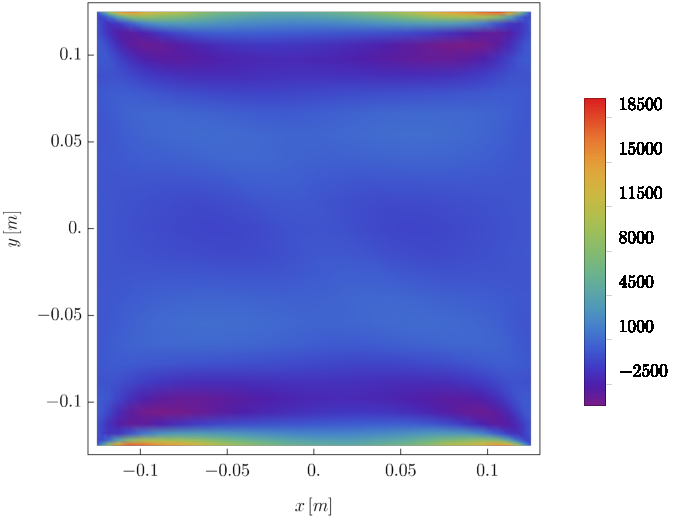
\includegraphics[width=.40\textwidth]{figures2/nxx6030.pdf}
		\label{fig:wdispa_cs1}
	}\hspace{0.1cm}
	\subfloat[][]
	{
		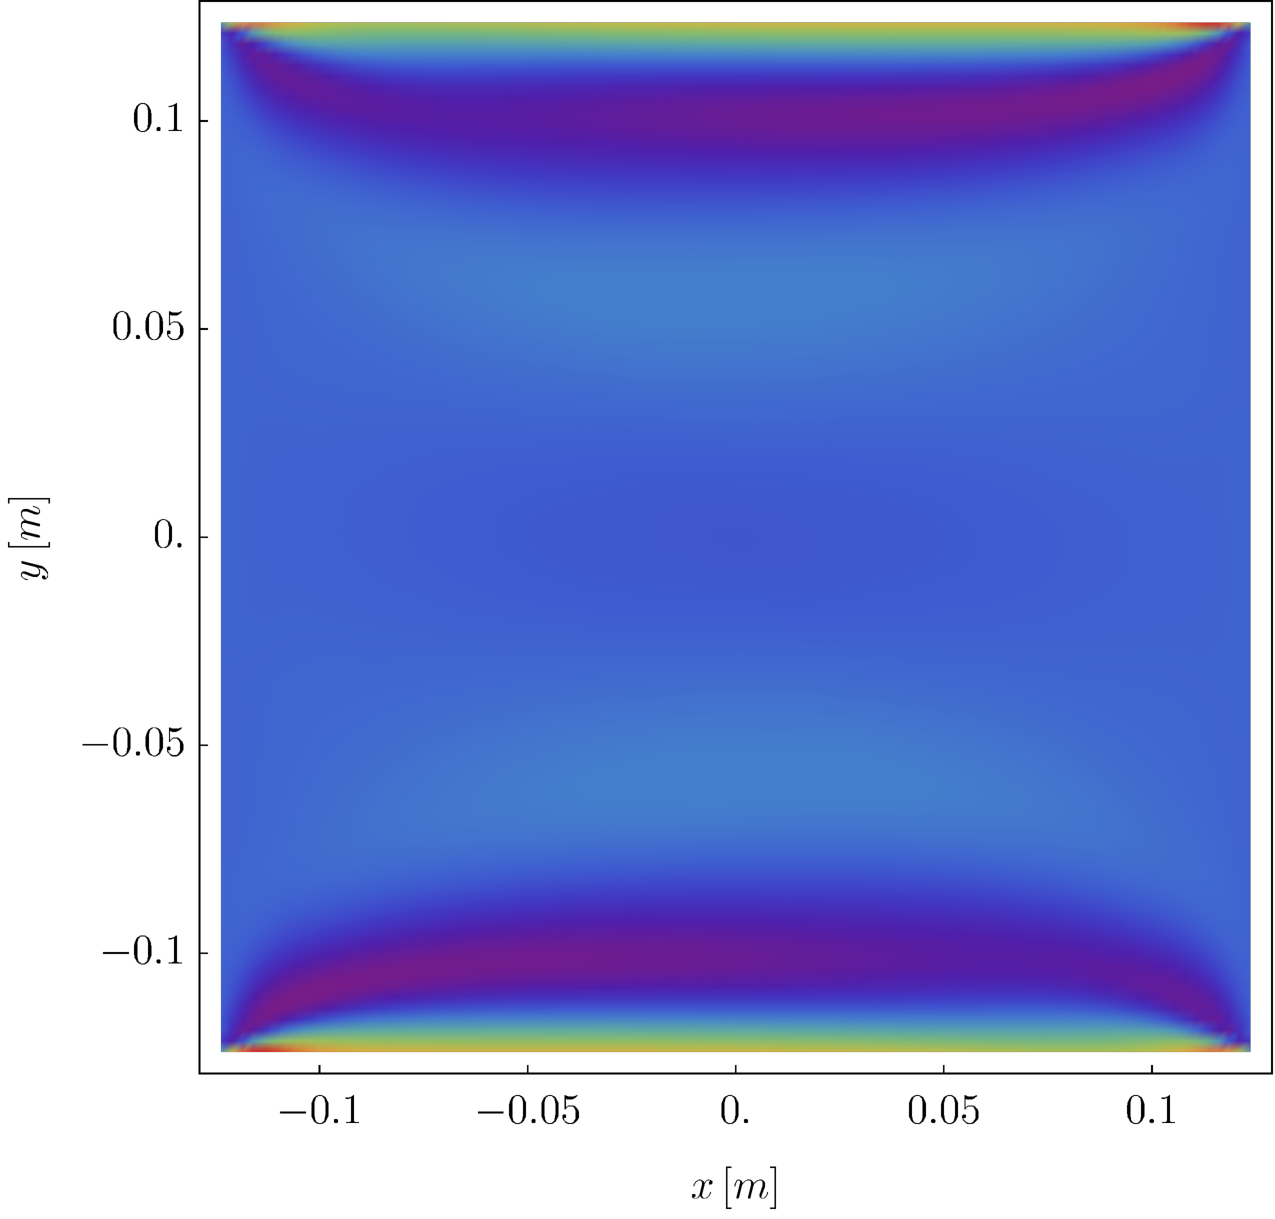
\includegraphics[width=.31\textwidth]{figures2/nxx6030fe.pdf}
		\label{fig:wdispb_cs1}
	}
	\\
	\subfloat[][]
	{
		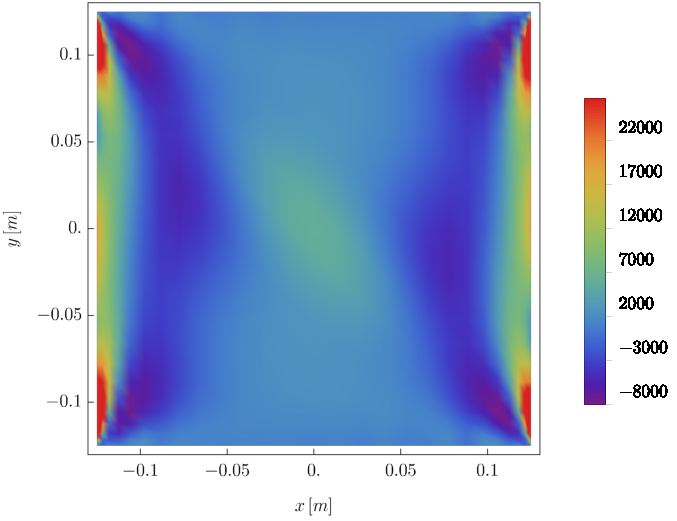
\includegraphics[width=.40\textwidth]{figures2/nyy6030clp.pdf}
		\label{fig:wdispc_cs1}
	}\hspace{0.2 cm}
	\subfloat[][]
	{
		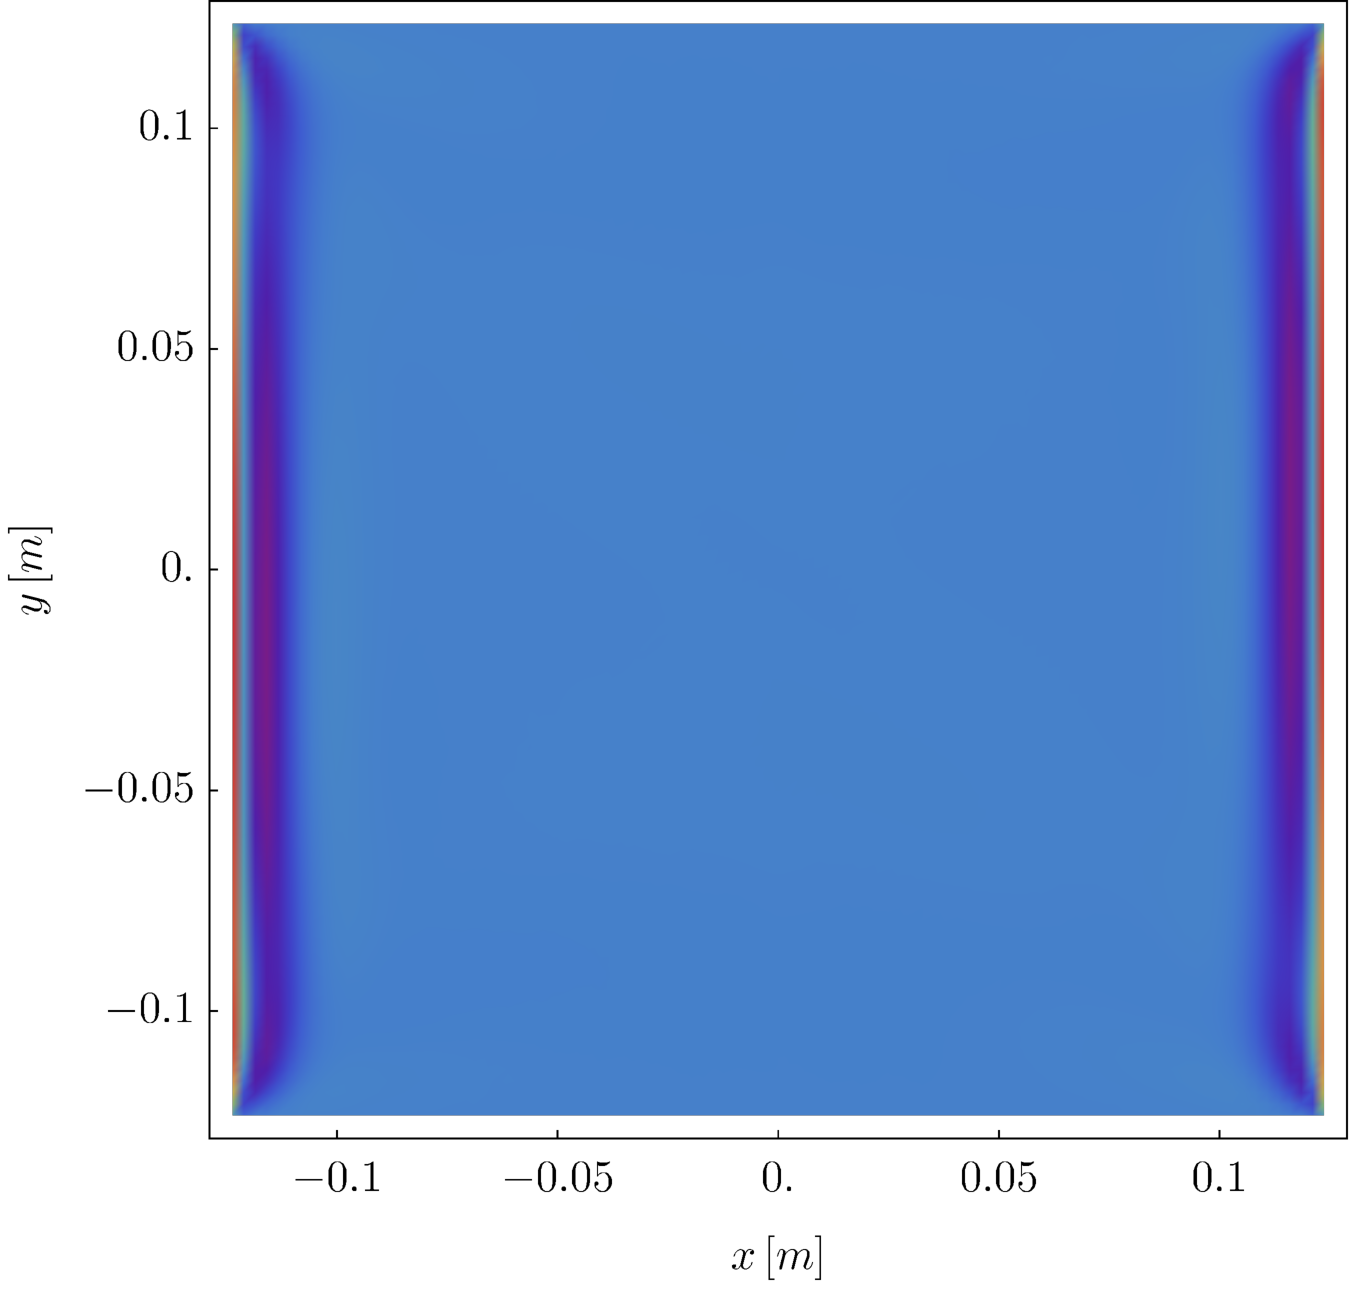
\includegraphics[width=.335\textwidth]{figures2/nyy6030feclp.pdf}
		\label{fig:wdispd_cs1}
	}
\\
	\subfloat[][]
	{
		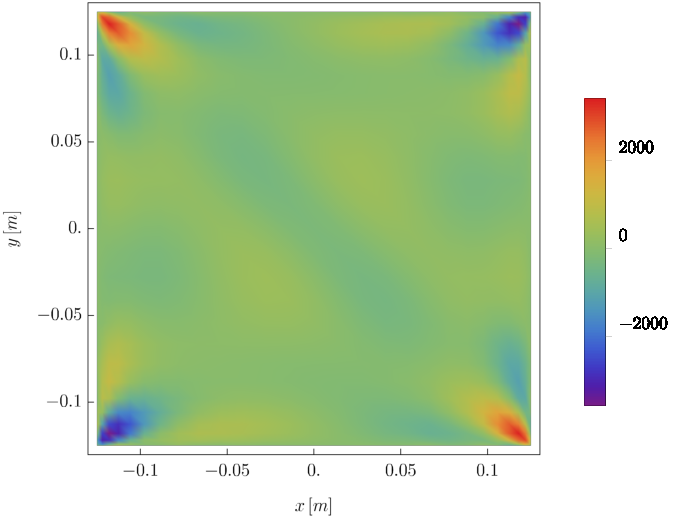
\includegraphics[width=.40\textwidth]{figures2/nxy6030.pdf}
		\label{fig:wdispa_cs1}
	}\hspace{0.2 cm}
	\subfloat[][]
	{
		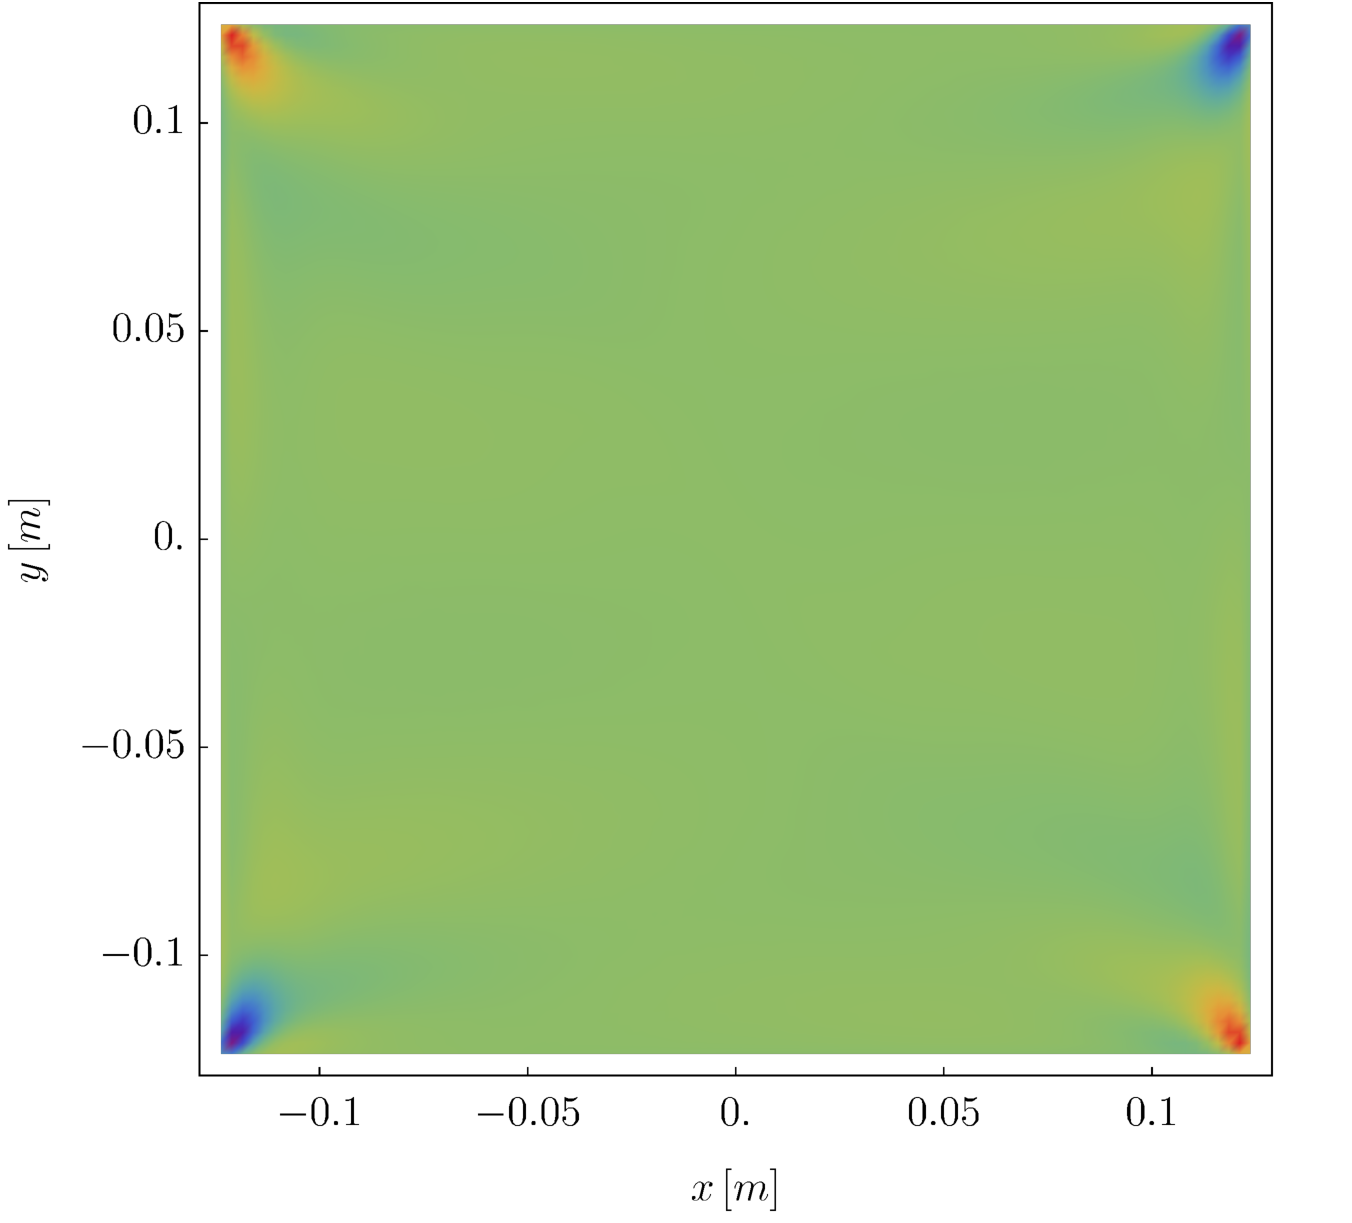
\includegraphics[width=.335\textwidth]{figures2/nxy6030fe.pdf}
		\label{fig:wdispb_cs1}
	}

	\caption{Investigated VS composites for $VS-3$ comparing the membrane stresses obtained from analytical method and FE: stress distribution $N_{xx}$ a) DDQM b) FE, stress distribution $N_{yy}$ a)DQM b) FE, stress distribution $N_{xy}$ a)DQM b) FE  }
	\label{fig:fiberpaths}
\end{figure}

\section{Parameteric Study}
phi= 0, one graph with change in t0 and t1, change in snapthrough and out-of-plane disp
\\
phi= 45, one graph with change in t0 and t1, change in snapthrough and out-of-plane disp

A geometrically nonlinear FE calculation was carried out in ABAQUS to simulate the snap-through process. The snap-through loads of several VS laminates described in Table \ref{data1} were calculated. The studied VS are depicted in Fig. \ref{fig:fiberpaths}. 

%$\Bigg \langle 3x+7 \bigg \rangle$

A certain family of VS laminates was chosen which satisfies, $\phi=0$ and $T_0+T_1=90$. Such laminates result in an average fiber orientation of  $[0_4/90_4]$, and therefore yields cylindrical shape with almost zero twisting curvature. In this paper, the snap-through loads and out-of-plane displacement is calculated from the developed analytical model and compared with FE results.  

The details of the VS laminate layup is given in Table \ref{data1}. All the investigated VS laminates yields cylindrical stable shape with almost zero twisting curvatures(Fig. \ref{fig:shapes}).  Fig. \ref{fig:rxn} shows the plot between the total reaction forces with the out-of-plane displacement. It can be observed that with the applied load, the structure deforms elastically featuring linear load-displacement curves. Once the critical point is detected, the structure snaps from one stable shape to another. It can be seen from the Fig. \ref{fig:rxn} that values of snap-through loads varies between different VS laminates. The value of snap forces are lower than $[0_4/90_4]$ cross-ply laminate for VS laminate satisfying $T_1>T_0$, whereas higher for VS laminates satisfying $T_1>T_0$. 
The snap-through force can be directly determined from the load-displacement curve. It can be observed from the figure that among all the laminates investigated, VS-4 requires the maximum snap-through force ($76.5$ N) followed by VS-3 ($71.0$ N), VS-1 ($25.7$ N) and VS-2 ($20.2$ N). The straight fiber cross-ply $[0_4/90_4]$ requires a snap-through force of $36.8$N, the value of whose are verified from the calculation carried out by Diaconu et al. \cite{Diaconu2009}. It can be observed that laminate VS-2 has $45\%$ lower snap-through forces than the straight cross-ply laminate, with a just $14\%$ lower out-of-plane displacement. It can be therefore observed that with VS laminate, there can be immense possibility to tailor the snap-through loads without much change in the shape of the bistable laminate. Such snap-through tailoring make VS laminates a promising option to be used in efficient morphing systems.
%\begin{table}[!htb]
%	\centering
%	\begin{tabular}{@{} l *5{d{2.6}} @{} } 
%		\hline
%		\mc{Laminate} & \mc{$[0_4/90_4]_\text{T}$}  &\mc{VS-1} &\mc{VS-2}  &\mc{VS-3} &\mc{VS-4}\\
%		\hline
%			\mc{FEM}   & 	\mc{36.8}  &  \mc{25.7} &   \mc{20.2} &  \mc{71.0} & \mc{76.4}\\
%		\hline
%	\end{tabular}
%	\vspace{5 mm}
%	\caption{Snap-through forces for plates with straight fibers and VS composites-in (N) }
%	\label{datasnap}
%\end{table}

%\begin{table}[!htb]
%	\centering
%	\setlength{\arrayrulewidth}{2\arrayrulewidth}
%	\begin{tabular}{lcccc}
%		\hline
%		{Type} & {$\phi$} & {$T_0$}  & {$T_1$} & {Layup}\\
%		\hline
%		{Straight} & {$45$}& {$\pm 45$} & {$\pm 45$} &{$\left[0_4/90_4\right]_\text{T}$}\\
%		{VS-1}  & {$45$}& {$\pm 15$} & {$\pm 75$} & {$[45\langle{15|75 \rangle}_4/45\langle {-15|-75 \rangle}_4]_\text{T}$}\\
%		{VS-2}  & {$45$}& {$\pm 30$} & {$\pm 60$} & {$[45\langle{30|60 \rangle}_4/45\langle {-30|-60 \rangle}_4]_\text{T}$}\\
%		{VS-3} & {$45$} & {$\pm 60$} & {$\pm 30$} & {$[45\langle{60|30 \rangle}_4/45\langle {-60|-30 \rangle}_4]_\text{T}$}\\ 
%		{VS-4} & {$45$} & {$\pm 75$} & {$\pm 15$} & {$[45\langle{75|15 \rangle}_4/45\langle {-75|-15 \rangle}_4]_\text{T}$}\\
%		\hline
%	\end{tabular}
%	\vspace{5 mm}
%	\caption{Fiber orientation and layup data for the investigated straight cross-ply and various VS composites}
%	\label{data1}
%\end{table}

\begin{figure}[!htb]
	\captionsetup[subfloat]{farskip=2pt,captionskip=2pt}
	\centering
	{
		\def\tkzscl{0.5}     
		% This file was created by matlab2tikz.
%
%The latest updates can be retrieved from
%  http://www.mathworks.com/matlabcentral/fileexchange/22022-matlab2tikz-matlab2tikz
%where you can also make suggestions and rate matlab2tikz.
%
\definecolor{mycolor1}{rgb}{0.0,0.0,0.6}%
\definecolor{mycolor2}{rgb}{0.25,0.37,1.0}%
\definecolor{mycolor3}{rgb}{0.4,0.7,1.0}%
\definecolor{mycolor4}{rgb}{0.8,0.9,1}%
\definecolor{mycolor5}{rgb}{0.80,0.0,0.0}%
%
\begin{tikzpicture}

\begin{axis}[%
width=4.521in,
height=3.566in,
at={(0.758in,0.481in)},
scale only axis,
xmin=-0.08,
xmax=0.08,
scaled x ticks = false,
x tick label style={/pgf/number format/fixed},
ymin=-4,
ymax=4,
axis background/.style={fill=white},
xmajorgrids,
ymajorgrids,
legend style={legend cell align=left, align=left, draw=white!15!black}
]
\addplot [color=mycolor1,line width=1.5pt]
  table[row sep=crcr]{%
-0.049128126	0\\
-0.046993611	0.1\\
-0.044870193	0.2\\
-0.042753722	0.3\\
-0.04063975	0.4\\
-0.038523299	0.5\\
-0.03639855	0.6\\
-0.034258368	0.7\\
-0.03209356	0.8\\
-0.029891588	0.9\\
-0.027634059	1\\
-0.025291025	1.1\\
-0.022804606	1.2\\
-0.020018792	1.3\\
-0.019864225	1.305\\
-0.019707311	1.31\\
-0.019547828	1.315\\
-0.019385513	1.32\\
-0.019220063	1.325\\
-0.019051114	1.33\\
-0.018878231	1.335\\
-0.018700885	1.34\\
-0.018518425	1.345\\
-0.018330026	1.35\\
-0.018134629	1.355\\
-0.017930832	1.36\\
-0.017716709	1.365\\
-0.0174895	1.37\\
-0.017244991	1.375\\
-0.016976168	1.38\\
-0.01666963	1.385\\
-0.016292392	1.39\\
-0.015663208	1.395\\
};
\addlegendentry{VS-1}

\addplot [color=mycolor1,line width=1.0pt,forget plot]
table[row sep=crcr]{%
-0.015663208	1.395\\
	0.06	1.395\\
};
\addplot [color=mycolor1,line width=1.5pt,forget plot]
table[row sep=crcr]{%
	0.015663208	-1.395\\
	0.016292392	-1.39\\
	0.01666963	-1.385\\
	0.016976168	-1.38\\
	0.017244991	-1.375\\
	0.0174895	-1.37\\
	0.017716709	-1.365\\
	0.017930832	-1.36\\
	0.018134629	-1.355\\
	0.018330026	-1.35\\
	0.018518425	-1.345\\
	0.018700885	-1.34\\
	0.018878231	-1.335\\
	0.019051114	-1.33\\
	0.019220063	-1.325\\
	0.019385513	-1.32\\
	0.019547828	-1.315\\
	0.019707311	-1.31\\
	0.019864225	-1.305\\
	0.020018792	-1.3\\
	0.022804606	-1.2\\
	0.025291025	-1.1\\
	0.027634059	-1\\
	0.029891588	-0.9\\
	0.03209356	-0.8\\
	0.034258368	-0.7\\
	0.03639855	-0.6\\
	0.038523299	-0.5\\
	0.04063975	-0.4\\
	0.042753722	-0.3\\
	0.044870193	-0.2\\
	0.046993611	-0.1\\
	0.049128126	0\\
};


\addplot [color=mycolor1,line width=1.0pt,forget plot]
table[row sep=crcr]{%
	0.015663208	-1.395\\
	-0.06	-1.395\\
};

\addplot [color=mycolor2,line width=1.5pt]
  table[row sep=crcr]{%
-0.063342355	0\\
-0.061702341	0.1\\
-0.060069862	0.2\\
-0.058444255	0.3\\
-0.056824856	0.4\\
-0.055210989	0.5\\
-0.053601961	0.6\\
-0.051997042	0.7\\
-0.050395458	0.8\\
-0.048796369	0.9\\
-0.04719885	1\\
-0.045601862	1.1\\
-0.044004224	1.2\\
-0.042404565	1.3\\
-0.040801275	1.4\\
-0.039192422	1.5\\
-0.037575663	1.6\\
-0.035948095	1.7\\
-0.034306068	1.8\\
-0.032644886	1.9\\
-0.030958383	2\\
-0.029238227	2.1\\
-0.027472802	2.2\\
-0.025645221	2.3\\
-0.023729569	2.4\\
-0.021682779	2.5\\
-0.019422489	2.6\\
-0.016717771	2.7\\
-0.016392882	2.71\\
-0.0160467	2.72\\
-0.015669723	2.73\\
-0.015241953	2.74\\
-0.01470282	2.75\\
};
\addlegendentry{VS-2}

\addplot [color=mycolor2,line width=1.0pt,forget plot]
table[row sep=crcr]{%
	-0.01470282	2.75\\
	0.06 2.75\\
};

\addplot [color=mycolor2,line width=1.5pt,forget plot]
table[row sep=crcr]{%
0.01470282	-2.75\\
0.015241953	-2.74\\
0.015669723	-2.73\\
0.0160467	-2.72\\
0.016392882	-2.71\\
0.016717771	-2.7\\
0.019422489	-2.6\\
0.021682779	-2.5\\
0.023729569	-2.4\\
0.025645221	-2.3\\
0.027472802	-2.2\\
0.029238227	-2.1\\
0.030958383	-2\\
0.032644886	-1.9\\
0.034306068	-1.8\\
0.035948095	-1.7\\
0.037575663	-1.6\\
0.039192422	-1.5\\
0.040801275	-1.4\\
0.042404565	-1.3\\
0.044004224	-1.2\\
0.045601862	-1.1\\
0.04719885	-1\\
0.048796369	-0.9\\
0.050395458	-0.8\\
0.051997042	-0.7\\
0.053601961	-0.6\\
0.055210989	-0.5\\
0.056824856	-0.4\\
0.058444255	-0.3\\
0.060069862	-0.2\\
0.061702341	-0.1\\
0.063342355	0\\
};

\addplot [color=mycolor2,line width=1.0pt,forget plot]
table[row sep=crcr]{%
	0.01470282	-2.75\\
	-0.06 -2.75\\
};

\addplot [color=mycolor3,line width=1.5pt]
  table[row sep=crcr]{%
0.01764601	-3.31\\
0.017968646	-3.3\\
0.019827584	-3.2\\
0.021243714	-3.1\\
0.022557431	-3\\
0.023832878	-2.9\\
0.025094757	-2.8\\
0.02635496	-2.7\\
0.02761986	-2.6\\
0.028893057	-2.5\\
0.030176624	-2.4\\
0.031471741	-2.3\\
0.032779049	-2.2\\
0.034098853	-2.1\\
0.03543125	-2\\
0.036776211	-1.9\\
0.03813363	-1.8\\
0.039503355	-1.7\\
0.040885216	-1.6\\
0.042279033	-1.5\\
0.043684628	-1.4\\
0.045101831	-1.3\\
0.046530481	-1.2\\
0.047970431	-1.1\\
0.049421549	-1\\
0.050883713	-0.9\\
0.05235682	-0.8\\
0.053840779	-0.7\\
0.055335511	-0.6\\
0.056840951	-0.5\\
0.058357047	-0.4\\
0.059883758	-0.3\\
0.061421054	-0.2\\
0.062968919	-0.1\\
0.064527342	0\\
};
\addlegendentry{VS-3}

\addplot [color=mycolor3,line width=1.0pt,forget plot]
table[row sep=crcr]{%
	0.01764601	-3.31\\
	-0.06 -3.31\\
};



\addplot [color=mycolor3,line width=1.5pt,forget plot]
table[row sep=crcr]{%
	-0.064527342	0\\
	-0.062968919	0.1\\
	-0.061421054	0.2\\
	-0.059883758	0.3\\
	-0.058357047	0.4\\
	-0.056840951	0.5\\
	-0.055335511	0.6\\
	-0.053840779	0.7\\
	-0.05235682	0.8\\
	-0.050883713	0.9\\
	-0.049421549	1\\
	-0.047970431	1.1\\
	-0.046530481	1.2\\
	-0.045101831	1.3\\
	-0.043684628	1.4\\
	-0.042279033	1.5\\
	-0.040885216	1.6\\
	-0.039503355	1.7\\
	-0.03813363	1.8\\
	-0.036776211	1.9\\
	-0.03543125	2\\
	-0.034098853	2.1\\
	-0.032779049	2.2\\
	-0.031471741	2.3\\
	-0.030176624	2.4\\
	-0.028893057	2.5\\
	-0.02761986	2.6\\
	-0.02635496	2.7\\
	-0.025094757	2.8\\
	-0.023832878	2.9\\
	-0.022557431	3\\
	-0.021243714	3.1\\
	-0.019827584	3.2\\
	-0.017968646	3.3\\
	-0.01764601	3.31\\
};

\addplot [color=mycolor3,line width=1.0pt,forget plot]
table[row sep=crcr]{%
	-0.01764601	3.31\\
	0.06 3.31\\
};


\addplot [color=mycolor4,line width=1.5pt]
table[row sep=crcr]{%
	-0.053211958	0\\
	-0.051213031	0.1\\
	-0.04924465	0.2\\
	-0.047307222	0.3\\
	-0.045401188	0.4\\
	-0.043527019	0.5\\
	-0.041685215	0.6\\
	-0.039876305	0.7\\
	-0.038100833	0.8\\
	-0.036359342	0.9\\
	-0.034652343	1\\
	-0.032980259	1.1\\
	-0.031343347	1.2\\
	-0.029741561	1.3\\
	-0.028174345	1.4\\
	-0.026640282	1.5\\
	-0.025136501	1.6\\
	-0.023657579	1.7\\
	-0.022193272	1.8\\
	-0.022046997	1.81\\
	-0.021900652	1.82\\
	-0.021754207	1.83\\
	-0.021607627	1.84\\
	-0.021460876	1.85\\
	-0.021313912	1.86\\
	-0.021166694	1.87\\
	-0.021019172	1.88\\
	-0.020871293	1.89\\
	-0.020722999	1.9\\
	-0.020574225	1.91\\
	-0.020424899	1.92\\
	-0.020274943	1.93\\
	-0.020124265	1.94\\
	-0.019972765	1.95\\
	-0.019820329	1.96\\
	-0.019666828	1.97\\
	-0.019512112	1.98\\
	-0.019356012	1.99\\
	-0.019198329	2\\
	-0.019038828	2.01\\
	-0.018877236	2.02\\
	-0.01871322	2.03\\
	-0.018546381	2.04\\
	-0.018376223	2.05\\
	-0.018202125	2.06\\
	-0.018023289	2.07\\
	-0.017838661	2.08\\
	-0.017646803	2.09\\
	-0.017445664	2.1\\
	-0.017232141	2.11\\
	-0.017001132	2.12\\
	-0.016743099	2.13\\
	-0.016435592	2.14\\
	-0.015979874	2.15\\	
};
\addlegendentry{VS-4}


\addplot [color=mycolor4,line width=1.0pt,forget plot]
table[row sep=crcr]{%
	-0.015979874	2.15\\	
	0.06 	2.15\\	
};


\addplot [color=mycolor5, mark options={solid, mycolor5},line width=1.5pt]
table[row sep=crcr]{%
	-0.064362196	0\\
	-0.063156645	0.1\\
	-0.061951628	0.2\\
	-0.060747126	0.3\\
	-0.059543117	0.4\\
	-0.058339577	0.5\\
	-0.057136479	0.6\\
	-0.055933793	0.7\\
	-0.054731487	0.8\\
	-0.05352952	0.9\\
	-0.052327849	1\\
	-0.051126418	1.1\\
	-0.049925167	1.2\\
	-0.048724019	1.3\\
	-0.047522885	1.4\\
	-0.046321657	1.5\\
	-0.045120203	1.6\\
	-0.043918365	1.7\\
	-0.042715948	1.8\\
	-0.041512711	1.9\\
	-0.040308356	2\\
	-0.039102514	2.1\\
	-0.037894717	2.2\\
	-0.036684375	2.3\\
	-0.035470732	2.4\\
	-0.034252806	2.5\\
	-0.033029311	2.6\\
	-0.031798527	2.7\\
	-0.030558109	2.8\\
	-0.029304781	2.9\\
	-0.028033814	3\\
	-0.026738087	3.1\\
	-0.025406237	3.2\\
	-0.024018531	3.3\\
	-0.024018531	3.3\\
	-0.023875464	3.31\\
	-0.023731431	3.32\\
	-0.02358637	3.33\\
	-0.023440216	3.34\\
	-0.023292898	3.35\\
	-0.023144336	3.36\\
	-0.022994443	3.37\\
	-0.022843123	3.38\\
	-0.022690266	3.39\\
	-0.022535754	3.4\\
	-0.022379449	3.41\\
	-0.022221201	3.42\\
	-0.022060834	3.43\\
	-0.02189815	3.44\\
	-0.021732921	3.45\\
	-0.02156488	3.46\\
	-0.021393716	3.47\\
	-0.02121906	3.48\\
	-0.021040469	3.49\\
	-0.020857408	3.5\\
	-0.020669212	3.51\\
	-0.020475047	3.52\\
	-0.020273839	3.53\\
	-0.020064164	3.54\\
	-0.019844071	3.55\\
	-0.019610757	3.56\\
	-0.019359936	3.57\\
	-0.019084451	3.58\\
	-0.018770546	3.59\\
	-0.018383881	3.6\\
	-0.017716941	3.61\\
};
\addlegendentry{Straight}


\addplot [color=mycolor5,line width=1.0pt,forget plot]
table[row sep=crcr]{%
	-0.017716941	3.61\\
	0.06 	3.61\\
};

% unstable straight
%\addplot [color=mycolor5, dashed, mark options={solid, mycolor5},line width=1.5pt]
%table[row sep=crcr]{%
%	%	0.0172994	-3.611\\	
%	%	0.0171603	-3.61\\
%	0.01663685965515374	-3.6\\
%	%	0.0166369	-3.6\\
%	%	0.001533748	-3.6\\
%	%	0.0152089	-3.5\\
%	%	0.001272871	-3.5\\
%	0.0152 -3.5\\
%	%0.014566318799223538 -3.4\\
%	%0.01411615644507253 -3.3\\
%	%0.013753534629127172 -3.2\\
%	%0.013432304055200146 -3.1\\
%	%0.01312131880354749 -3.0\\
%	%0.01278704839991392 -2.9\\
%	%0.012363114891154546 -2.8\\
%	%
%	%
%	%	0.0145153		-3.4\\
%	%	0.001083437	-3.4\\
%	%	0.000934746	-3.3\\
%	0.000813043	-3.2\\
%	0.000710795	-3.1\\
%	0.000623363	-3\\
%	0.000547659	-2.9\\
%	0.000481509	-2.8\\
%	0.000423316	-2.7\\
%	0.000371871	-2.6\\
%	0.000326227	-2.5\\
%	0.00028563	-2.4\\
%	0.000249469	-2.3\\
%	0.000217236	-2.2\\
%	0.000188507	-2.1\\
%	0.00016292	-2\\
%	0.000140163	-1.9\\
%	0.000119966	-1.8\\
%	0.000102089	-1.7\\
%	8.63217e-05	-1.6\\
%	7.2472e-05	-1.5\\
%	6.0367e-05	-1.4\\
%	4.9848e-05	-1.3\\
%	4.07683e-05	-1.2\\
%	3.2991e-05	-1.1\\
%	2.63874e-05	-1\\
%	2.08353e-05	-0.9\\
%	1.62177e-05	-0.8\\
%	1.24222e-05	-0.7\\
%	9.34e-06	-0.6\\
%	6.86e-06	-0.5\\
%	4.89e-06	-0.4\\
%	3.32e-06	-0.3\\
%	2.05e-06	-0.2\\
%	9.74e-07	-0.1\\
%	3.64e-16	0\\
%	3.64e-16	0\\
%	-9.74e-07	0.1\\
%	-2.05e-06	0.2\\
%	-3.32e-06	0.3\\
%	-4.89e-06	0.4\\
%	-6.86e-06	0.5\\
%	-9.34e-06	0.6\\
%	-1.24222e-05	0.7\\
%	-1.62177e-05	0.8\\
%	-2.08353e-05	0.9\\
%	-2.63874e-05	1\\
%	-3.2991e-05	1.1\\
%	-4.07683e-05	1.2\\
%	-4.9848e-05	1.3\\
%	-6.0367e-05	1.4\\
%	-7.2472e-05	1.5\\
%	-8.63217e-05	1.6\\
%	-0.000102089	1.7\\
%	-0.000119966	1.8\\
%	-0.000140163	1.9\\
%	-0.00016292	2\\
%	-0.000188507	2.1\\
%	-0.000217236	2.2\\
%	-0.000249469	2.3\\
%	%	-0.00028563	2.4\\
%	%	-0.000326227	2.5\\
%	%	-0.000371871	2.6\\
%	%	-0.000423316	2.7\\
%	%	-0.000481509	2.8\\
%	%	-0.000547659	2.9\\
%	%	-0.01312131880354749 3.0\\
%	%	-0.000623363	3\\
%	%	-0.000710795	3.1\\
%	-0.000813043	3.2\\
%	%	-0.000934746	3.3\\
%	%	-0.0145153		3.4\\
%	%	-0.001083437	3.4\\
%	%	-0.001272871	3.5\\
%	-0.0152089		3.5\\
%	-0.01663685965515374	3.6\\
%	%	-0.001533747	3.6\\
%	%	-0.0175427	3.6113\\
%	%	-0.001975539	3.7\\
%};

%% VS-3 unstable
%\addplot [color=mycolor3, dashed, mark options={solid, mycolor3},line width=1.5pt]
%  table[row sep=crcr]{%
%	-0.016572378	3.31\\
%	-0.016572378	3.31\\
%	-0.01635053	3.3\\
%	-0.016196824	3.29\\
%	-0.016075551	3.28\\
%	-0.015974182	3.27\\
%	-0.015886575	3.26\\
%	-0.015809182	3.25\\
%	-0.015739736	3.24\\
%	-0.015676688	3.23\\
%	-0.01561892	3.22\\
%	-0.015565601	3.21\\
%	-0.015516087	3.2\\
%	-0.015469874	3.19\\
%	-0.015426552	3.18\\
%	-0.015385789	3.17\\
%	-0.015347307	3.16\\
%	-0.015310872	3.15\\
%	-0.015276286	3.14\\
%	-0.015243379	3.13\\
%	-0.015212003	3.12\\
%	-0.01518203	3.11\\
%	-0.015153345	3.1\\
%	-0.01512585	3.09\\
%	-0.015099455	3.08\\
%	-0.015074081	3.07\\
%	-0.015049655	3.06\\
%	-0.015026115	3.05\\
%	-0.015003401	3.04\\
%	-0.01498146	3.03\\
%	-0.014960244	3.02\\
%	-0.014939709	3.01\\
%		-0.014919813	3\\
%	-0.01490052	2.99\\
%	-0.014881794	2.98\\
%	-0.014863604	2.97\\
%	-0.014845919	2.96\\
%	-0.014828713	2.95\\
%	-0.014811959	2.94\\
%	-0.014795633	2.93\\
%	-0.014779712	2.92\\
%	-0.014764175	2.91\\
%	-0.014749002	2.9\\
%	-0.014734174	2.89\\
%	-0.014719673	2.88\\
%	-0.014705482	2.87\\
%	-0.014691586	2.86\\
%	-0.014677969	2.85\\
%	-0.014664615	2.84\\
%	-0.014651512	2.83\\
%	-0.014625999	2.81\\
%	-0.014510078	2.71\\
%	-0.014405441	2.61\\
%	-0.014305034	2.51\\
%	-0.014201507	2.41\\
%	-0.014086437	2.31\\
%	-0.013948215	2.21\\
%	-0.013758089	2.11\\
%	-0.013428758	2.01\\
%	-0.013068		1.91\\
%	0	0\\
%	0.013068	-1.91\\
%	0.013428758	-2.01\\
%	0.013758089	-2.11\\
%	0.013948215	-2.21\\
%	0.014086437	-2.31\\
%	0.014201507	-2.41\\
%	0.014305034	-2.51\\
%	0.014405441	-2.61\\
%	0.014510078	-2.71\\
%	0.014625999	-2.81\\
%	0.014651512	-2.83\\
%	0.014664615	-2.84\\
%	0.014677969	-2.85\\
%	0.014691586	-2.86\\
%	0.014705482	-2.87\\
%	0.014719673	-2.88\\
%	0.014734174	-2.89\\
%	0.014749002	-2.9\\
%	0.014764175	-2.91\\
%	0.014779712	-2.92\\
%	0.014795633	-2.93\\
%	0.014811959	-2.94\\
%	0.014828713	-2.95\\
%	0.014845919	-2.96\\
%	0.014863604	-2.97\\
%	0.014881794	-2.98\\
%	0.01490052	-2.99\\
%	0.014919813	-3\\
%	0.014939709	-3.01\\
%	0.014960244	-3.02\\
%	0.01498146	-3.03\\
%	0.015003401	-3.04\\
%	0.015026115	-3.05\\
%	0.015049655	-3.06\\
%	0.015074081	-3.07\\
%	0.015099455	-3.08\\
%	0.01512585	-3.09\\
%	0.015153345	-3.1\\
%	0.01518203	-3.11\\
%	0.015212003	-3.12\\
%	0.015243379	-3.13\\
%	0.015276286	-3.14\\
%	0.015310872	-3.15\\
%	0.015347307	-3.16\\
%	0.015385789	-3.17\\
%	0.015426552	-3.18\\
%	0.015469874	-3.19\\
%	0.015516087	-3.2\\
%	0.015565601	-3.21\\
%	0.01561892	-3.22\\
%	0.015676688	-3.23\\
%	0.015739736	-3.24\\
%	0.015809182	-3.25\\
%	0.015886575	-3.26\\
%	0.015974182	-3.27\\
%	0.016075551	-3.28\\
%	0.016196824	-3.29\\
%	0.01635053	-3.3\\
%	0.016572378	-3.31\\
%	0.016572378	-3.31\\
%};
%
%\addplot [color=mycolor4, dashed, mark options={solid, mycolor5},line width=1.5pt]
% table[row sep=crcr]{%
%	-0.015381746	2.15\\
%	-0.013977808	2.05\\
%	-0.013486719	1.95\\
%	-0.013154379	1.85\\
%	-0.012893406	1.75\\
%	-0.01266977	1.65\\
%	-0.012464955	1.55\\
%	-0.012266086	1.45\\
%	-0.012061753	1.35\\
%	-0.011838887	1.25\\
%	-0.011576908	1.15\\
%	-0.011228547	1.05\\
%	-0.01050509	0.95\\
%	0	0\\
%	0.01050509	-0.95\\
%	0.011228547	-1.05\\
%	0.011576908	-1.15\\
%	0.011838887	-1.25\\
%	0.012061753	-1.35\\
%	0.012266086	-1.45\\
%	0.012464955	-1.55\\
%	0.01266977	-1.65\\
%	0.012893406	-1.75\\
%	0.013154379	-1.85\\
%	0.013486719	-1.95\\
%	0.013977808	-2.05\\
%	0.015381746	-2.15\\
%};
%
\addplot [color=mycolor5, mark options={solid, mycolor5},line width=1.5pt,forget plot]
table[row sep=crcr]{%
	0.017716941	-3.61\\
	0.018383881	-3.6\\
	0.018770546	-3.59\\
	0.019084451	-3.58\\
	0.019359936	-3.57\\
	0.019610757	-3.56\\
	0.019844071	-3.55\\
	0.020064164	-3.54\\
	0.020273839	-3.53\\
	0.020475047	-3.52\\
	0.020669212	-3.51\\
	0.020857408	-3.5\\
	0.021040469	-3.49\\
	0.02121906	-3.48\\
	0.021393716	-3.47\\
	0.02156488	-3.46\\
	0.021732921	-3.45\\
	0.02189815	-3.44\\
	0.022060834	-3.43\\
	0.022221201	-3.42\\
	0.022379449	-3.41\\
	0.022535754	-3.4\\
	0.022690266	-3.39\\
	0.022843123	-3.38\\
	0.022994443	-3.37\\
	0.023144336	-3.36\\
	0.023292898	-3.35\\
	0.023440216	-3.34\\
	0.02358637	-3.33\\
	0.023731431	-3.32\\
	0.023875464	-3.31\\
	0.024018531	-3.3\\
	0.024018531	-3.3\\
	0.025406237	-3.2\\
	0.026738087	-3.1\\
	0.028033814	-3\\
	0.029304781	-2.9\\
	0.030558109	-2.8\\
	0.031798527	-2.7\\
	0.033029311	-2.6\\
	0.034252806	-2.5\\
	0.035470732	-2.4\\
	0.036684375	-2.3\\
	0.037894717	-2.2\\
	0.039102514	-2.1\\
	0.040308356	-2\\
	0.041512711	-1.9\\
	0.042715948	-1.8\\
	0.043918365	-1.7\\
	0.045120203	-1.6\\
	0.046321657	-1.5\\
	0.047522885	-1.4\\
	0.048724019	-1.3\\
	0.049925167	-1.2\\
	0.051126418	-1.1\\
	0.052327849	-1\\
	0.05352952	-0.9\\
	0.054731487	-0.8\\
	0.055933793	-0.7\\
	0.057136479	-0.6\\
	0.058339577	-0.5\\
	0.059543117	-0.4\\
	0.060747126	-0.3\\
	0.061951628	-0.2\\
	0.063156645	-0.1\\
	0.064362196	0\\
};
\addplot [color=mycolor5,line width=1.0pt,forget plot]
table[row sep=crcr]{%
	0.017716941	-3.61\\
	-0.06  -3.61\\
};

%\addplot [color=mycolor5, dashed, mark options={solid, mycolor5},line width=1.5pt]
%table[row sep=crcr]{%
%-0.017219104	3.61\\
%-0.016655235	3.6\\
%-0.016371688	3.59\\
%-0.016160944	3.58\\
%-0.015988662	3.57\\
%-0.015841082	3.56\\
%-0.015711043	3.55\\
%-0.015594257	3.54\\
%-0.015487918	3.53\\
%-0.015390071	3.52\\
%-0.01529929	3.51\\
%-0.015214497	3.5\\
%-0.015134854	3.49\\
%-0.015059694	3.48\\
%-0.014988477	3.47\\
%-0.014920758	3.46\\
%-0.014856163	3.45\\
%-0.014794377	3.44\\
%-0.014735131	3.43\\
%-0.014678193	3.42\\
%-0.014623359	3.41\\
%-0.014570451	3.4\\
%-0.014519313	3.39\\
%-0.014469806	3.38\\
%-0.014421803	3.37\\
%-0.014375193	3.36\\
%-0.014329874	3.35\\
%-0.014285754	3.34\\
%-0.01424275	3.33\\
%-0.014200783	3.32\\
%-0.014159784	3.31\\
%-0.014119687	3.3\\
%-0.014080432	3.29\\
%-0.014041961	3.28\\
%-0.014004223	3.27\\
%-0.013967168	3.26\\
%-0.013930749	3.25\\
%-0.013894924	3.24\\
%-0.01385965	3.23\\
%-0.013824889	3.22\\
%-0.013790603	3.21\\
%-0.013756755	3.2\\
%-0.013723312	3.19\\
%-0.013690241	3.18\\
%-0.013657509	3.17\\
%-0.013625085	3.16\\
%-0.013592938	3.15\\
%-0.01356104	3.14\\
%-0.01352936	3.13\\
%-0.01349787	3.12\\
%-0.013466541	3.11\\
%-0.013435345	3.1\\
%-0.013404253	3.09\\
%-0.013373237	3.08\\
%-0.013342268	3.07\\
%-0.013311316	3.06\\
%-0.013280352	3.05\\
%-0.013249345	3.04\\
%-0.013218263	3.03\\
%-0.013187074	3.02\\
%-0.013155745	3.01\\
%-0.013124238	3\\
%-0.012789841	2.9\\
%-0.01236561	2.8\\
%0	0\\
%0.01236561	-2.8\\
%0.012789841	-2.9\\
%0.013124238	-3\\
%0.013155745	-3.01\\
%0.013187074	-3.02\\
%0.013218263	-3.03\\
%0.013249345	-3.04\\
%0.013280352	-3.05\\
%0.013311316	-3.06\\
%0.013342268	-3.07\\
%0.013373237	-3.08\\
%0.013404253	-3.09\\
%0.013435345	-3.1\\
%0.013466541	-3.11\\
%0.01349787	-3.12\\
%0.01352936	-3.13\\
%0.01356104	-3.14\\
%0.013592938	-3.15\\
%0.013625085	-3.16\\
%0.013657509	-3.17\\
%0.013690241	-3.18\\
%0.013723312	-3.19\\
%0.013756755	-3.2\\
%0.013790603	-3.21\\
%0.013824889	-3.22\\
%0.01385965	-3.23\\
%0.013894924	-3.24\\
%0.013930749	-3.25\\
%0.013967168	-3.26\\
%0.014004223	-3.27\\
%0.014041961	-3.28\\
%0.014080432	-3.29\\
%0.014119687	-3.3\\
%0.014159784	-3.31\\
%0.014200783	-3.32\\
%0.01424275	-3.33\\
%0.014285754	-3.34\\
%0.014329874	-3.35\\
%0.014375193	-3.36\\
%0.014421803	-3.37\\
%0.014469806	-3.38\\
%0.014519313	-3.39\\
%0.014570451	-3.4\\
%0.014623359	-3.41\\
%0.014678193	-3.42\\
%0.014735131	-3.43\\
%0.014794377	-3.44\\
%0.014856163	-3.45\\
%0.014920758	-3.46\\
%0.014988477	-3.47\\
%0.015059694	-3.48\\
%0.015134854	-3.49\\
%0.015214497	-3.5\\
%0.01529929	-3.51\\
%0.015390071	-3.52\\
%0.015487918	-3.53\\
%0.015594257	-3.54\\
%0.015711043	-3.55\\
%0.015841082	-3.56\\
%0.015988662	-3.57\\
%0.016160944	-3.58\\
%0.016371688	-3.59\\
%0.016655235	-3.6\\
%0.017219104	-3.61\\
%};
%

\end{axis}
\end{tikzpicture}%          
	}
	\caption{Reaction force-displacement diagram showing the intermediate unstable path}
	\label{fig:rxn}
\end{figure}

\begin{figure}[!htb]
	\captionsetup[subfloat]{farskip=2pt,captionskip=2pt}
	\centering
	{
		\def\tkzscl{0.5}     
		% This file was created by matlab2tikz.
%
%The latest updates can be retrieved from
%  http://www.mathworks.com/matlabcentral/fileexchange/22022-matlab2tikz-matlab2tikz
%where you can also make suggestions and rate matlab2tikz.
%
\definecolor{mycolor1}{rgb}{0.0,0.0,0.6}%
\definecolor{mycolor2}{rgb}{0.25,0.37,1.0}%
\definecolor{mycolor3}{rgb}{0.4,0.7,1.0}%
\definecolor{mycolor4}{rgb}{0.8,0.9,1}%
\definecolor{mycolor5}{rgb}{0.80,0.0,0.0}%
%
\begin{tikzpicture}[thick,scale=0.75, every node/.style={transform shape}]

\begin{axis}[%
width=4.521in,
height=3.566in,
at={(0.758in,0.481in)},
scale only axis,
xmin=-0.08,
xmax=0.08,
scaled x ticks = false,
x tick label style={/pgf/number format/fixed},
ymin=-6,
ymax=6,
axis background/.style={fill=white},
xmajorgrids,
xminorgrids,
ymajorgrids,
yminorgrids,
legend style={legend cell align=left, align=left, draw=white!15!black}
]
\addplot [color=mycolor1,line width=1.5pt]
table[row sep=crcr]{%
	-0.0581337	-4.356225e-10\\
	-0.058095368	0.00499925\\
	-0.0580570317	0.009993175\\
	-0.05799952	0.017473525\\
	-0.057913234	0.02867\\
	-0.057783767	0.045409\\
	-0.057589482	0.07038525\\
	-0.057297874	0.10752175\\
	-0.05686008	0.1623635\\
	-0.05620262	0.24220225\\
	-0.05521398	0.3642425\\
	-0.05372864	0.53778\\
	-0.05150057	0.784965\\
	-0.04819694	1.12647\\
	-0.043595	1.559415\\
	-0.0387814	1.9633975\\
	-0.0337576	2.33641\\
	-0.0285185	2.671075\\
	-0.0231991	2.973175\\
	-0.0179697	3.23265\\
	-0.012906	3.324625\\
	-0.00797510000000001	3.3028\\
	-0.0032213	3.33865\\
	0.00121839999999999	2.672875\\
	0.0019279	1.3230675\\
	0.0019175	1.1506175\\
	0.00188049999999999	0.9483\\
	0.0017452	0.5858075\\
	0.0012031	0.091299\\
	0.000961199999999995	0.0351325\\
	0.000609399999999996	0.02659825\\
	8.53999999999994e-05	0.04001125\\
	-0.000221100000000002	-0.01388795\\
	-0.0010012	-1.329465\\
	-0.000970800000000001	-1.6717825\\
	-0.000896100000000004	-1.9391225\\
	-0.0007396	-2.244155\\
	-0.000450900000000004	-2.564925\\
	4.35999999999978e-05	-2.86835\\
	0.000850399999999994	-3.116625\\
	0.0021263	-3.278725\\
	0.0041062	-3.341075\\
	0.00715129999999999	-3.315925\\
	0.0102799	-3.27955\\
	0.0135098	-3.300575\\
	0.0167373	-3.27705\\
	0.0200506	-3.1607\\
	0.0234845	-2.98495\\
	0.0269938	-2.79105\\
	0.0323419	-2.471865\\
	0.035279	-2.27441\\
	0.0396342	-1.94858\\
	0.0420243	-1.753285\\
	0.0456043	-1.4393925\\
	0.0512473	-0.8891025\\
	0.0571033	-0.229718\\
	0.0583883	-0.06318\\
	0.0596683	0.10390575\\
	0.0615863	0.3679725\\
	0.0645053	0.8054775\\
	0.0696003	1.700765\\
	0.0716943	2.1331975\\
	0.0737683	2.606325\\
	0.0771353	3.4963\\
	0.0804813	4.57535\\
	0.0837413	5.885425\\
};
\addlegendentry{FE}

\addplot [color=mycolor5, mark options={solid, mycolor5},line width=1.5pt]
table[row sep=crcr]{%
	-0.064362196	0\\
	-0.063156645	0.1\\
	-0.061951628	0.2\\
	-0.060747126	0.3\\
	-0.059543117	0.4\\
	-0.058339577	0.5\\
	-0.057136479	0.6\\
	-0.055933793	0.7\\
	-0.054731487	0.8\\
	-0.05352952	0.9\\
	-0.052327849	1\\
	-0.051126418	1.1\\
	-0.049925167	1.2\\
	-0.048724019	1.3\\
	-0.047522885	1.4\\
	-0.046321657	1.5\\
	-0.045120203	1.6\\
	-0.043918365	1.7\\
	-0.042715948	1.8\\
	-0.041512711	1.9\\
	-0.040308356	2\\
	-0.039102514	2.1\\
	-0.037894717	2.2\\
	-0.036684375	2.3\\
	-0.035470732	2.4\\
	-0.034252806	2.5\\
	-0.033029311	2.6\\
	-0.031798527	2.7\\
	-0.030558109	2.8\\
	-0.029304781	2.9\\
	-0.028033814	3\\
	-0.026738087	3.1\\
	-0.025406237	3.2\\
	-0.024018531	3.3\\
	-0.024018531	3.3\\
	-0.023875464	3.31\\
	-0.023731431	3.32\\
	-0.02358637	3.33\\
	-0.023440216	3.34\\
	-0.023292898	3.35\\
	-0.023144336	3.36\\
	-0.022994443	3.37\\
	-0.022843123	3.38\\
	-0.022690266	3.39\\
	-0.022535754	3.4\\
	-0.022379449	3.41\\
	-0.022221201	3.42\\
	-0.022060834	3.43\\
	-0.02189815	3.44\\
	-0.021732921	3.45\\
	-0.02156488	3.46\\
	-0.021393716	3.47\\
	-0.02121906	3.48\\
	-0.021040469	3.49\\
	-0.020857408	3.5\\
	-0.020669212	3.51\\
	-0.020475047	3.52\\
	-0.020273839	3.53\\
	-0.020064164	3.54\\
	-0.019844071	3.55\\
	-0.019610757	3.56\\
	-0.019359936	3.57\\
	-0.019084451	3.58\\
	-0.018770546	3.59\\
	-0.018383881	3.6\\
	-0.017716941	3.61\\
	-0.0175427		3.6113\\
};
\addlegendentry{Str}




\addplot [color=mycolor5, mark options={solid, mycolor5},line width=1.5pt]
table[row sep=crcr]{%
	0.0175427	-3.6113\\
	0.0176277	-3.611\\
	0.017716941	-3.61\\
	0.018383881	-3.6\\
	0.018770546	-3.59\\
	0.019084451	-3.58\\
	0.019359936	-3.57\\
	0.019610757	-3.56\\
	0.019844071	-3.55\\
	0.020064164	-3.54\\
	0.020273839	-3.53\\
	0.020475047	-3.52\\
	0.020669212	-3.51\\
	0.020857408	-3.5\\
	0.021040469	-3.49\\
	0.02121906	-3.48\\
	0.021393716	-3.47\\
	0.02156488	-3.46\\
	0.021732921	-3.45\\
	0.02189815	-3.44\\
	0.022060834	-3.43\\
	0.022221201	-3.42\\
	0.022379449	-3.41\\
	0.022535754	-3.4\\
	0.022690266	-3.39\\
	0.022843123	-3.38\\
	0.022994443	-3.37\\
	0.023144336	-3.36\\
	0.023292898	-3.35\\
	0.023440216	-3.34\\
	0.02358637	-3.33\\
	0.023731431	-3.32\\
	0.023875464	-3.31\\
	0.024018531	-3.3\\
	0.024018531	-3.3\\
	0.025406237	-3.2\\
	0.026738087	-3.1\\
	0.028033814	-3\\
	0.029304781	-2.9\\
	0.030558109	-2.8\\
	0.031798527	-2.7\\
	0.033029311	-2.6\\
	0.034252806	-2.5\\
	0.035470732	-2.4\\
	0.036684375	-2.3\\
	0.037894717	-2.2\\
	0.039102514	-2.1\\
	0.040308356	-2\\
	0.041512711	-1.9\\
	0.042715948	-1.8\\
	0.043918365	-1.7\\
	0.045120203	-1.6\\
	0.046321657	-1.5\\
	0.047522885	-1.4\\
	0.048724019	-1.3\\
	0.049925167	-1.2\\
	0.051126418	-1.1\\
	0.052327849	-1\\
	0.05352952	-0.9\\
	0.054731487	-0.8\\
	0.055933793	-0.7\\
	0.057136479	-0.6\\
	0.058339577	-0.5\\
	0.059543117	-0.4\\
	0.060747126	-0.3\\
	0.061951628	-0.2\\
	0.063156645	-0.1\\
	0.064362196	0\\
};

\addplot [color=mycolor5, dashed, mark options={solid, mycolor5},line width=1.5pt]
table[row sep=crcr]{%
%	0.0172994	-3.611\\	
%	0.0171603	-3.61\\
0.01663685965515374	-3.6\\
%	0.0166369	-3.6\\
%	0.001533748	-3.6\\
%	0.0152089	-3.5\\
%	0.001272871	-3.5\\
0.0152 -3.5\\
%0.014566318799223538 -3.4\\
%0.01411615644507253 -3.3\\
%0.013753534629127172 -3.2\\
%0.013432304055200146 -3.1\\
%0.01312131880354749 -3.0\\
%0.01278704839991392 -2.9\\
%0.012363114891154546 -2.8\\
%
%
%	0.0145153		-3.4\\
%	0.001083437	-3.4\\
%	0.000934746	-3.3\\
	0.000813043	-3.2\\
	0.000710795	-3.1\\
	0.000623363	-3\\
	0.000547659	-2.9\\
	0.000481509	-2.8\\
	0.000423316	-2.7\\
	0.000371871	-2.6\\
	0.000326227	-2.5\\
	0.00028563	-2.4\\
	0.000249469	-2.3\\
	0.000217236	-2.2\\
	0.000188507	-2.1\\
	0.00016292	-2\\
	0.000140163	-1.9\\
	0.000119966	-1.8\\
	0.000102089	-1.7\\
	8.63217e-05	-1.6\\
	7.2472e-05	-1.5\\
	6.0367e-05	-1.4\\
	4.9848e-05	-1.3\\
	4.07683e-05	-1.2\\
	3.2991e-05	-1.1\\
	2.63874e-05	-1\\
	2.08353e-05	-0.9\\
	1.62177e-05	-0.8\\
	1.24222e-05	-0.7\\
	9.34e-06	-0.6\\
	6.86e-06	-0.5\\
	4.89e-06	-0.4\\
	3.32e-06	-0.3\\
	2.05e-06	-0.2\\
	9.74e-07	-0.1\\
	3.64e-16	0\\
	3.64e-16	0\\
	-9.74e-07	0.1\\
	-2.05e-06	0.2\\
	-3.32e-06	0.3\\
	-4.89e-06	0.4\\
	-6.86e-06	0.5\\
	-9.34e-06	0.6\\
	-1.24222e-05	0.7\\
	-1.62177e-05	0.8\\
	-2.08353e-05	0.9\\
	-2.63874e-05	1\\
	-3.2991e-05	1.1\\
	-4.07683e-05	1.2\\
	-4.9848e-05	1.3\\
	-6.0367e-05	1.4\\
	-7.2472e-05	1.5\\
	-8.63217e-05	1.6\\
	-0.000102089	1.7\\
	-0.000119966	1.8\\
	-0.000140163	1.9\\
	-0.00016292	2\\
	-0.000188507	2.1\\
	-0.000217236	2.2\\
	-0.000249469	2.3\\
%	-0.00028563	2.4\\
%	-0.000326227	2.5\\
%	-0.000371871	2.6\\
%	-0.000423316	2.7\\
%	-0.000481509	2.8\\
%	-0.000547659	2.9\\
%	-0.01312131880354749 3.0\\
%	-0.000623363	3\\
%	-0.000710795	3.1\\
	-0.000813043	3.2\\
%	-0.000934746	3.3\\
%	-0.0145153		3.4\\
%	-0.001083437	3.4\\
%	-0.001272871	3.5\\
	-0.0152089		3.5\\
	-0.01663685965515374	3.6\\
%	-0.001533747	3.6\\
%	-0.0175427	3.6113\\
%	-0.001975539	3.7\\
};
%\addplot [color=mycolor5, dashed, mark options={solid, mycolor5},line width=1.5pt]
%table[row sep=crcr]{%
%-0.017219104	3.61\\
%-0.016655235	3.6\\
%-0.016371688	3.59\\
%-0.016160944	3.58\\
%-0.015988662	3.57\\
%-0.015841082	3.56\\
%-0.015711043	3.55\\
%-0.015594257	3.54\\
%-0.015487918	3.53\\
%-0.015390071	3.52\\
%-0.01529929	3.51\\
%-0.015214497	3.5\\
%-0.015134854	3.49\\
%-0.015059694	3.48\\
%-0.014988477	3.47\\
%-0.014920758	3.46\\
%-0.014856163	3.45\\
%-0.014794377	3.44\\
%-0.014735131	3.43\\
%-0.014678193	3.42\\
%-0.014623359	3.41\\
%-0.014570451	3.4\\
%-0.014519313	3.39\\
%-0.014469806	3.38\\
%-0.014421803	3.37\\
%-0.014375193	3.36\\
%-0.014329874	3.35\\
%-0.014285754	3.34\\
%-0.01424275	3.33\\
%-0.014200783	3.32\\
%-0.014159784	3.31\\
%-0.014119687	3.3\\
%-0.014080432	3.29\\
%-0.014041961	3.28\\
%-0.014004223	3.27\\
%-0.013967168	3.26\\
%-0.013930749	3.25\\
%-0.013894924	3.24\\
%-0.01385965	3.23\\
%-0.013824889	3.22\\
%-0.013790603	3.21\\
%-0.013756755	3.2\\
%-0.013723312	3.19\\
%-0.013690241	3.18\\
%-0.013657509	3.17\\
%-0.013625085	3.16\\
%-0.013592938	3.15\\
%-0.01356104	3.14\\
%-0.01352936	3.13\\
%-0.01349787	3.12\\
%-0.013466541	3.11\\
%-0.013435345	3.1\\
%-0.013404253	3.09\\
%-0.013373237	3.08\\
%-0.013342268	3.07\\
%-0.013311316	3.06\\
%-0.013280352	3.05\\
%-0.013249345	3.04\\
%-0.013218263	3.03\\
%-0.013187074	3.02\\
%-0.013155745	3.01\\
%-0.013124238	3\\
%-0.012789841	2.9\\
%-0.01236561	2.8\\
%0	0\\
%0.01236561	-2.8\\
%0.012789841	-2.9\\
%0.013124238	-3\\
%0.013155745	-3.01\\
%0.013187074	-3.02\\
%0.013218263	-3.03\\
%0.013249345	-3.04\\
%0.013280352	-3.05\\
%0.013311316	-3.06\\
%0.013342268	-3.07\\
%0.013373237	-3.08\\
%0.013404253	-3.09\\
%0.013435345	-3.1\\
%0.013466541	-3.11\\
%0.01349787	-3.12\\
%0.01352936	-3.13\\
%0.01356104	-3.14\\
%0.013592938	-3.15\\
%0.013625085	-3.16\\
%0.013657509	-3.17\\
%0.013690241	-3.18\\
%0.013723312	-3.19\\
%0.013756755	-3.2\\
%0.013790603	-3.21\\
%0.013824889	-3.22\\
%0.01385965	-3.23\\
%0.013894924	-3.24\\
%0.013930749	-3.25\\
%0.013967168	-3.26\\
%0.014004223	-3.27\\
%0.014041961	-3.28\\
%0.014080432	-3.29\\
%0.014119687	-3.3\\
%0.014159784	-3.31\\
%0.014200783	-3.32\\
%0.01424275	-3.33\\
%0.014285754	-3.34\\
%0.014329874	-3.35\\
%0.014375193	-3.36\\
%0.014421803	-3.37\\
%0.014469806	-3.38\\
%0.014519313	-3.39\\
%0.014570451	-3.4\\
%0.014623359	-3.41\\
%0.014678193	-3.42\\
%0.014735131	-3.43\\
%0.014794377	-3.44\\
%0.014856163	-3.45\\
%0.014920758	-3.46\\
%0.014988477	-3.47\\
%0.015059694	-3.48\\
%0.015134854	-3.49\\
%0.015214497	-3.5\\
%0.01529929	-3.51\\
%0.015390071	-3.52\\
%0.015487918	-3.53\\
%0.015594257	-3.54\\
%0.015711043	-3.55\\
%0.015841082	-3.56\\
%0.015988662	-3.57\\
%0.016160944	-3.58\\
%0.016371688	-3.59\\
%0.016655235	-3.6\\
%0.017219104	-3.61\\
%};



%\addplot [color=mycolor3, mark options={solid, mycolor5},line width=1.5pt]
%table[row sep=crcr]{%
%0.06510857424306747  0.  \\
%0.06422114553755351  -0.1  \\
%0.06333230026763914  -0.2  \\
%0.0624419425467815  -0.30000000000000004  \\
%0.061549969394468  -0.4  \\
%0.060656270178724526  -0.5  \\
%0.059760726014672444  -0.6000000000000001  \\
%0.05886320911616158  -0.7000000000000001  \\
%0.0579635820974739  -0.8  \\
%0.05706169722212092  -0.9  \\
%0.056157395595866855  -1.  \\
%0.05525050630133016  -1.1  \\
%0.054340845471885044  -1.2000000000000002  \\
%0.05342821530315098  -1.3  \\
%0.05251240300118554  -1.4000000000000001  \\
%0.0515931796676665  -1.5  \\
%0.050670299123965916  -1.6  \\
%0.04974349667822228  -1.7000000000000002  \\
%0.04881248784247595  -1.8  \\
%0.04787696701087638  -1.9000000000000001  \\
%0.046936606115180066  -2.  \\
%0.045991053280599874  -2.1  \\
%0.04503993151400047  -2.2  \\
%0.044082837468036665  -2.3000000000000003  \\
%0.04311934033981943  -2.4000000000000004  \\
%0.042148980981946034  -2.5  \\
%0.04117127132829902  -2.6  \\
%0.040185694268128354  -2.7  \\
%0.039191704140946554  -2.8000000000000003  \\
%0.03818872807308011  -2.9000000000000004  \\
%0.03717616843555312  -3.  \\
%0.0361534067729537  -3.1  \\
%0.03511980963337362  -3.2  \\
%0.03407473681719389  -3.3000000000000003  \\
%0.03301755264968537  -3.4000000000000004  \\
%0.03194764095375372  -3.5  \\
%0.030864424427091263  -3.6  \\
%0.02976738906609294  -3.7  \\
%0.02865611405318573  -3.8000000000000003  \\
%0.027530307022687724  -3.9000000000000004  \\
%0.02638984368212204  -4.  \\
%0.02523480917353004  -4.1000000000000005  \\
%0.02406553603766511  -4.2  \\
%0.022882629867192986  -4.3  \\
%0.021686968324444767  -4.4  \\
%0.020479651641669434  -4.5  \\
%0.019261872001643244  -4.6000000000000005  \\
%0.018034652599181494  -4.7  \\
%0.01679837682605239  -4.800000000000001  \\
%0.015551960772870547  -4.9  \\
%0.01429134736437232  -5.  \\
%0.013006475399439327  -5.1000000000000005  \\
%0.011673976452172668  -5.2  \\
%0.010233411529676384  -5.300000000000001  \\
%0.008437946596790284  -5.4  \\
%};
%\addlegendentry{$n=2$}

\end{axis}
\end{tikzpicture}%          
	}
	\caption{Reaction force-displacement diagram showing the intermediate unstable path}
	\label{fig:rxn}
\end{figure}


\begin{figure}[!h]
	\captionsetup[subfloat]{farskip=2pt,captionskip=2pt}
	\centering
	{
		\def\tkzscl{0.6}     
		% This file was created by matlab2tikz.
%
%The latest updates can be retrieved from
%  http://www.mathworks.com/matlabcentral/fileexchange/22022-matlab2tikz-matlab2tikz
%where you can also make suggestions and rate matlab2tikz.
%
\definecolor{mycolor1}{rgb}{0.0,0.0,0.6}%
\definecolor{mycolor2}{rgb}{0.25,0.37,1.0}%
\definecolor{mycolor3}{rgb}{0.4,0.7,1.0}%
\definecolor{mycolor4}{rgb}{0.8,0.9,1}%
\definecolor{mycolor5}{rgb}{0.80,0.0,0.0}%
%
\begin{tikzpicture}[thick,scale=0.75, every node/.style={transform shape}]

\begin{axis}[%
width=4.521in,
height=3.566in,
at={(0.758in,0.481in)},
%grid=both,
scale only axis,
xmin=-0.04,
xmax=0.14,
scaled x ticks = false,
x tick label style={/pgf/number format/fixed},
ymin=-20,
ymax=25,
axis background/.style={fill=white},
xmajorgrids,
ymajorgrids,
xtick distance=0.02,
ytick distance=5,
legend style={at={(0.785,0.857)}, anchor=south west, legend cell align=left, align=left, draw=white!15!black}
]
\addplot [color=mycolor5,line width=1.5pt]
  table[row sep=crcr]{%
0	-1.03717e-07\\
2.7502e-07	0.0019999\\
7.34151e-07	0.0039999\\
1.79154e-06	0.0069999\\
4.12315e-06	0.0114999\\
9.07837e-06	0.0182499\\
1.91972e-05	0.0283749\\
3.89185e-05	0.0435624\\
7.53428e-05	0.0663437\\
0.000138835	0.100516\\
0.000243625	0.151773\\
0.000409232	0.22866\\
0.000664054	0.34399\\
0.00105193	0.516985\\
0.00164116	0.776478\\
0.00254187	1.16572\\
0.00394167	1.74958\\
0.00608339	2.62536\\
0.00835175	3.50115\\
0.0107198	4.37694\\
0.0131961	5.25273\\
0.0157902	6.12851\\
0.0185209	7.0043\\
0.021428	7.88009\\
0.0245654	8.75588\\
0.0278802	9.63167\\
0.0311833	10.5075\\
0.0345253	11.3832\\
0.0382199	12.259\\
0.0391269	12.478\\
0.0398928	12.6969\\
0.0402277	12.779\\
0.0403702	12.8098\\
0.0404294	12.8214\\
0.0405332	12.8387\\
0.0405774	12.8452\\
0.0406649	12.8549\\
0.040705	12.8586\\
0.0407221	12.8599\\
0.0407547	12.862\\
0.0407685	12.8628\\
0.0407952	12.8639\\
0.0408064	12.8644\\
0.0408277	12.865\\
0.0408807	12.866\\
0.0409269	12.867\\
0.040969	12.8679\\
0.0410269	12.8694\\
0.0411056	12.8716\\
0.041213	12.8749\\
0.0413606	12.8798\\
0.0415615	12.8872\\
0.0418264	12.8983\\
0.0421634	12.915\\
0.0422849	12.9212\\
0.0423309	12.9236\\
0.0424008	12.9271\\
0.0424278	12.9284\\
0.0424715	12.9304\\
0.0424889	12.9311\\
0.0425197	12.9323\\
0.0431382	12.9339\\
0.0434996	12.9356\\
0.0437758	12.9373\\
0.0440197	12.9389\\
0.044356	12.9414\\
0.0448314	12.9452\\
0.0455122	12.9508\\
0.046489	12.9593\\
0.0478937	12.9719\\
0.0482421	12.9751\\
0.0485893	12.9783\\
0.0491116	12.983\\
0.0499218	12.9901\\
0.0502356	12.9928\\
0.0503555	12.9938\\
0.050547	12.9953\\
0.0506213	12.9959\\
0.0507506	12.9967\\
0.0507845	12.9969\\
0.0508207	12.9971\\
0.0508892	12.9975\\
0.0510783	12.9979\\
0.0513835	12.9984\\
0.0517638	12.9989\\
0.0521772	12.9994\\
0.0526005	12.9998\\
0.0532209	13.0006\\
0.0540929	13.0016\\
0.0552789	13.0032\\
0.0563756	13.0048\\
0.0574121	13.0064\\
0.0589003	13.0089\\
0.0603701	13.0113\\
0.0618611	13.0137\\
0.0634115	13.0161\\
0.0650629	13.0185\\
0.0668553	13.0209\\
0.0687814	13.0233\\
0.0707869	13.0257\\
0.0728161	13.0281\\
0.0748379	13.0305\\
0.0768417	13.0329\\
0.0788267	13.0353\\
0.0807973	13.0377\\
0.0827584	13.0402\\
0.0847233	13.0426\\
0.0852189	13.0432\\
0.0857167	13.0438\\
0.0864703	13.0447\\
0.0876407	13.046\\
0.0888452	13.0474\\
0.0900572	13.0487\\
0.0912584	13.0501\\
0.0930124	13.0521\\
0.0936621	13.0529\\
0.0946184	13.054\\
0.0960103	13.0557\\
0.0980018	13.0583\\
0.100775	13.0622\\
0.103337	13.066\\
0.105695	13.0699\\
0.107855	13.0737\\
0.108382	13.0747\\
0.108896	13.0757\\
0.109642	13.0771\\
0.110701	13.0793\\
0.112164	13.0825\\
0.112695	13.0837\\
0.113452	13.0856\\
0.114506	13.0883\\
0.115918	13.0924\\
0.117699	13.0986\\
0.119184	13.1048\\
0.120416	13.111\\
0.121431	13.1172\\
0.122579	13.1264\\
0.123725	13.1403\\
0.124482	13.1542\\
0.124981	13.1681\\
0.125406	13.189\\
0.125712	13.2202\\
0.125907	13.2672\\
0.126038	13.3375\\
0.126165	13.4431\\
0.126333	13.6014\\
0.126579	13.8389\\
0.126941	14.1951\\
0.127471	14.7295\\
0.12824	15.531\\
0.129338	16.7333\\
0.130867	18.5368\\
0.132047	20\\
0.132047	20\\
0.132016	19.98\\
0.132001	19.96\\
0.131978	19.93\\
0.131944	19.885\\
0.131892	19.8175\\
0.131815	19.7162\\
0.131698	19.5644\\
0.131521	19.3366\\
0.131252	18.9948\\
0.130839	18.4823\\
0.130203	17.7134\\
0.129203	16.5601\\
0.128813	16.1276\\
0.128212	15.4789\\
0.127273	14.5058\\
0.125776	13.0461\\
0.124159	11.5865\\
0.122413	10.1268\\
0.12052	8.6672\\
0.11847	7.20755\\
0.116246	5.7479\\
0.113831	4.28826\\
0.111212	2.82861\\
0.108372	1.36896\\
0.105497	0\\
0.105497	0\\
0.105497	-0.002\\
0.105496	-0.004\\
0.105495	-0.007\\
0.105493	-0.0115\\
0.105488	-0.01825\\
0.105478	-0.028375\\
0.105458	-0.0435625\\
0.105422	-0.0663437\\
0.105359	-0.100516\\
0.105255	-0.151773\\
0.105091	-0.22866\\
0.104839	-0.34399\\
0.104456	-0.516985\\
0.103873	-0.776478\\
0.102986	-1.16572\\
0.10159	-1.74958\\
0.0995003	-2.62536\\
0.0972929	-3.50115\\
0.0949956	-4.37694\\
0.0926087	-5.25273\\
0.0901326	-6.12851\\
0.0875623	-7.0043\\
0.0848819	-7.88009\\
0.0820535	-8.75588\\
0.0790252	-9.63167\\
0.0758302	-10.5075\\
0.07238	-11.3832\\
0.0682703	-12.259\\
0.063723	-13.1348\\
0.0646427	-13.5727\\
0.0638716	-14.0106\\
0.062913	-14.4485\\
0.0626149	-14.558\\
0.0624682	-14.599\\
0.0623989	-14.6144\\
0.0623661	-14.6202\\
0.062352	-14.6224\\
0.0623239	-14.6256\\
0.0623183	-14.6262\\
0.0623087	-14.6271\\
0.0622884	-14.6285\\
0.0622795	-14.629\\
0.0622588	-14.6298\\
0.0622493	-14.6301\\
0.062224	-14.6305\\
0.062212	-14.6307\\
0.0621704	-14.6309\\
0.0619842	-14.6312\\
0.0617831	-14.6313\\
0.0615812	-14.6315\\
0.061323	-14.6318\\
0.0610082	-14.6322\\
0.0606202	-14.6328\\
0.0601321	-14.6337\\
0.0595065	-14.6351\\
0.0586717	-14.6372\\
0.0574975	-14.6403\\
0.0557641	-14.645\\
0.0540174	-14.6497\\
0.0522286	-14.6544\\
0.0502988	-14.6591\\
0.0497976	-14.6603\\
0.0492508	-14.6614\\
0.049036	-14.6619\\
0.0486695	-14.6625\\
0.0485231	-14.6628\\
0.0482634	-14.6632\\
0.0476294	-14.6637\\
0.0469249	-14.6643\\
0.0462525	-14.6648\\
0.0456279	-14.6654\\
0.0447696	-14.6662\\
0.0435784	-14.6675\\
0.0424351	-14.6687\\
0.0413149	-14.67\\
0.0402009	-14.6712\\
0.0390816	-14.6725\\
0.0379494	-14.6737\\
0.0368046	-14.675\\
0.0356548	-14.6762\\
0.0345091	-14.6775\\
0.0340786	-14.6779\\
0.0334385	-14.6786\\
0.0324913	-14.6797\\
0.0310987	-14.6813\\
0.0290636	-14.6837\\
0.0270698	-14.686\\
0.0251116	-14.6884\\
0.0231828	-14.6908\\
0.0212729	-14.6932\\
0.0193613	-14.6955\\
0.0188768	-14.6961\\
0.0183887	-14.6967\\
0.0176502	-14.6976\\
0.0165107	-14.6989\\
0.016223	-14.6993\\
0.0159317	-14.6996\\
0.0154864	-14.7001\\
0.0148028	-14.7009\\
0.0137606	-14.702\\
0.0122003	-14.7037\\
0.00992693	-14.7062\\
0.00774651	-14.7088\\
0.00720848	-14.7094\\
0.00667674	-14.71\\
0.00589336	-14.711\\
0.00475101	-14.7124\\
0.00311155	-14.7145\\
0.00250821	-14.7154\\
0.00162651	-14.7166\\
0.000355931	-14.7184\\
-0.00143603	-14.7211\\
-0.00387688	-14.7251\\
-0.00607918	-14.7292\\
-0.00661324	-14.7302\\
-0.00713273	-14.7312\\
-0.00788031	-14.7327\\
-0.00893275	-14.735\\
-0.0103651	-14.7385\\
-0.0122161	-14.7436\\
-0.0137981	-14.7487\\
-0.0151422	-14.7539\\
-0.0162786	-14.759\\
-0.0176126	-14.7667\\
-0.0189989	-14.7783\\
-0.0199528	-14.7899\\
-0.0206075	-14.8015\\
-0.0210586	-14.813\\
-0.0214622	-14.8304\\
-0.0217665	-14.8564\\
-0.0219613	-14.8955\\
-0.0220836	-14.954\\
-0.0221881	-15.0419\\
-0.0223174	-15.1737\\
-0.0225033	-15.3714\\
-0.0227776	-15.6679\\
-0.0231817	-16.1127\\
-0.0237691	-16.7799\\
-0.0246156	-17.7807\\
-0.0258102	-19.2819\\
-0.0263523	-20\\
-0.0263523	-20\\
-0.0263522	-19.98\\
-0.0263373	-19.96\\
-0.0263151	-19.93\\
-0.0262816	-19.885\\
-0.0262312	-19.8175\\
-0.0261554	-19.7162\\
-0.026041	-19.5644\\
-0.0258679	-19.3366\\
-0.0256046	-18.9948\\
-0.0252011	-18.4823\\
-0.0245776	-17.7134\\
-0.0235968	-16.5601\\
-0.021972	-14.8301\\
-0.0213835	-14.1814\\
-0.0203963	-13.2083\\
-0.0187607	-11.7487\\
-0.0181899	-11.2013\\
-0.0172151	-10.3803\\
-0.0156123	-9.14868\\
-0.0150577	-8.68683\\
-0.0141138	-7.99407\\
-0.0125861	-6.95493\\
-0.0102207	-5.39622\\
-0.00758481	-3.8375\\
-0.00688577	-3.44782\\
-0.00617622	-3.05815\\
-0.00507695	-2.47363\\
-0.00465507	-2.25443\\
-0.00401214	-1.92564\\
-0.00302449	-1.43245\\
-0.00139342	-0.692675\\
-0.00111866	-0.519506\\
-0.000562814	-0.259753\\
4.83922e-06	0\\
};
\addlegendentry{stab}

\addplot [color=mycolor2]
  table[row sep=crcr]{%
0	-2.57249e-07\\
4.38428e-05	0.0195852\\
8.77171e-05	0.0394469\\
0.000153537	0.0692061\\
0.000252286	0.113759\\
0.000400451	0.180387\\
0.000622787	0.279848\\
0.000956485	0.427823\\
0.00145744	0.646512\\
0.00220969	0.965105\\
0.00334066	1.45491\\
0.00503914	2.15316\\
0.00758223	3.15249\\
0.0113118	4.53834\\
0.0159352	6.11434\\
0.0210093	7.6947\\
0.0265455	9.21848\\
0.0322936	10.7416\\
0.0379645	12.1145\\
0.0393592	12.5164\\
0.040795	12.8536\\
0.0438568	10.3742\\
0.0460297	10.4395\\
0.0481386	10.5073\\
0.0493053	10.4682\\
0.0499595	10.3323\\
0.0499911	10.3072\\
0.0500367	10.2647\\
0.0500565	10.2288\\
0.0500482	10.1202\\
0.0500216	10.0696\\
0.0499911	10.0253\\
0.0499421	9.96505\\
0.0498653	9.88141\\
0.0497474	9.76129\\
0.0495706	9.58033\\
0.0493338	9.31438\\
0.0489601	8.78982\\
0.0483664	7.47232\\
0.0481076	6.55533\\
0.0477509	4.08013\\
0.0477482	4.03185\\
0.0477458	3.98258\\
0.0477425	3.90718\\
0.0477382	3.79066\\
0.0477337	3.60833\\
0.0477325	3.31739\\
0.0477475	2.85138\\
0.0477948	2.31574\\
0.0478895	1.74925\\
0.0480547	1.16428\\
0.0483197	0.593215\\
0.0487266	0.0759961\\
0.0493338	-0.332294\\
0.0502213	-0.576376\\
0.0515041	-0.642249\\
0.0533532	-0.585334\\
0.0560069	-0.533755\\
0.0586234	-0.709303\\
0.0611866	-1.51451\\
0.061778	-2.03213\\
0.0622767	-2.81209\\
0.0626694	-3.67657\\
0.0630093	-4.49019\\
0.0633605	-5.22763\\
0.0637182	-5.98579\\
0.0639694	-6.96255\\
0.0639724	-7.2856\\
0.063919	-7.6734\\
0.0638395	-7.94258\\
0.0637957	-8.06451\\
0.063661	-8.35853\\
0.0636986	-8.28261\\
0.0637306	-8.21387\\
0.063761	-8.14487\\
0.0638028	-8.04159\\
0.0638554	-7.89254\\
0.0639109	-7.69381\\
0.0639615	-7.41443\\
0.0639733	-7.03311\\
0.0639325	-6.68184\\
0.0638547	-6.36715\\
0.0637012	-5.94413\\
0.0634323	-5.36937\\
0.0630224	-4.52065\\
0.06262	-3.56019\\
0.0621416	-2.56514\\
0.0615463	-1.79711\\
0.0608629	-1.3254\\
0.0601378	-1.03254\\
0.0593952	-0.84184\\
0.0582672	-0.664211\\
0.0565526	-0.544185\\
0.0539173	-0.562344\\
0.0511841	-0.640636\\
0.0482124	0.791743\\
0.048166	0.889695\\
0.0481199	0.995999\\
0.0480514	1.17493\\
0.0479506	1.49917\\
0.0478058	2.23222\\
0.0477454	2.89431\\
0.0477372	3.70303\\
0.0477459	3.97854\\
0.0477799	4.48574\\
0.0477668	4.32334\\
0.0477465	3.98954\\
0.047734	3.60417\\
0.0477761	2.50991\\
0.0478566	1.91526\\
0.0480045	1.31486\\
0.0482468	0.725022\\
0.0486223	0.183658\\
0.049186	-0.257328\\
0.0500129	-0.540194\\
0.0512097	-0.64011\\
0.052935	-0.599965\\
0.055415	-0.529145\\
0.0578564	-0.621993\\
0.0602676	-1.07622\\
0.0608608	-1.32525\\
0.0614323	-1.69805\\
0.061732	-1.99105\\
0.0618896	-2.18498\\
0.0621105	-2.51612\\
0.0624031	-3.07193\\
0.0627685	-3.9227\\
0.0631039	-4.698\\
0.0631927	-4.87979\\
0.0633236	-5.15871\\
0.0635268	-5.56838\\
0.0638121	-6.23812\\
0.0639749	-7.12209\\
0.0639578	-7.41805\\
0.0638928	-7.76173\\
0.0638235	-7.97851\\
0.0637855	-8.08047\\
0.0637047	-8.26405\\
0.0636623	-8.34996\\
0.063638	-8.3977\\
0.0635993	-8.46895\\
0.0638725	-7.83556\\
0.0638998	-7.73133\\
0.0639238	-7.62832\\
0.0639476	-7.48785\\
0.0639684	-7.28966\\
0.0639699	-7.01751\\
0.0639245	-6.65139\\
0.0637879	-6.17403\\
0.0636115	-5.74734\\
0.0634186	-5.34913\\
0.0631287	-4.75906\\
0.0627081	-3.77753\\
0.0622233	-2.71425\\
0.0616115	-1.86247\\
0.060896	-1.34289\\
0.060131	-1.0302\\
0.0593467	-0.831395\\
0.0581548	-0.650867\\
0.0563418	-0.536891\\
0.0535479	-0.573533\\
0.0506343	-0.618139\\
0.0498757	-0.510764\\
0.0490931	-0.2037\\
0.0478648	1.86049\\
0.0478495	1.95472\\
0.047834	2.04543\\
0.0478117	2.19117\\
0.0477812	2.43985\\
0.0477452	2.90355\\
0.047733	3.32509\\
0.0478107	4.80409\\
0.047866	5.25251\\
0.0479258	5.64443\\
0.0480189	6.14775\\
0.0481566	6.7494\\
0.0482397	7.05677\\
0.0483653	7.46354\\
0.0485544	7.97439\\
0.0486626	8.22226\\
0.0488259	8.5508\\
0.0490723	8.95928\\
0.0494581	9.45329\\
0.0496831	9.69121\\
0.0498035	9.81268\\
0.0498702	9.88121\\
0.0499699	9.9923\\
0.0500208	10.0621\\
0.0499622	9.98711\\
0.0498821	9.89366\\
0.0497979	9.80691\\
0.0496701	9.67777\\
0.049479	9.47631\\
0.0492202	9.16562\\
0.0487994	8.50088\\
0.0481638	6.77976\\
0.0480372	6.23517\\
0.0479677	5.88265\\
0.0478636	5.2357\\
0.0478115	4.8109\\
0.0477851	4.54305\\
0.0477503	4.05746\\
0.0477379	3.75926\\
0.0477365	3.13331\\
0.0477906	2.35664\\
0.0478967	1.71978\\
0.0480864	1.08167\\
0.048391	0.481588\\
0.0488569	-0.0366941\\
0.0495481	-0.416217\\
0.0505539	-0.610968\\
0.0520049	-0.630865\\
0.0540942	-0.553358\\
0.0561414	-0.533682\\
0.0581653	-0.651524\\
0.0601655	-1.04216\\
0.0620196	-2.37126\\
0.0623695	-3.00515\\
0.0626621	-3.66994\\
0.0629233	-4.30149\\
0.063185	-4.88204\\
0.0635974	-5.72341\\
0.0639375	-6.74467\\
0.0639698	-7.07784\\
0.0639493	-7.47603\\
0.0638909	-7.75183\\
0.0637245	-8.24963\\
0.063698	-8.27101\\
0.0636839	-8.30047\\
0.063662	-8.34453\\
0.0636279	-8.41024\\
0.0635729	-8.50772\\
0.0635439	-8.56205\\
0.0634941	-8.64159\\
0.0634485	-8.71779\\
0.0633626	-8.84854\\
0.0632179	-9.05397\\
0.063136	-9.16149\\
0.0629961	-9.33921\\
0.0627829	-9.59575\\
0.0624462	-9.97717\\
0.062121	-10.3333\\
0.0617958	-10.6865\\
0.0616143	-10.8863\\
0.0613433	-11.1924\\
0.0611961	-11.3641\\
0.060978	-11.6273\\
0.0608613	-11.7717\\
0.0606871	-11.9964\\
0.0604183	-12.3515\\
0.0600756	-12.7991\\
0.0598669	-13.0208\\
0.059686	-13.1289\\
0.0596308	-13.139\\
0.0595203	-13.116\\
0.059437	-13.06\\
0.0593612	-12.9809\\
0.059259	-12.8365\\
0.0591235	-12.5903\\
0.058942	-12.2046\\
0.0586863	-11.6412\\
0.058303	-10.9027\\
0.0581964	-10.7221\\
0.0580871	-10.5581\\
0.0579197	-10.3196\\
0.0576615	-9.99142\\
0.0575118	-9.81862\\
0.0572835	-9.57498\\
0.057016	-9.3142\\
0.0569271	-9.2318\\
0.0568377	-9.1515\\
0.0567014	-9.03296\\
0.0565355	-8.8933\\
0.0563296	-8.72711\\
0.0561216	-8.56548\\
0.0558379	-8.35316\\
0.0553685	-8.01416\\
0.0546289	-7.46683\\
0.0543014	-6.87202\\
0.0543404	-6.84811\\
0.0543136	-6.86141\\
0.054422	-6.79891\\
0.0545235	-6.76422\\
0.0546288	-6.73917\\
0.0547868	-6.71401\\
0.0548779	-6.70435\\
0.055015	-6.69422\\
0.055221	-6.68792\\
0.0553377	-6.68834\\
0.055513	-6.69363\\
0.0557758	-6.71009\\
0.0561671	-6.7547\\
0.0567628	-6.86877\\
0.0576587	-7.18712\\
0.0577063	-7.21147\\
0.057778	-7.25039\\
0.0578858	-7.31398\\
0.0580485	-7.42655\\
0.0582965	-7.64884\\
0.0587254	-8.44967\\
0.0588024	-8.81273\\
0.0588605	-9.18616\\
0.0589276	-9.51767\\
0.0589567	-9.61328\\
0.0589874	-9.69307\\
0.0590349	-9.78765\\
0.0591069	-9.88926\\
0.0592138	-9.98967\\
0.0593706	-10.0871\\
0.0595876	-10.1876\\
0.0599153	-10.3234\\
0.0604214	-10.4171\\
0.0604499	-10.4074\\
0.0604929	-10.3851\\
0.0605163	-10.3671\\
0.0605566	-10.3136\\
0.0605668	-10.285\\
0.0605709	-10.2446\\
0.0605611	-10.1981\\
0.0605296	-10.1473\\
0.0604647	-10.0979\\
0.0603478	-10.06\\
0.0601489	-10.0483\\
0.0598176	-10.0428\\
0.0596292	-9.80661\\
0.0597686	-9.05531\\
0.0598854	-8.39338\\
0.0599032	-8.22349\\
0.0599218	-7.95467\\
0.0599288	-7.50547\\
0.0599194	-7.23176\\
0.059884	-6.77577\\
0.0595846	-5.33388\\
0.059371	-4.83165\\
0.0591442	-4.51047\\
0.0588256	-4.2852\\
0.0583955	-4.20453\\
0.057821	-4.2592\\
0.0575075	-4.31503\\
0.0570543	-4.39894\\
0.0563983	-4.50334\\
0.0554445	-4.59814\\
0.05404	-4.6329\\
0.0519338	-4.53808\\
0.049825	-4.12995\\
0.0478496	-0.172784\\
0.0478295	0.0394145\\
0.0478103	0.26473\\
0.0477837	0.628891\\
0.0477495	1.24867\\
0.0477148	2.37042\\
0.0477248	4.72057\\
0.0479609	9.03537\\
0.0480462	10.4899\\
0.0480146	11.3727\\
0.047923	11.9202\\
0.047874	12.1677\\
0.0478875	12.6038\\
0.0479795	12.7516\\
0.0481651	12.8139\\
0.0483851	12.7999\\
0.0485711	12.7251\\
0.0488471	12.4899\\
0.0491968	11.9236\\
0.0496097	10.467\\
0.0497101	9.95263\\
0.0498137	9.37899\\
0.0498732	9.02944\\
0.0499648	8.46685\\
0.0500167	8.12985\\
0.050095	7.59751\\
0.0501853	6.92759\\
0.0502479	6.44443\\
0.0502811	6.17362\\
0.050329	5.78513\\
0.0503552	5.57954\\
0.050394	5.30121\\
0.0504502	4.97525\\
0.0505215	4.69621\\
0.0505915	4.53632\\
0.0506314	4.47601\\
0.0506928	4.41537\\
0.0507872	4.37617\\
0.0509308	4.40115\\
0.0511456	4.57198\\
0.0514677	5.10399\\
0.0516224	5.54633\\
0.051781	6.48377\\
0.0517988	6.85014\\
0.0517776	7.50435\\
0.0517709	7.59251\\
0.0517625	7.68211\\
0.0517476	7.82047\\
0.0517185	8.04595\\
0.0516511	8.45283\\
0.0515558	8.90104\\
0.0514057	9.47165\\
0.0511561	10.197\\
0.0508824	10.8343\\
0.0506091	11.3461\\
0.0502056	11.9196\\
0.0495891	12.4628\\
0.0489841	12.6694\\
0.0488412	12.6826\\
0.0486977	12.6806\\
0.048483	12.6573\\
0.0481624	12.5862\\
0.0476813	12.4154\\
0.0468914	11.9686\\
0.0468772	11.9576\\
0.0468625	11.946\\
0.0468403	11.928\\
0.0468065	11.8998\\
0.0467542	11.8542\\
0.0466719	11.7768\\
0.0465354	11.6336\\
0.0464513	11.5329\\
0.0464016	11.4681\\
0.0461081	10.7194\\
0.0461209	10.6932\\
0.0461368	10.6728\\
0.0461666	10.6554\\
0.046219	10.6453\\
0.0463108	10.659\\
0.0464686	10.7219\\
0.0467366	10.8672\\
0.0471834	11.0746\\
0.0479188	10.9118\\
0.0486102	8.2627\\
0.0493836	-5.3617\\
0.0501388	-6.09794\\
0.0509036	-6.51197\\
0.0520632	-6.90421\\
0.0538255	-7.30252\\
0.0565123	-7.7972\\
0.0592955	-8.34578\\
0.0622146	-9.11465\\
0.0629825	-9.39549\\
0.0637835	-9.77678\\
0.06426	-10.0957\\
0.0645463	-10.374\\
0.0647195	-10.6437\\
0.0648006	-10.9182\\
0.0647881	-11.2346\\
0.0646989	-11.5071\\
0.0645278	-11.8107\\
0.0642425	-12.1785\\
0.0637904	-12.6496\\
0.0630965	-13.2884\\
0.0627063	-13.6425\\
0.062132	-14.2074\\
0.0621047	-14.2418\\
0.0620652	-14.2967\\
0.062016	-14.3994\\
0.0620144	-14.4085\\
0.0620134	-14.4239\\
0.0620207	-14.4532\\
0.0620433	-14.4752\\
0.0620742	-14.4865\\
0.0621183	-14.491\\
0.0621822	-14.4869\\
0.0622755	-14.47\\
0.0624124	-14.4321\\
0.0626141	-14.3612\\
0.0629122	-14.2386\\
0.0633539	-14.0377\\
0.0640081	-13.7139\\
0.0649803	-13.2441\\
0.0664285	-12.6163\\
0.0686052	-11.9071\\
0.0719498	-11.2419\\
0.0754606	-10.3545\\
0.0790431	-9.36861\\
0.0825703	-8.32994\\
0.0878059	-6.63707\\
0.093008	-4.81309\\
0.0982584	-2.81986\\
0.103628	-0.574676\\
0.10922	2.06793\\
0.115242	5.43057\\
0.116425	6.17062\\
0.117603	6.93919\\
0.119371	8.15707\\
0.122089	10.2052\\
0.127132	14.749\\
0.129044	16.7713\\
0.13093	18.9999\\
0.133991	23.1917\\
};
\addlegendentry{riks}

\end{axis}
\end{tikzpicture}%          
	}
	\caption{Reaction force-displacement diagram showing the intermediate unstable path for $3060$}
	\label{fig:rxn}
\end{figure}

\begin{figure}[!h]
	\captionsetup[subfloat]{farskip=2pt,captionskip=2pt}
	\centering
	{
%		\def\tkzscl{0.3}     
		% This file was created by matlab2tikz.
%
%The latest updates can be retrieved from
%  http://www.mathworks.com/matlabcentral/fileexchange/22022-matlab2tikz-matlab2tikz
%where you can also make suggestions and rate matlab2tikz.
%
\definecolor{mycolor1}{rgb}{0.0,0.0,0.6}%
\definecolor{mycolor2}{rgb}{0.25,0.37,1.0}%
\definecolor{mycolor3}{rgb}{0.4,0.7,1.0}%
\definecolor{mycolor4}{rgb}{0.8,0.9,1}%
\definecolor{mycolor5}{rgb}{0.80,0.0,0.0}%
%
\begin{tikzpicture}[thick,scale=0.75, every node/.style={transform shape}]
\begin{axis}[%
width=4.521in,
height=3.566in,
at={(0.758in,0.481in)},
scale only axis,
xmin=-0.06,
xmax=0.06,
scaled x ticks = false,
x tick label style={/pgf/number format/fixed},
ymin=-2.5,
ymax=2.5,
axis background/.style={fill=white},
xmajorgrids,
xminorgrids,
ymajorgrids,
yminorgrids,
xtick distance=0.02,
legend style={legend cell align=left, align=left, draw=white!15!black}
]
\addplot [color=mycolor1,line width=1.5pt]
  table[row sep=crcr]{%
-0.050195051		0\\
-0.048738958		0.1\\
-0.047298489		0.2\\
-0.045868858		0.3\\
-0.044445269		0.4\\
-0.043022801		0.5\\
-0.041596272		0.6\\
-0.040160084		0.7\\
-0.038708012		0.8\\
-0.037232926		0.9\\
-0.0357264			1\\
-0.034178124		1.1\\
-0.032574999		1.2\\
-0.030899628		1.3\\
-0.029127644		1.4\\
-0.027222519		1.5\\
-0.025124141		1.6\\
-0.022718562		1.7\\
-0.019727004		1.8\\
-0.014668373		1.9\\
-0.01347594			1.91\\
};
\addlegendentry{n=3}

\addplot [color=mycolor2,dashed, line width=1.5pt]
table[row sep=crcr]{%
	-0.01347594			1.91\\
	-0.009321122	1.9\\
	-0.009429901	1.8\\
	-0.009529931	1.7\\
	-0.009617468	1.6\\
	-0.009686808	1.5\\
	-0.009728686	1.4\\
	-0.009726397	1.3\\
	-0.009643795	1.2\\
	-0.009364779	1.1\\
};



\addplot [color=mycolor2,dashed,line width=1.5pt]
table[row sep=crcr]{%
	-0.004732313	0\\
	-0.004880751	0.1\\
	-0.00502821		0.2\\
	-0.005173814	0.3\\
	-0.005316539	0.4\\
	-0.005455233	0.5\\
	-0.005588668	0.6\\
	-0.005715616	0.7\\
	-0.005834884	0.8\\
	-0.005945167	0.9\\
	-0.006045323	1\\
		-0.009364779	1.1\\
%	-0.006134723	1.1\\
%	-0.006213008	1.2\\
%	-0.006280014	1.3\\
%	-0.006335798	1.4\\
%	-0.006380609	1.5\\
%	-0.006414848	1.6\\
%	-0.006439021	1.7\\
%	-0.006453696	1.8\\
%	-0.006459468	1.9\\
};

\addplot [color=mycolor2,dashed,line width=1.5pt]
table[row sep=crcr]{%
	-0.004732313	0\\
	-0.004583618	-0.1\\
	-0.004435243	-0.2\\
	-0.00428763	-0.3\\
	-0.00414111	-0.4\\
	-0.003995914	-0.5\\
	-0.003852194	-0.6\\
	-0.003710036	-0.7\\
	-0.003569474	-0.8\\
	-0.003430501	-0.9\\
	-0.003293074	-1\\
	0.00936471	-1.1\\
%	-0.003157125	-1.1\\
%	-0.003022561	-1.2\\
%	-0.002889275	-1.3\\
%	-0.002757141	-1.4\\
%	-0.002626019	-1.5\\
%	-0.002495757	-1.6\\
%	-0.002366187	-1.7\\
%	-0.00223713	-1.8\\
%	-0.002108385	-1.9\\
};

\addplot [color=mycolor2,dashed,line width=1.5pt]
table[row sep=crcr]{%
	0.0135168	-1.91\\
	0.009321055	-1.9\\
	0.009429833	-1.8\\
	0.009529864	-1.7\\
	0.0096174	-1.6\\
	0.00968674	-1.5\\
	0.009728618	-1.4\\
	0.009726328	-1.3\\
	0.009643726	-1.2\\
	0.00936471	-1.1\\
};


\addplot [color=mycolor1,line width=1.5pt]
table[row sep=crcr]{%
0.050195155	0\\
0.048739047	-0.1\\
0.047298569	-0.2\\
0.045868934	-0.3\\
0.044445347	-0.4\\
0.043022887	-0.5\\
0.041596375	-0.6\\
0.040160213	-0.7\\
0.038708178	-0.8\\
0.037233143	-0.9\\
0.035726685	-1\\
0.034178502	-1.1\\
0.032575501	-1.2\\
0.030900299	-1.3\\
0.029128552	-1.4\\
0.027223773	-1.5\\
0.02512594	-1.6\\
0.022721326	-1.7\\
0.019732002	-1.8\\
0.014689927	-1.9\\
0.0135168	-1.91\\
};


\end{axis}
\node[inner sep=0pt] (ss1) at (3.3,5.2)
{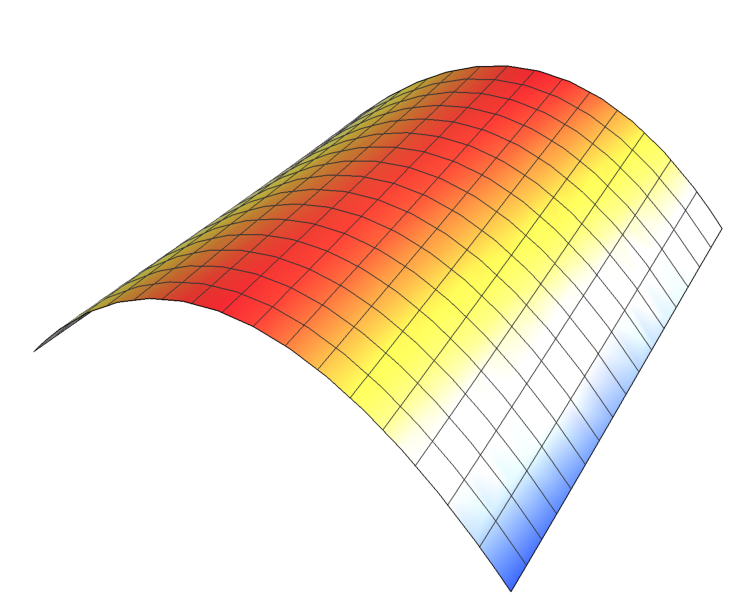
\includegraphics[width=.15\textwidth]{figures2/ss-1_f0.pdf}};

\node[inner sep=0pt] (ss1) at (5.7,9.9)
{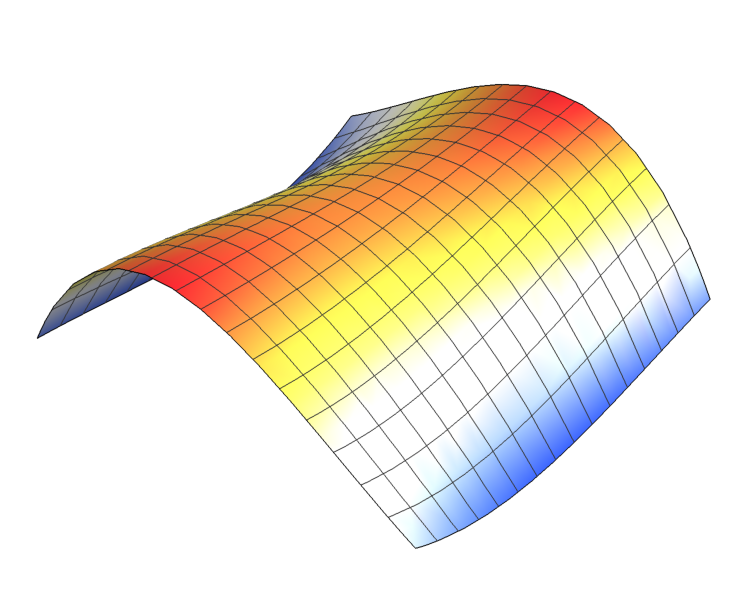
\includegraphics[width=.15\textwidth]{figures2/ss-1_f1,91.pdf}};

\node[inner sep=0pt] (ss1) at (7.658,8.3)
{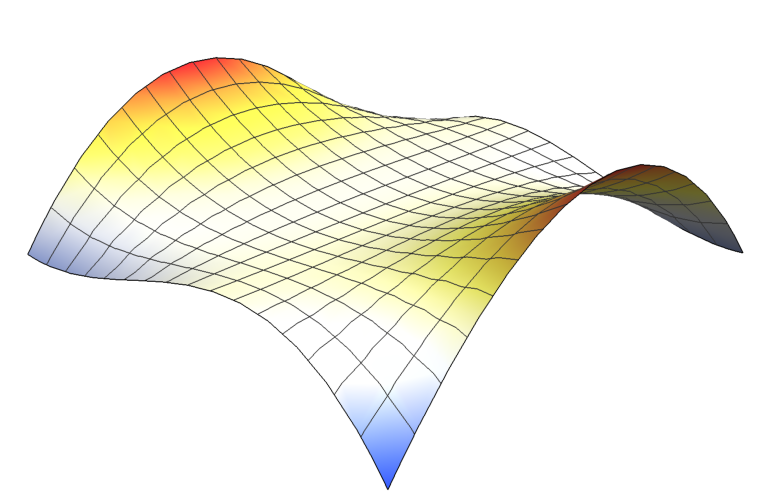
\includegraphics[width=.15\textwidth]{figures2/us-1_f1,6.pdf}};

\node[inner sep=0pt] (ss1) at (8.34,5)
{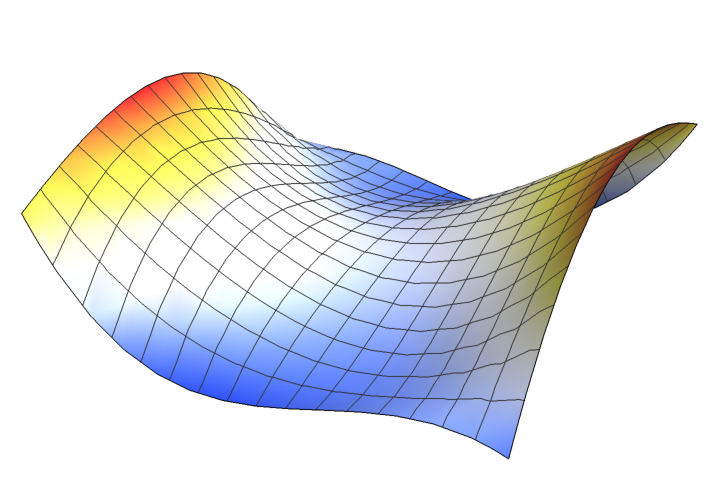
\includegraphics[width=.15\textwidth]{figures2/us-1_f0.pdf}};

\node[inner sep=0pt] (ss1) at (9.25,1.7)
{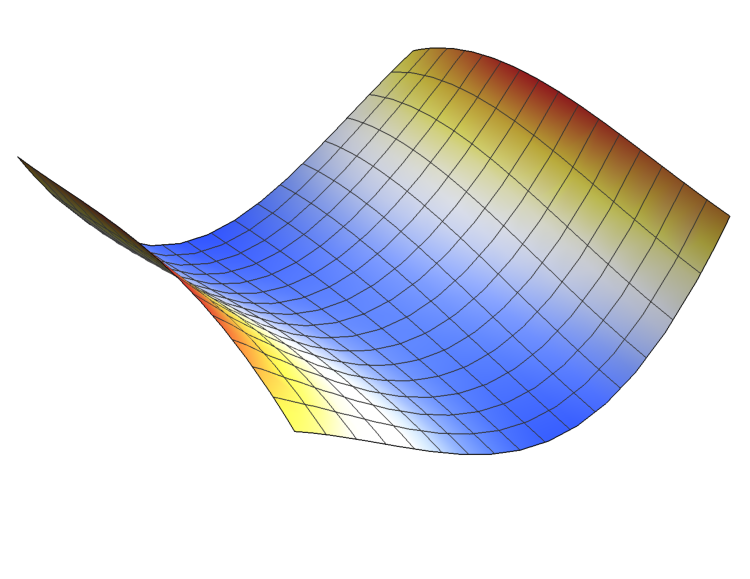
\includegraphics[width=.13\textwidth]{figures2/ss-2_f1,91.pdf}};

\node[inner sep=0pt] (ss1) at (11.66,5.8)
{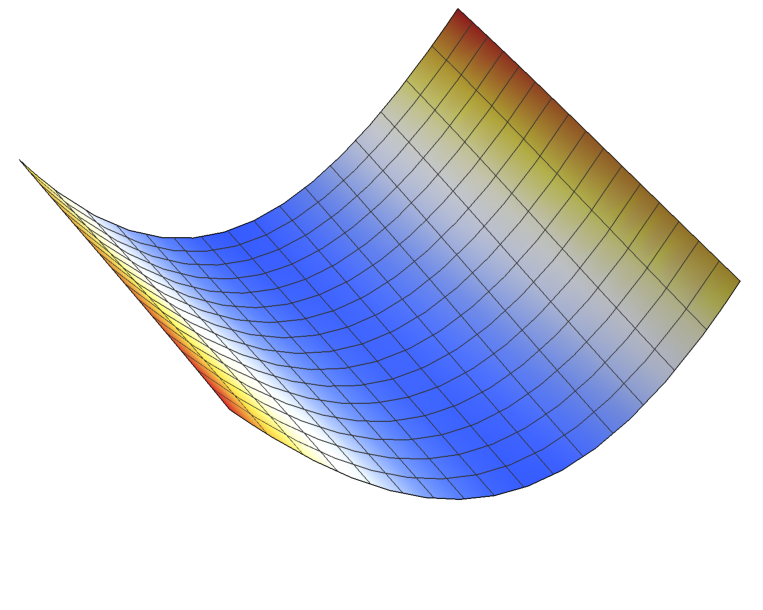
\includegraphics[width=.13\textwidth]{figures2/ss-2_f0.pdf}};

\end{tikzpicture}%




          
	}
	\caption{Analytical force-displacement diagram showing the intermediate unstable path for $1575$}
	\label{fig:rxn}
\end{figure}

%\begin{figure}[!htb]
%	\captionsetup[subfloat]{farskip=2pt,captionskip=2pt}
%	\centering
%	{
%		\def\tkzscl{0.6}     
%		% This file was created by matlab2tikz.
%
%The latest updates can be retrieved from
%  http://www.mathworks.com/matlabcentral/fileexchange/22022-matlab2tikz-matlab2tikz
%where you can also make suggestions and rate matlab2tikz.
%
\definecolor{mycolor1}{rgb}{0.63158,0.63158,0.63158}%
\definecolor{mycolor2}{rgb}{0.42105,0.42105,0.42105}%
\definecolor{mycolor3}{rgb}{0.36842,0.36842,0.36842}%
\definecolor{mycolor4}{rgb}{0.26316,0.26316,0.26316}%

\begin{tikzpicture}[scale=\tkzscl]

\begin{axis}[%
width=5.151in,
height=4.432in,
at={(0.864in,0.598in)},
scale only axis,
xmin=0,
xmax=0.06,
xlabel style={font=\color{white!15!black},font=\large},
xlabel={Displacement [m]},
ymin=-80,
ymax=100,
ylabel style={font=\color{white!15!black},font=\large},
ylabel={Reaction Force [N]},
axis background/.style={fill=white},
axis x line*=bottom,
axis y line*=left,
xmajorgrids,
ymajorgrids,
legend style={at={(0.95,0.32)}, font=\large,legend cell align=left, align=left, fill=none, draw=none},
ticklabel style={font=\large}
]
\addplot [color=blue,dashdotted,line width=1.0pt,mark=otimes*,mark size=2.0,mark options={solid}] table[row sep=crcr]{%
x	y\\
0	-6.99446e-06\\
6.81502e-07	0.00184354\\
1.6847e-06	0.00517202\\
3.49345e-06	0.0116077\\
6.43132e-06	0.0223308\\
1.09626e-05	0.039016\\
1.78103e-05	0.0642802\\
2.80975e-05	0.102243\\
4.35348e-05	0.159201\\
6.66991e-05	0.24464\\
0.000101464	0.372799\\
0.000153651	0.565037\\
0.000232025	0.853394\\
0.000349796	1.28593\\
0.00052693	1.93475\\
0.000793733	2.90804\\
0.00119651	4.36816\\
0.00180679	6.5592\\
0.00273743	9.84912\\
0.00417551	14.7686\\
0.00570321	19.769\\
0.00733746	24.7689\\
0.00916504	29.7666\\
0.0115376	34.7684\\
0.0124044	36.0114\\
0.012895	36.4785\\
0.0131388	36.6527\\
0.0137865	36.9027\\
0.0139125	36.9004\\
0.0139735	36.8925\\
0.0141312	36.8553\\
0.0142082	36.8225\\
0.0144271	36.6899\\
0.0145399	36.5865\\
0.0145876	36.5375\\
0.0146757	36.4353\\
0.0148822	36.1349\\
0.0149757	35.9691\\
0.0151823	35.5147\\
0.0152736	35.2789\\
0.0154614	34.6855\\
0.0155421	34.3964\\
0.0156967	33.744\\
0.016209	30.5342\\
0.0164912	28.3448\\
0.0177034	17.2896\\
0.0182715	11.9993\\
0.0194207	0.603747\\
0.0226968	-37.7893\\
0.0252465	-49.0726\\
0.0274514	-49.8699\\
0.0294332	-45.6797\\
0.032019	-36.16\\
0.0351642	-22.3081\\
0.0442791	20.7449\\
0.046292	32.5703\\
0.0467796	35.8409\\
0.0469023	36.7039\\
0.0469372	36.9535\\
0.0469444	37.0045\\
0.0469456	37.0125\\
0.046946	37.0145\\
0.0469464	37.0166\\
0.0469471	37.0196\\
0.0469482	37.0241\\
0.0469498	37.0309\\
0.0469521	37.0411\\
0.0469557	37.0563\\
0.046961	37.0792\\
0.046969	37.1135\\
0.046981	37.165\\
0.046999	37.2423\\
0.047026	37.3581\\
0.0470665	37.5319\\
0.0471271	37.7926\\
0.0472179	38.1836\\
0.0473538	38.7701\\
0.0475571	39.6498\\
0.0478607	40.9695\\
0.048313	42.9487\\
0.0489845	45.9164\\
0.049894	49.9926\\
0.049894	49.9926\\
0.0497835	49.5055\\
};
\addlegendentry{Straight[$0_4/90_4]$}

\addplot [color=mycolor1,dashdotted,line width=1.0pt,mark=square,mark size=2.5,mark options={solid}] table[row sep=crcr]{%
x	y\\
0	1.32649e-07\\
7.76736e-07	0.00118105\\
1.98807e-06	0.00361635\\
4.34903e-06	0.00894351\\
8.45629e-06	0.0186836\\
1.5082e-05	0.0347366\\
2.53118e-05	0.0597109\\
4.07942e-05	0.0975803\\
6.40739e-05	0.154517\\
9.90325e-05	0.239953\\
0.000151538	0.368112\\
0.000230445	0.560352\\
0.000349145	0.848714\\
0.000527965	1.28127\\
0.000797962	1.9302\\
0.00120705	2.90404\\
0.00183029	4.36726\\
0.00278825	6.57569\\
0.00428443	9.83725\\
0.00668922	14.7639\\
0.00942811	19.7644\\
0.0131105	24.7628\\
0.0134891	25.0676\\
0.0143481	25.5272\\
0.0144788	25.5541\\
0.0146186	25.5687\\
0.0146812	25.5694\\
0.0148146	25.5569\\
0.0148739	25.5451\\
0.0150008	25.5038\\
0.0150567	25.479\\
0.0151716	25.4115\\
0.0152209	25.3764\\
0.0153157	25.2951\\
0.0155852	24.9635\\
0.0157274	24.71\\
0.0157886	24.5863\\
0.0159077	24.3013\\
0.0159575	24.171\\
0.0160467	23.908\\
0.0162568	23.1137\\
0.0163545	22.683\\
0.0166206	21.0954\\
0.0167532	20.1751\\
0.0168101	19.7568\\
0.0169189	18.868\\
0.0170211	17.9526\\
0.0180409	0.813453\\
0.0189049	-8.58274\\
0.0195762	-13.5376\\
0.0201233	-16.3748\\
0.0207751	-18.1511\\
0.0215616	-18.4158\\
0.0225507	-16.9874\\
0.0287433	-0.274407\\
0.0342054	19.6148\\
0.0355763	25.203\\
0.0356901	25.6346\\
0.0356952	25.71\\
0.035696	25.7123\\
0.0356964	25.7138\\
0.0356971	25.7158\\
0.0356981	25.7188\\
0.0356996	25.7233\\
0.0357018	25.7301\\
0.0357052	25.7403\\
0.0357102	25.7555\\
0.0357178	25.7784\\
0.0357292	25.8127\\
0.0357462	25.8642\\
0.0357717	25.9414\\
0.03581	26.0573\\
0.0358674	26.2311\\
0.0359533	26.4917\\
0.036082	26.8827\\
0.0362744	27.4692\\
0.0365619	28.3488\\
0.0369905	29.6677\\
0.0376276	31.6436\\
0.0385708	34.5959\\
0.0399561	39.0719\\
0.0414753	44.0741\\
0.0429563	49.0749\\
0.0432279	49.9979\\
0.0432279	49.9979\\
};
\addlegendentry{VS-1}

\addplot [color=mycolor2,solid,line width=1.0pt,mark=triangle,mark size=2.5,mark options={solid}]table[row sep=crcr]{%
x	y\\
0	-1.33392e-06\\
5.52787e-07	0.000944614\\
1.39964e-06	0.00285252\\
3.00538e-06	0.0068733\\
5.72543e-06	0.0139853\\
1.00294e-05	0.0254358\\
1.66063e-05	0.0430273\\
2.65213e-05	0.069575\\
4.14137e-05	0.109441\\
6.37709e-05	0.169247\\
9.73438e-05	0.258958\\
0.000147786	0.393525\\
0.000223639	0.595375\\
0.000337851	0.89815\\
0.000510169	1.35232\\
0.000770982	2.03359\\
0.00116779	3.05561\\
0.00177683	4.58923\\
0.00272797	6.88727\\
0.00426488	10.3357\\
0.00603751	13.8347\\
0.0082853	17.335\\
0.00901052	18.2077\\
0.0104997	19.518\\
0.0114135	20.0016\\
0.0122553	20.1616\\
0.0127946	19.9378\\
0.0129219	19.8992\\
0.0130847	19.8177\\
0.0135131	19.5206\\
0.013725	19.3109\\
0.0142984	18.5948\\
0.0145899	18.0777\\
0.0155987	15.4767\\
0.0162443	12.7897\\
0.0165715	11.0043\\
0.0167094	10.1457\\
0.0169765	8.10366\\
0.0170879	7.1594\\
0.0172979	5.014\\
0.0173839	4.05088\\
0.017539	1.99642\\
0.0179696	-8.48305\\
0.0184686	-16.8011\\
0.0189507	-21.1586\\
0.019593	-24.3099\\
0.0204268	-26.2663\\
0.0215119	-26.6481\\
0.0229484	-25.1884\\
0.0283554	-17.4636\\
0.033969	2.64296\\
0.0368409	16.3719\\
0.0375053	19.8072\\
0.0375826	20.1985\\
0.0375893	20.2534\\
0.0375902	20.257\\
0.0375911	20.2601\\
0.0375925	20.2645\\
0.0375946	20.2712\\
0.0375977	20.2812\\
0.0376023	20.2962\\
0.0376092	20.3187\\
0.0376196	20.3524\\
0.0376353	20.4031\\
0.0376587	20.479\\
0.0376938	20.5929\\
0.0377464	20.7638\\
0.0378251	21.0201\\
0.0379431	21.4045\\
0.0381194	21.9812\\
0.0383826	22.8462\\
0.0387748	24.1435\\
0.0393571	26.0886\\
0.0402177	29.0021\\
0.04123	32.4914\\
0.0419372	34.9928\\
0.0419372	34.9928\\
};
\addlegendentry{VS-2}

\addplot [color=mycolor3,dashdotted,line width=1.0pt,mark=+,mark size=2.5,mark options={solid}] table[row sep=crcr]{%
x	y\\
0	-4.49543e-06\\
9.68676e-07	0.0034906\\
2.35656e-06	0.00932267\\
4.79106e-06	0.0200913\\
8.66974e-06	0.0375714\\
1.45953e-05	0.0644105\\
2.35198e-05	0.104878\\
3.69138e-05	0.16563\\
5.70029e-05	0.256765\\
8.71292e-05	0.39347\\
0.000132301	0.598526\\
0.00020002	0.906112\\
0.000301508	1.36749\\
0.000453528	2.05956\\
0.000681062	3.09768\\
0.00102117	4.65492\\
0.00152839	6.99095\\
0.00228176	10.4954\\
0.00339231	15.751\\
0.00500599	23.6323\\
0.00657371	31.6332\\
0.00807436	39.6339\\
0.0095304	47.6341\\
0.0109948	55.633\\
0.0125959	63.6348\\
0.0130567	65.6343\\
0.0138693	68.6339\\
0.0142545	69.7578\\
0.0144263	70.1784\\
0.0147382	70.8104\\
0.0147738	70.8671\\
0.014834	70.9547\\
0.0148471	70.9694\\
0.0148523	70.9746\\
0.0148616	70.9813\\
0.0148654	70.9834\\
0.014872	70.9853\\
0.0148872	70.981\\
0.0148943	70.9757\\
0.0149121	70.9511\\
0.0149203	70.9356\\
0.0149397	70.887\\
0.0149484	70.8609\\
0.0149664	70.7972\\
0.0150281	70.5073\\
0.0150612	70.2866\\
0.015187	69.1869\\
0.0152554	68.4301\\
0.0153285	67.5106\\
0.0153603	67.0881\\
0.0154221	66.2121\\
0.0156493	62.5996\\
0.0157338	61.4224\\
0.0159022	59.5117\\
0.016732	53.0118\\
0.0176461	44.5589\\
0.0186076	33.7098\\
0.0204496	3.98526\\
0.0221024	-27.7181\\
0.0238509	-57.3967\\
0.0253353	-67.1292\\
0.0266953	-69.4316\\
0.0279696	-68.8259\\
0.0297312	-63.5146\\
0.0320982	-49.4979\\
0.0351418	-30.7147\\
0.0388027	-9.53354\\
0.0510015	61.0432\\
0.0523663	70.3126\\
0.0524713	70.9832\\
0.0524799	71.0372\\
0.0524805	71.0409\\
0.0524808	71.042\\
0.0524811	71.0435\\
0.0524816	71.0458\\
0.0524822	71.0493\\
0.0524832	71.0544\\
0.0524848	71.0621\\
0.052487	71.0737\\
0.0524904	71.0911\\
0.0524955	71.1172\\
0.0525031	71.1563\\
0.0525146	71.2149\\
0.0525317	71.3029\\
0.0525575	71.4349\\
0.0525961	71.6328\\
0.0526539	71.9297\\
0.0527405	72.3751\\
0.0528701	73.0431\\
0.0530638	74.0452\\
0.053353	75.5484\\
0.0537833	77.803\\
0.0541987	80.0001\\
0.0541987	80.0001\\
};
\addlegendentry{VS-3}

\addplot [color=mycolor4,dashdotted,line width=1.0pt,mark=diamond,mark size=2.5,mark options={solid}]table[row sep=crcr]{%
x	y\\
0	-2.32317e-07\\
1.16033e-06	0.00453358\\
2.80427e-06	0.011976\\
5.66169e-06	0.0255801\\
1.01887e-05	0.047515\\
1.70876e-05	0.0810992\\
2.74691e-05	0.131695\\
4.30446e-05	0.207637\\
6.63981e-05	0.321559\\
0.000101404	0.492443\\
0.000153856	0.748769\\
0.000232407	1.13326\\
0.000349941	1.70999\\
0.000525572	2.57508\\
0.000787455	3.87265\\
0.00117659	5.81871\\
0.00175144	8.73599\\
0.00259197	13.1014\\
0.00379841	19.6877\\
0.00547526	29.5416\\
0.00701493	39.5427\\
0.00842141	49.5431\\
0.00976318	59.543\\
0.0112011	69.5444\\
0.0116351	72.0439\\
0.0125853	75.7927\\
0.0125947	75.8103\\
0.0126105	75.8419\\
0.0126653	75.8777\\
0.0126763	75.9731\\
0.0127097	76.0402\\
0.0127538	76.111\\
0.0128054	76.1827\\
0.0129107	76.2884\\
0.0129686	76.32\\
0.0129954	76.3284\\
0.0130577	76.3304\\
0.013159	76.2787\\
0.0132195	76.2114\\
0.0132471	76.1719\\
0.0133088	76.0597\\
0.013336	76.0014\\
0.0133914	75.8617\\
0.0135906	75.1313\\
0.013701	74.5799\\
0.0137509	74.2975\\
0.0138532	73.6274\\
0.0138971	73.3172\\
0.0139793	72.6789\\
0.0141961	70.6475\\
0.0143056	69.5184\\
0.0143525	69.0215\\
0.0144383	68.0701\\
0.0146516	65.5429\\
0.0183762	3.31469\\
0.0200699	-28.5259\\
0.0212594	-39.1352\\
0.0215378	-40.9764\\
0.0219446	-43.5658\\
0.0226066	-51.1234\\
0.0237855	-56.7611\\
0.0250848	-58.7851\\
0.0262889	-56.9263\\
0.0274125	-52.7147\\
0.0289393	-44.5489\\
0.030966	-32.3815\\
0.0335599	-16.7633\\
0.0366982	1.44595\\
0.0479194	68.8334\\
0.0489365	75.4102\\
0.0490728	76.2882\\
0.049094	76.4257\\
0.0490963	76.4398\\
0.0490967	76.4421\\
0.0490971	76.4443\\
0.0490978	76.4475\\
0.0490987	76.4523\\
0.0491001	76.4596\\
0.0491023	76.4704\\
0.0491055	76.4867\\
0.0491103	76.5112\\
0.0491174	76.5478\\
0.0491282	76.6028\\
0.0491444	76.6853\\
0.0491687	76.809\\
0.049205	76.9946\\
0.0492595	77.2729\\
0.0493412	77.6905\\
0.0494635	78.3168\\
0.0496463	79.2562\\
0.0499194	80.6654\\
0.0503264	82.7789\\
0.0509308	85.9484\\
0.0518236	90.6991\\
0.0531279	97.8429\\
0.0535162	99.9978\\
0.0535162	99.9978\\
};
\addlegendentry{VS-4}

\end{axis}
\end{tikzpicture}%          
%	}
%	\caption{Reaction force-displacement diagram showing the intermediate unstable path}
%	\label{fig:rxn}
%\end{figure}

%\begin{table}[!htb]
%	\centering
%	\begin{tabular}{@{} l *5{d{2.6}} @{} } 
%		\hline
%		\mc{Laminate} & \mc{$[0_4/90_4]_\text{T}$}  &\mc{VS-1} &\mc{VS-2}  &\mc{VS-3} &\mc{VS-4}\\
%		\hline
%			\mc{FEM}   & 	\mc{36.8}  &  \mc{25.7} &   \mc{20.2} &  \mc{71.0} & \mc{76.4}\\
%		\hline
%	\end{tabular}
%	\vspace{5 mm}
%	\caption{Snap-through forces for plates with straight fibers and VS composites-in (N) }
%	\label{datasnap}
%\end{table}
\subsection{Table showing results for different DQ grids and orders}

%\begin{table}[!htb]
%	\centering
%	\setlength{\arrayrulewidth}{2pt}
%	\begin{tabular}{lcccc}
%		\hline
%		{Type} & {$\phi$} & {$T_0$}  & {$T_1$} & {Layup}\\
%		\hline
%		{Type} & {$\phi$} & {$T_0$}  & {$T_1$} & {Layup}\\
%		\hline
%		{Straight} & {$45$}& {$45$} & {$45$} &{$\left[0_4/90_4\right]_{T}$}\\
%		{VS-1}  & {$45$}& {$\pm 15$} & {$\pm 75$} & {$[45\langle{15|75 \rangle}_4/45\langle {-15|-75 \rangle}_4]_{T}$}\\
%		{VS-2}  & {$45$}& {$\pm 30$} & {$\pm 60$} & {$[45\langle{30|60 \rangle}_4/45\langle {-30|-60 \rangle}_4]_{T}$}\\
%		{VS-3} & {$45$} & {$\pm 60$} & {$\pm 30$} & {$[45\langle{60|30 \rangle}_4/45\langle {-60|-30 \rangle}_4]_{T}$}\\ 
%		{VS-4} & {$45$} & {$\pm 75$} & {$\pm 15$} & {$[45\langle{75|15 \rangle}_4/45\langle {-75|-15 \rangle}_4]_{T}$}\\
%		\hline
%	\end{tabular}
%	\vspace{5 mm}
%	\caption{Fiber orientation and layup data for the investigated straight cross-ply and various VS composites}
%	\label{data122}
%\end{table}



%\begin{table}[!htb]
%	\centering
%	\setlength{\arrayrulewidth}{2pt}
%	%\begin{tabular}{|p{3cm}||p{3cm}|p{3cm}| }
%	\begin{tabular}{lcccc}
%		\hline
%		% \multicolumn{3}{|c|}{Ord. 2} \\
%		% \hline
%		Order & Snap-through Force (DQM) & Snap-through Force (FE) & Error(\%)\\
%		\hline
%		VS-1   & AF    & 19.1 \\
%		VS-2 &   AX  &  17.8 \\
%		VS-3 &AL & 5.1\\
%		VS-4  &DZ & 6.5\\
%		Straight [0_4/90_4]  &DZ & 9.2\\
%		\hline
%	\end{tabular}
%	\vspace{5 mm}
%	\caption{Comparison between the snap-through loads with the formulated DQM method and FE}
%	\label{data122}
%\end{table}


\subsection{Comparison of Bending and Membrane Energies for different VS laminates}
Figure here \\
\\
\section{Conclusion}
In this paper, the concept of variable stiffness using curvilinear fiber path is exploited to tailor the snap through loads of bistable laminates. Based on the previous work of Lamacchia et al.\cite{Lamacchia2015}, a robust and computationally efficient formulation to calculate the snap-through force of VS laminates were derived. A corresponding FE model was developed to compare the results of the formulated analytical method. It can be observed from the FE results, that by changing the angle parameters defining the VS  laminates, snap-through could be tailored. Such VS composites can advantageously be embedded as a component in a larger structure to achieve morphing, with lower or higher snap-through forces as per requirement.

\section{Parameteric Study}

\begin{table}[]
	\begin{tabular}{lllll}
		\hline
		$T_0$ & $T_1$ & $w_1$       & $w_2$       & ST     \\
		\hline
		5  & 85 & 0,0272 & 0,0349 & 1,705  \\
		10 & 80 &        &        &        \\
		15 & 75 & 0,0364 & 0,0481 & 1,56   \\
		20 & 70 & 0,0390 & 0,0514 & 2,045  \\
		25 & 65 & 0,0429 & 0,0551 & 2,3925 \\
		30 & 60 & 0,0494 & 0,0608 & 2,63   \\
		35 & 55 & 0,0512 & 0,0594 & 3,1    \\
		40 & 50 & 0,0551 & 0,0596 & 3,325  \\
		45 & 45 & 0,0581 & 0,0581 & 3,35   \\
		50 & 40 & 0,0599 & 0,0553 & 3,445  \\
		55 & 35 & 0,0601 & 0,0513 & 3,4825 \\
		60 & 30 & 0,0627 & 0,0490 & 3,17   \\
		65 & 25 & 0,0567 & 0,0419 & 2,725  \\
		70 & 20 & 0,0537 & 0,0370 & 2,36   \\
		75 & 15 & 0,0516 & 0,0325 & 2      \\
		80 & 10 & 0,0450 & 0,0269 & 1,8625 \\
		85 & 5  &        &        &        \\
		90 & 0  &        &        & 1,5625\\
		\hline
	\end{tabular}
\end{table}
\section*{Acknowledgments}

The last author wishes to thank the Science Foundation Ireland for funding Varicomp under its Research Professor scheme.
\newpage

\bibliography{smartbib_nodoi}


\end{document}

% - Release $Name:  $ -
